% Options for packages loaded elsewhere
\PassOptionsToPackage{unicode}{hyperref}
\PassOptionsToPackage{hyphens}{url}
%
\documentclass[
]{article}
\usepackage{amsmath,amssymb}
\usepackage{lmodern}
\usepackage{iftex}
\ifPDFTeX
  \usepackage[T1]{fontenc}
  \usepackage[utf8]{inputenc}
  \usepackage{textcomp} % provide euro and other symbols
\else % if luatex or xetex
  \usepackage{unicode-math}
  \defaultfontfeatures{Scale=MatchLowercase}
  \defaultfontfeatures[\rmfamily]{Ligatures=TeX,Scale=1}
\fi
% Use upquote if available, for straight quotes in verbatim environments
\IfFileExists{upquote.sty}{\usepackage{upquote}}{}
\IfFileExists{microtype.sty}{% use microtype if available
  \usepackage[]{microtype}
  \UseMicrotypeSet[protrusion]{basicmath} % disable protrusion for tt fonts
}{}
\makeatletter
\@ifundefined{KOMAClassName}{% if non-KOMA class
  \IfFileExists{parskip.sty}{%
    \usepackage{parskip}
  }{% else
    \setlength{\parindent}{0pt}
    \setlength{\parskip}{6pt plus 2pt minus 1pt}}
}{% if KOMA class
  \KOMAoptions{parskip=half}}
\makeatother
\usepackage{xcolor}
\IfFileExists{xurl.sty}{\usepackage{xurl}}{} % add URL line breaks if available
\IfFileExists{bookmark.sty}{\usepackage{bookmark}}{\usepackage{hyperref}}
\hypersetup{
  hidelinks,
  pdfcreator={LaTeX via pandoc}}
\urlstyle{same} % disable monospaced font for URLs
\usepackage[margin=1in]{geometry}
\usepackage{graphicx}
\makeatletter
\def\maxwidth{\ifdim\Gin@nat@width>\linewidth\linewidth\else\Gin@nat@width\fi}
\def\maxheight{\ifdim\Gin@nat@height>\textheight\textheight\else\Gin@nat@height\fi}
\makeatother
% Scale images if necessary, so that they will not overflow the page
% margins by default, and it is still possible to overwrite the defaults
% using explicit options in \includegraphics[width, height, ...]{}
\setkeys{Gin}{width=\maxwidth,height=\maxheight,keepaspectratio}
% Set default figure placement to htbp
\makeatletter
\def\fps@figure{htbp}
\makeatother
\setlength{\emergencystretch}{3em} % prevent overfull lines
\providecommand{\tightlist}{%
  \setlength{\itemsep}{0pt}\setlength{\parskip}{0pt}}
\setcounter{secnumdepth}{5}
\usepackage{pdfpages} \usepackage{fancyhdr} \usepackage{sidecap} \usepackage{fullpage} \usepackage{pdflscape} \pagestyle{fancy} \fancyhf{} \fancyfoot[C]{\textit{Holistic Modeling Approaches} \textbar\ \textbf{Cory Whitney} \textbar\ Page \thepage} \renewcommand{\headrulewidth}{0pt}
\usepackage{float}
\ifLuaTeX
  \usepackage{selnolig}  % disable illegal ligatures
\fi
\newlength{\cslhangindent}
\setlength{\cslhangindent}{1.5em}
\newlength{\csllabelwidth}
\setlength{\csllabelwidth}{3em}
\newenvironment{CSLReferences}[2] % #1 hanging-ident, #2 entry spacing
 {% don't indent paragraphs
  \setlength{\parindent}{0pt}
  % turn on hanging indent if param 1 is 1
  \ifodd #1 \everypar{\setlength{\hangindent}{\cslhangindent}}\ignorespaces\fi
  % set entry spacing
  \ifnum #2 > 0
  \setlength{\parskip}{#2\baselineskip}
  \fi
 }%
 {}
\usepackage{calc}
\newcommand{\CSLBlock}[1]{#1\hfill\break}
\newcommand{\CSLLeftMargin}[1]{\parbox[t]{\csllabelwidth}{#1}}
\newcommand{\CSLRightInline}[1]{\parbox[t]{\linewidth - \csllabelwidth}{#1}\break}
\newcommand{\CSLIndent}[1]{\hspace{\cslhangindent}#1}

\author{}
\date{\vspace{-2.5em}}

\begin{document}

\pagenumbering{gobble}
\begin{titlepage}
\begin{center}

        % University Logo (official logo, figures/Uni_Bonn_Picture.pdf)
        \includegraphics[width=0.45\textwidth]{figures/Uni_Bonn_Picture.pdf} \\[3cm]

        % Title
        {\Huge \textbf{Holistic Modeling Approaches for Supporting Sustainability Transitions}} \\[1.5cm]

        {\large Habilitation} \\[1.5cm]

        {\large To obtain the venia legendi}

        {\large for the subject}

        {\large “Agroecology and Sustainable Development”}

        {\large at the Faculty of Agricultural, Nutritional and Engineering Sciences}

        {\large University of Bonn} \\[2.5cm]

        % Author Name
        {\Large \textbf{Cory William Whitney}} \\[1.5cm]

        % Year of publication
        {\large 2026}
    \end{center}
\end{titlepage}

\thispagestyle{empty}
\vspace*{\fill}

\noindent Date of habilitation: 14 December 2025

\noindent Faculty of Agricultural, Nutritional and Engineering Sciences,
University of Bonn

\newpage

\pagenumbering{roman}

\tableofcontents

\listoffigures

\newpage

\hypertarget{research-contributions-and-methodological-development}{%
\section*{Research Contributions and Methodological
Development}\label{research-contributions-and-methodological-development}}
\addcontentsline{toc}{section}{Research Contributions and Methodological
Development}

My academic trajectory was shaped by early experiences outside
traditional research settings, including environmental education at sea
and applied ethnoecology studies in Iceland, the Faroe Islands, Lao PDR,
and Vietnam (Lee \emph{et al.} 2011; Whitney \emph{et al.} 2012, 2013,
2014, 2016). These experiences reinforced my focus on leadership,
education, decision-making under uncertainty and participatory
approaches.

During my PhD, I investigated the agrobiodiversity and ethnobotany of
homegardens in Uganda, emphasizing their role in nutrition and food
security (Whitney \emph{et al.} 2017; 2018a; c). These formative
experiences laid the foundation for my current research applying
decision analysis to interdisciplinary challenges. I developed a Monte
Carlo-based framework for evaluating intervention efficacy, integrating
expert-elicited probabilistic models to quantify uncertainty in
agroecological systems (Whitney \emph{et al.} 2023). I also developed
tools to support research, including the ethnobotanyR package for
quantitative ethnobotanical studies (Whitney 2021). This tool
facilitated my collaborative research on cultural heritage, such as
documenting medicinal teas in China (Abdusalam \emph{et al.} 2020) and
the use and conservation of fig species in Myanmar (Mon \emph{et al.}
2020).

The work I present in this thesis spans the six years since I completed
my PhD in Agricultural Sciences at the University of Kassel in 2018.
Over this period, I have held roles across institutions and projects,
all linked by a focus on sustainable development and agroecology.

After earning my PhD, I started as a consultant with the World
Agroforestry Centre (ICRAF), contributing to CGIAR WLE-funded projects
in Uganda, Kenya, and Burkina Faso, focusing on modeling for sustainable
land use and agricultural development. I also joined the Center for
Development Research (ZEF). My work included research on agricultural
adaptation to climate extremes and the consequences of shifting
agricultural frontiers in response to global climate dynamics (Barrio
\emph{et al.} 2020).

At the University of Bonn's Institute of Crop Science and Resource
Conservation (INRES), I now lead the Holistic Systems Analysis team. Our
research focuses on developing modeling approaches to address system
complexity, with a particular emphasis on decision-making in
agroecology, agroforestry, and horticultural systems. While much of our
work centers on the tropics and subtropics, we also engage in research
on temperate agricultural systems. I am responsible for advancing the
core methods within the research group, which includes maintaining an R
package that is made available to the broader scientific community. I
also continuously improve the participatory elements of our models to
better engage with local stakeholders and decision-makers. I help
oversee seven third-party-funded projects and I am the Principal
Investigator for the project Nutrition Intervention Forecasting and
Monitoring (NIFAM) funded by the German Federal Office for Agriculture
and Food (BLE) (€1,260,000 2022-2026) applying decision analysis to
nutrition and agricultural interventions.

Beyond research, I contribute to teaching MSc programs such as
Agricultural Sciences and Resource Management in the Tropics and
Subtropics (ARTS), delivering courses on Decision Analysis, R
Programming, and Modeling. Additionally, I teach interdisciplinary
research and systems analysis courses through the Bonn International
Graduate School for Development Research (BIGS-DR) at ZEF. I have
delivered invited lectures at international institutions, including
Cambridge and Goettingen, and have co-supervised graduate students
across Europe and Asia. I have played a pivotal role in training PhD
students at the Center for Development Research (ZEF), where I co-lead
an annual introductory course in R programming as part of the Bonn
International Graduate School for Development Research (BIGS-DR). In
addition to this course, I contribute to doctoral-level courses on
decision analysis and related topics. This teaching and mentoring work,
which extends beyond my formal teaching obligations, has been
instrumental in enhancing the methodological skills of PhD candidates in
development research, many of whom apply these skills in
third-party-funded research projects. I have introduced innovative
approaches to experiential learning, my teaching philosophy emphasizes
hands-on, experiential learning.

I am still actively involved in international collaborations with
institutions in the CGIAR. I contribute to projects that address
sustainable agriculture and agroecology around the world. These
collaborations have led to a number of high-impact publications and have
enhanced the international visibility of both my research group and the
University of Bonn. My involvement in these networks strengthens the
global reach of our research, particularly in applying decision analysis
to real-world environmental and agricultural challenges.

This thesis reflects the evolution of my scholarly work, integrating
interdisciplinary approaches to advance agroecology, sustainable
development, and decision analytical methods. The studies presented here
were designed in collaboration with colleagues, graduate students, and
research partners. My contributions include conceptualization, analysis,
and manuscript preparation, as detailed in the next section.

For first-author papers (Whitney \emph{et al.} 2018b, 2023, 2025), I led
the conceptualization, design, and execution of research. In co-authored
works, I contributed methodological insights, data analysis, and
writing. Many papers resulted from collaborations with graduate
students, demonstrating my commitment to integrative and supportive
research practices. Together the whole collection of work underscores my
dedication to actionable science for addressing global challenges in
agroecology and sustainable development.

Throughout my career, I have navigated a diverse and interdisciplinary
path, engaging with academia, government, and international
organizations. These varied experiences have deepened my understanding
of sustainable development, agroecology, and decision theory, shaping my
approach to research. Working across different sectors and geographic
contexts has strengthened my ability to lead complex, transdisciplinary
projects, integrating diverse perspectives to address global challenges.
As I move forward, I am committed to applying these insights to further
scientific support for sustainable development.

\newpage

\hypertarget{papers-included}{%
\section*{Papers included}\label{papers-included}}
\addcontentsline{toc}{section}{Papers included}

In this thesis, I present a selection of my research papers from the
past six years, reflecting an evolving body of work at the intersection
of decision analysis and agroecology. While not exhaustive, this
collection represents key contributions that advance probabilistic
decision-making in complex socio-ecological systems. Each study provides
methodological insights into managing uncertainty, integrating expert
knowledge, Bayesian reasoning, and participatory approaches to support
agricultural and environmental decision-making.

The research included in this thesis spans diverse contexts and
landscapes, from evaluating agricultural policies in Uganda (Whitney
\emph{et al.} 2018b)
\protect\hyperlink{whitney_probabilistic_2018}{Paper 1}, to the broader
application of probabilistic decision models in agroecological
interventions (Whitney \emph{et al.} 2023)
\protect\hyperlink{whitney_decision_2023}{Paper 2} (Fig.
\ref{fig:plot_study_locations_map}).

The work outlines ways to balance agricultural productivity with water
conservation priorities (Whitney \emph{et al.} 2025)
\protect\hyperlink{whitney_balancing_2025}{Paper 3}, optimize long-term
water resource management (Lanzanova \emph{et al.} 2019)
\protect\hyperlink{lanzanova_improving_2019}{Paper 10} and understand
trade-offs between food security and environmental sustainability in
water management (Yigzaw \emph{et al.} 2019)
\protect\hyperlink{yigzaw_stochastic_2019}{Paper 11}, through case
studies in South Africa, Burkina Faso and Ethiopia respectively.

The studies focusing on agroforestry highlight its potential to enhance
productivity and sustainability in smallholder farming systems. These
include Do \emph{et al.} (2020), Kuyah \emph{et al.} (2019), Do \emph{et
al.} (2024) Papers 5, 8, 9. Papers also outline means of integrating
farmer knowledge and expert-elicited probabilities for agroforestry (Do
\emph{et al.} 2020) \protect\hyperlink{do_decision_2020}{Paper 5}. The
work also covers community-led agroforestry prioritization and
conservation strategies in smallholder systems in Uganda (Tabuti
\emph{et al.} 2022) \protect\hyperlink{tabuti_priority_2022}{Paper 31}.
Papers address agroforestry and investment strategies for ecosystem
rehabilitation in Kenya (Tamba \emph{et al.} 2021)
\protect\hyperlink{tamba_stochastic_2021}{Paper 23} and quantify carbon
storage in savanna ecosystems in Uganda (Nyamukuru \emph{et al.} 2023)
\protect\hyperlink{nyamukuru_allometric_2023}{Paper 30}.

\begin{landscape}


\begin{figure}[H]

{\centering 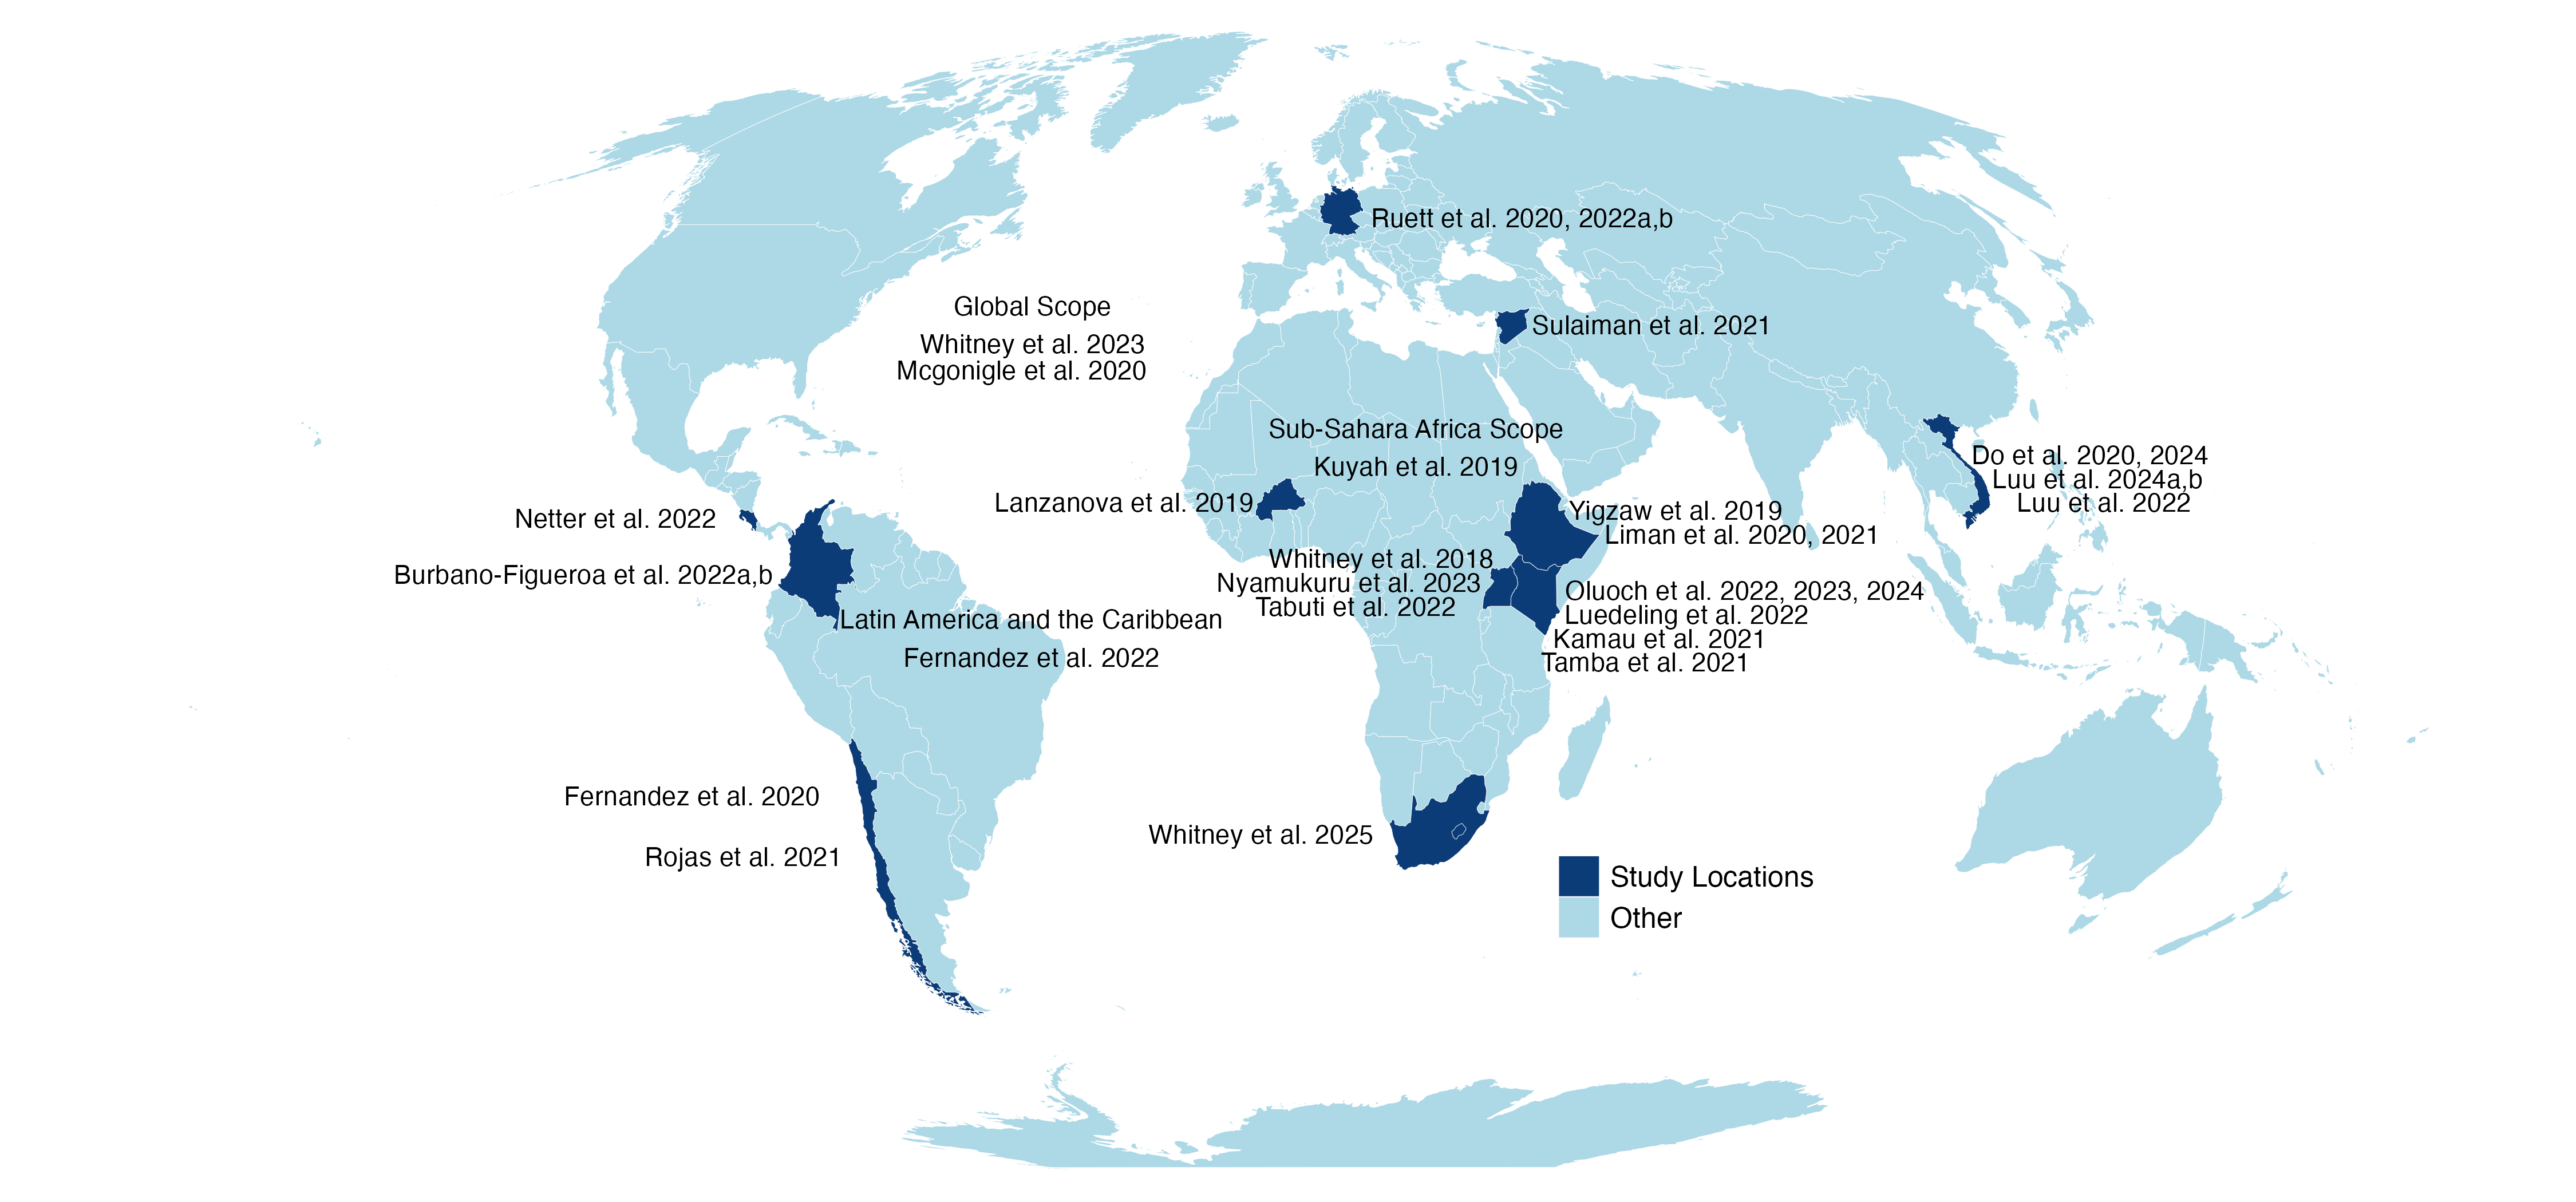
\includegraphics[width=10in,]{figures/plot_study_locations_map} 

}

\caption{\label{fig:plot_study_locations_map} Geographical distribution of the research contributions presented in this thesis}\label{fig:plot_study_locations_map}
\end{figure}

\end{landscape}

Several studies in this thesis evaluate agricultural certification
schemes and their implications for sustainability and economic
resilience. We prioritize interventions in banana plantations balancing
climate adaptation, farm productivity, and certification incentives in
Latin America and the Caribbean (Fernandez \emph{et al.} 2022)
\protect\hyperlink{fernandez_prioritizing_2022}{Paper 4} assesses carbon
certification for agroforestry projects in Costa Rica (Netter \emph{et
al.} 2022) \protect\hyperlink{netter_agroforestry_2022}{Paper 7} and
address the challenges of livestock emissions modeling in smallholder
farms in Kenya (Luedeling \emph{et al.} 2022)
\protect\hyperlink{luedeling_limitations_2022}{Paper 15}.

Beyond certification systems, the work presented also covers
horticultural production systems, with studies on economic risk in pest
management for diversified farms (Burbano-Figueroa \emph{et al.} 2022a)
\protect\hyperlink{burbano-figueroa_farm-planning_2022}{Paper 22}. We
assess disease management in ornamental plant production (Ruett \emph{et
al.} 2022a) \protect\hyperlink{ruett_assessing_2022}{Paper 24} and
(Ruett \emph{et al.} 2020)
\protect\hyperlink{ruett_model-based_2020}{Paper 25}. We assess ways to
enhance the climate resilience of deciduous fruit production in Chile
(Rojas \emph{et al.} 2021) \protect\hyperlink{rojas_adapting_2021}{Paper
16} and address the prospects of decreasing winter chill for these
production systems (Fernandez \emph{et al.} 2020)
\protect\hyperlink{fernandez_prospects_2020}{Paper 29}.

The work also covers socio-ecological resilience and traditional
ecological knowledge. We assess the cultural, ecological, and
nutritional value of wild edible plants in Kenya for conservation
strategies that align with Indigenous resource management (Oluoch
\emph{et al.} 2022) \protect\hyperlink{oluoch_integrated_2022}{Paper 12}
and (Oluoch \emph{et al.} 2024)
\protect\hyperlink{oluoch_predicted_2024}{Paper 18}. We study the
cultural dimensions of agroecology and resource use of Yerba Maté in
Syria (Sulaiman \emph{et al.} 2021)
\protect\hyperlink{sulaiman_socio-cultural_2021}{Paper 27}.

The work outlines the development of transdisciplinary decision-making
frameworks that facilitate collaboration between researchers,
policymakers, and practitioners. The approaches support science-policy
integration and multi-stakeholder decision-making (McGonigle \emph{et
al.} 2020) \protect\hyperlink{mcgonigle_knowledge_2020}{Paper 17}. We
applied a holistic sustainability assessment to evaluate the long-term
viability of organic and conventional farming in Kenyan smallholder
farming systems (Kamau \emph{et al.} 2021)
\protect\hyperlink{kamau_holistic_2021}{Paper 32}. The work includes
climate services and stakeholder-inclusive approaches Luu \emph{et al.}
(2024a), Luu \emph{et al.} (2022), Luu \emph{et al.} (2024b) Papers 6,
13, 14, that address the scaling of agro-climate services, emphasizing
collaborative planning for sustainable outcomes.

Several papers delve into biodiversity conservation and ecological
sustainability. Studies such as Do \emph{et al.} (2020), Kuyah \emph{et
al.} (2019), Oluoch \emph{et al.} (2022), Oluoch \emph{et al.} (2024),
Oluoch \emph{et al.} (2023), Nyamukuru \emph{et al.} (2023), Tabuti
\emph{et al.} (2022) Papers 5, 8, 12, 18, 26, 30, 31, explore themes
like wild edible plants, habitat restoration, and species prioritization
in Sub-Saharan Africa, showcasing the integration of local knowledge
with empirical modeling (Fig. \ref{fig:plot_thematic_areas}).

\begin{landscape}


\begin{figure}[H]

{\centering 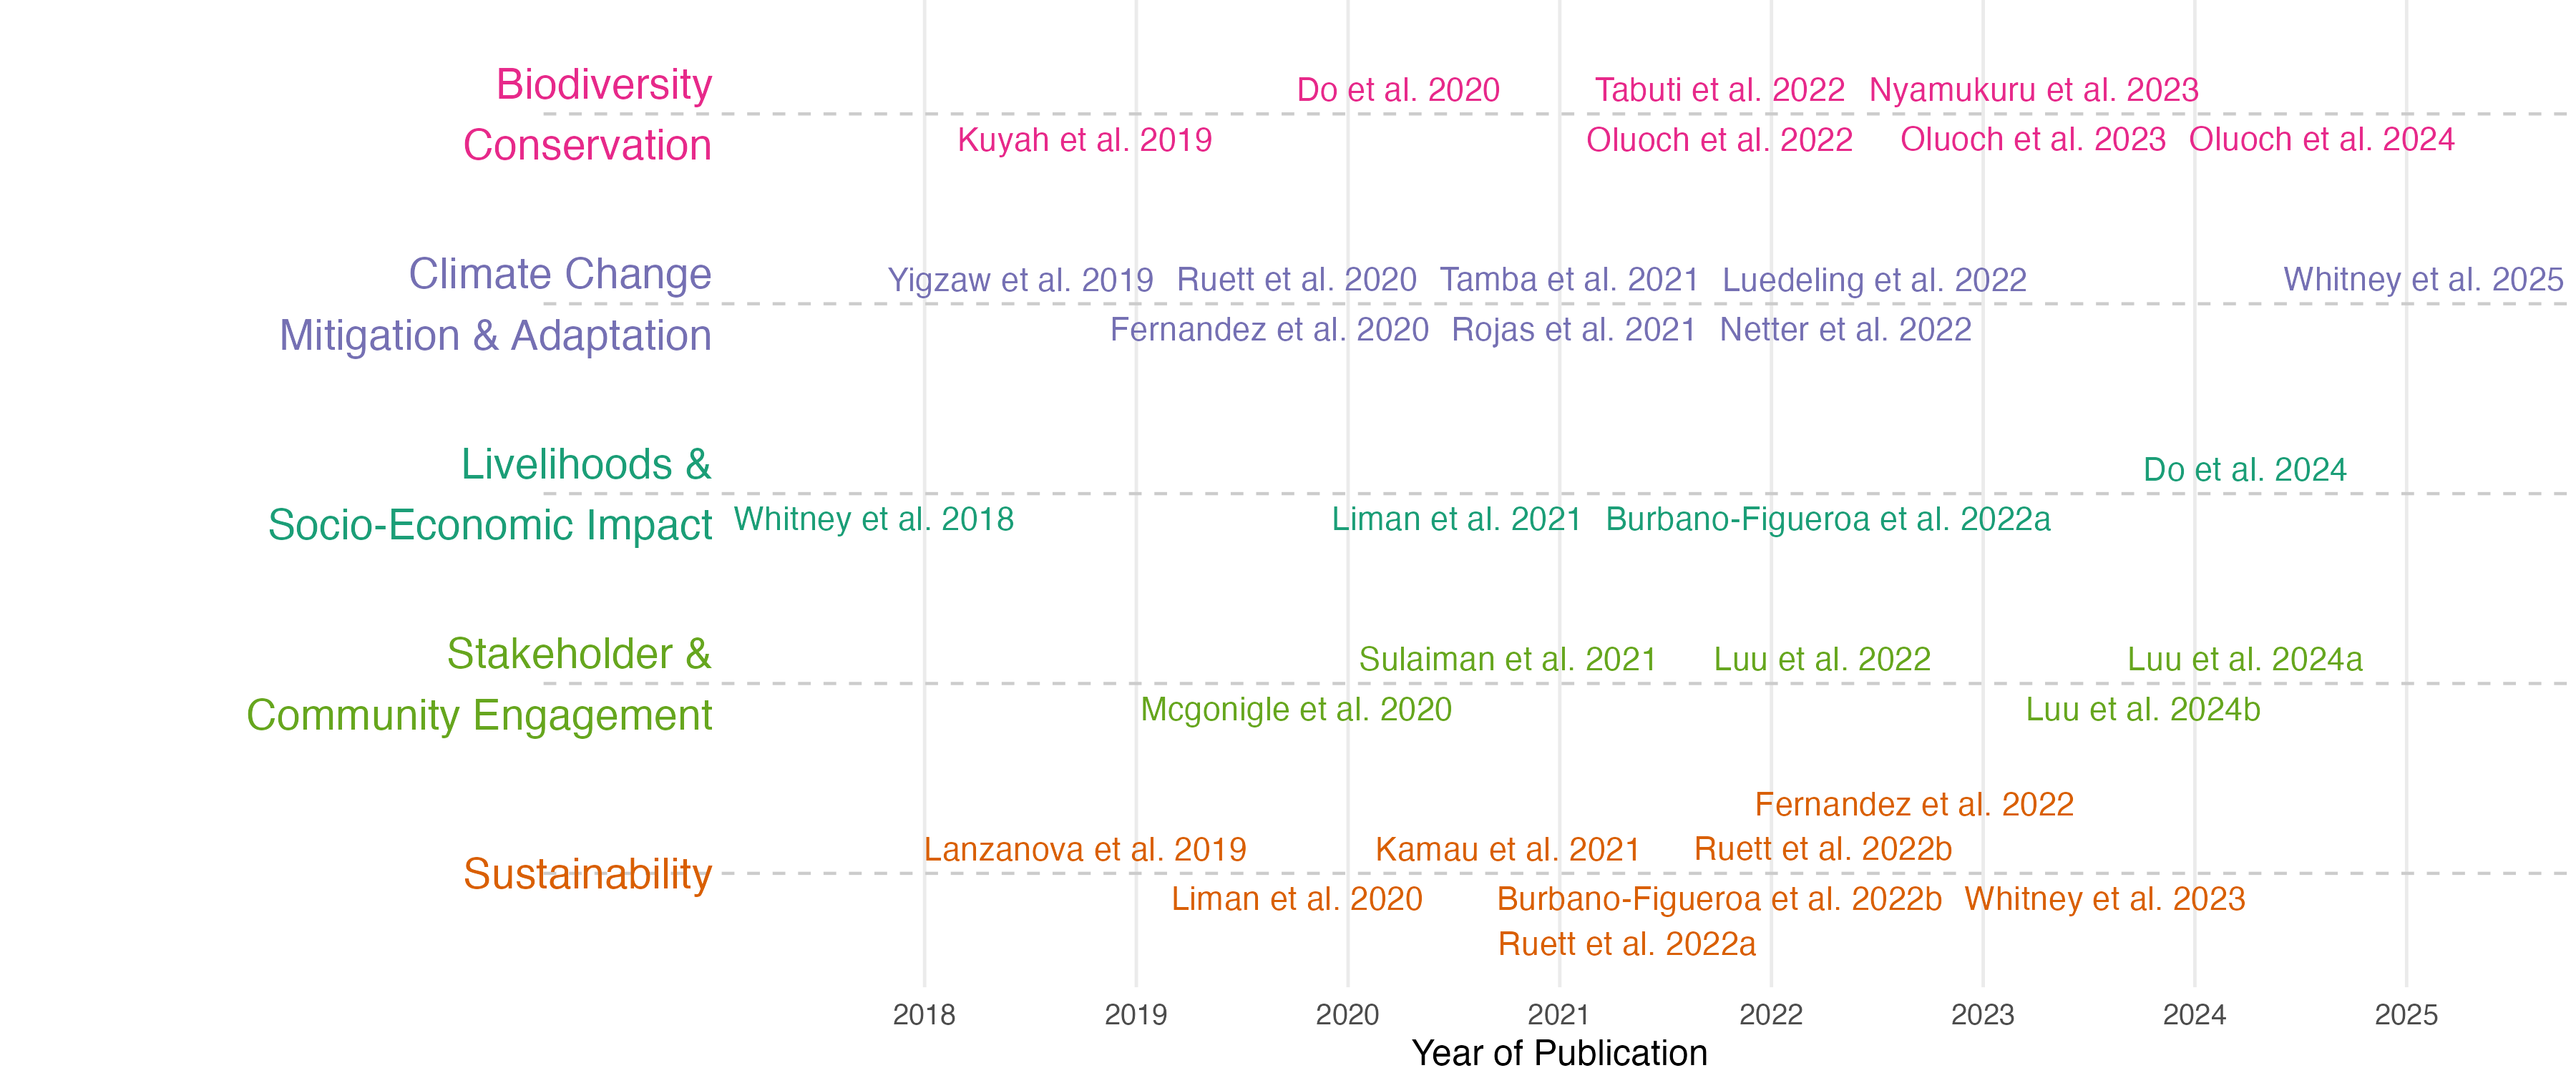
\includegraphics[width=1\linewidth,]{figures/plot_thematic_areas} 

}

\caption{\label{fig:plot_thematic_areas}Thematic areas of the research contributions presented in this thesis}\label{fig:plot_thematic_areas}
\end{figure}

\end{landscape}

\newpage

\hypertarget{authors-role-in-each-paper}{%
\section*{Author's role in each
paper}\label{authors-role-in-each-paper}}
\addcontentsline{toc}{section}{Author's role in each paper}

Throughout my research, I have played diverse roles in various projects,
from leading conceptualization and execution to helping supervise
students and securing funding. My first-author papers reflect my central
involvement in writing, formal analysis, and project leadership. Open
Access publication for papers during my time at the University of Bonn
was made possible through funding organized by Projekt DEAL.

I led Whitney \emph{et al.} (2018b) as part of the Competitive Research
Grants for Innovative Methods and Metrics for Agriculture and Nutrition
Actions (IMMANA), with funding secured by Prof.~Dr.~Eike Luedeling. I
contributed to refining the proposal, planning, and executing the
project. Whitney \emph{et al.} (2018d) marked my first post-PhD
publication, supported by the World Agroforestry Centre (ICRAF) as a
working paper, with parts later incorporated into Whitney \emph{et al.}
(2018b). In Whitney \emph{et al.} (2023), I contributed as an adviser
within the INTERFACES and LANUSYNCON projects, funded by the German
Federal Ministry of Education and Research (BMBF). I also helped
Prof.~Dr.~Lisa Biber-Freudenberger secure funding for these initiatives.
Whitney \emph{et al.} (2025) was a product of my leadership as the lead
author, with support from CGIAR's Water, Land, and Ecosystems (WLE)
program (Grant No.~D-0341) and environmental flow hydrology data
provided by USAID.

As the last author on several papers, I primarily guided the conceptual
direction, helped supervise research, and ensured strong research
outputs. Do \emph{et al.} (2020) stemmed from my work with an MSc
student, where I provided significant input on R programming, research
design, and conceptualization, alongside securing DAAD funding for
fieldwork in Vietnam. Similarly, I conceptualized Tabuti \emph{et al.}
(2022), supported through the ENRECA project at Gulu University,
assisting Prof.~Dr.~John Tabuti in securing funding and linking the work
to my R package Whitney (2021). In Luu \emph{et al.} (2024a), I was
deeply involved in modeling and writing and helped the lead author
secure funding through the Schlumberger Foundation's Faculty for the
Future Program. For Netter \emph{et al.} (2022), I helped supervise the
MSc student, performed formal analysis in R, formulated the models, and
facilitated ASA program scholarship funding via the German Federal
Ministry for Economic Cooperation and Development (BMZ).

In my role as a middle author, I frequently contributed to
conceptualization, programming, model development, and writing. In Kuyah
\emph{et al.} (2019), I worked closely with the first author on
assessment, statistics, and writing, assisting in securing funding from
the Alexander von Humboldt Foundation. My collaboration with AFLI and
CIFOR-ICRAF Vietnam led to Do \emph{et al.} (2024), where I helped
supervise the PhD student I had previously worked with during their MSc.
The project was part of Can Agroforestry Contribute to Sustainable
Development in Sloping Upland Areas of the Mekong Region? and received
funding from the Academy for International Agricultural Research
(ACINAR).

I was a key contributor to McGonigle \emph{et al.} (2020), collaborating
with CGIAR colleagues to secure WLE funding for sustainability research.
In Kamau \emph{et al.} (2021), I helped supervise the PhD student,
contributing to conceptualization and writing. My work in Lanzanova
\emph{et al.} (2019) extended to conceptualizing the project, leading
fieldwork, and developing models, supported by CGIAR's TAI research
initiative in the Northern Volta River Basin. In Yigzaw \emph{et al.}
(2019), I helped supervise the PhD student and led model development in
R, with funding from DAAD under the ``A World Without Hunger''
initiative.

My contributions to Oluoch \emph{et al.} (2022), Oluoch \emph{et al.}
(2023), and Oluoch \emph{et al.} (2024) included working with the PhD
student, leading data analysis, and programming models in R. I also
supported Prof.~Dr.~Christine Schmitt in securing BMZ-GIZ funding
through FIA and assisted the student in obtaining a `Get Finished'
scholarship from the University of Bonn. Similarly, in Fernandez
\emph{et al.} (2022), I led the project, worked closely on model
development, and helped secure funding from GIZ's ABNB initiative.

My role in Fernandez \emph{et al.} (2020) and Rojas \emph{et al.} (2021)
involved helping supervise the graduate students who were the lead
authors, guiding conceptualization, model development, and R
programming, as well as assisting Prof.~Dr.~Luedeling in securing PASIT
funding from BMBF. In Luu \emph{et al.} (2022) and Luu \emph{et al.}
(2024b), I helped supervise the PhD student and contributed to model
development, securing funding from the Schlumberger Foundation.

For Ruett \emph{et al.} (2022a), Ruett \emph{et al.} (2022b), and Ruett
\emph{et al.} (2020), I helped supervise the PhD student, contributed to
conceptualization, and played a central role in model development and R
programming. I also assisted Prof.~Dr.~Eike Luedeling in obtaining
funding from Stiftung Zukunft NRW for the INRUGA project. Similarly, in
Tamba \emph{et al.} (2021), I helped supervise the student and played a
major role in model development and R programming.

In Luedeling \emph{et al.} (2022), I contributed to the
conceptualization and development of the manuscript in collaboration
with the co-authors. My role included refining the methodological
approach, reviewing key arguments, and ensuring the clarity of the final
publication.

For Burbano-Figueroa \emph{et al.} (2022b) and Burbano-Figueroa \emph{et
al.} (2022a), I was responsible for methodological contributions,
particularly in structuring the analytical approach alongside the lead
authors. Additionally, I played a role in data visualization and
substantially revised the manuscripts, ensuring coherence in framing and
interpretation.

My work extended to Liman Harou \emph{et al.} (2020) and Liman Harou
\emph{et al.} (2021), where I helped supervise the PhD student and
contributed extensively to conceptualization, writing, and programming.
For Sulaiman \emph{et al.} (2021), I helped supervise the PhD student,
contributed to conceptualization, and led model development in R, basing
the analysis on my Whitney (2021) package. I also led data analysis and
model programming for Nyamukuru \emph{et al.} (2023), assisting the lead
author in securing funding through the NORHED program (UGA-13/0019)
under NORAD.

\newpage

\hypertarget{rationale}{%
\section*{Rationale}\label{rationale}}
\addcontentsline{toc}{section}{Rationale}

Sustainable development interventions must navigate difficult trade-offs
between improving human welfare---particularly for smallholder farming
communities---and protecting fragile ecological systems. Development
decisions in high-biodiversity areas are challenged by the complexity of
socio-ecological systems, limited reliable data, and deep uncertainty
surrounding future outcomes. Agricultural systems operate within a
landscape of accelerating climate change, resource constraints, and
socio-economic pressures.

My research addresses these challenges by integrating decision analysis
and agroecology to improve decision-making under uncertainty. Over the
past six years, I have developed probabilistic decision-support models
that structure uncertainty in agricultural and conservation planning
(e.g., Whitney \emph{et al.} 2018b). By applying expert-elicited
probabilistic models and Monte Carlo simulations, I have provided
structured approaches for evaluating intervention efficacy in
agroecology, land-use planning, and biodiversity conservation.

As climate change, biodiversity loss, and resource scarcity present
increasing risks to smallholder farmers, my work has demonstrated how
decision-support tools can enhance agricultural planning. I have applied
probabilistic modeling to agroforestry decision-making (Do \emph{et al.}
2024) and water resource management (Lanzanova \emph{et al.} 2019),
showing how structured uncertainty analysis supports sustainable
land-use strategies. My studies on Bayesian networks (Whitney \emph{et
al.} 2023) have also provided insights into improving decision-making in
agroecology by integrating expert knowledge and participatory
approaches.

At the core of my research is the use of probabilistic modeling to
quantify risks, trade-offs, and system dynamics in data-limited
environments. Unlike conventional deterministic models, my frameworks
explicitly incorporate probability distributions, expert knowledge, and
participatory inputs, making them more adaptive to real-world
conditions. By applying these methods, I have improved the transparency
and robustness of agricultural and environmental planning.

Beyond agricultural decision-making, my research has extended to water
resource management, pest control, carbon markets, and climate
adaptation. Studies such as Fernandez \emph{et al.} (2022) on climate
adaptation strategies and Do \emph{et al.} (2020) on agroforestry
adoption risks have demonstrated how structured decision-support
frameworks improve intervention design. These contributions underscore
the importance of integrating expert knowledge, participatory modeling,
and uncertainty-enabled decision analysis in sustainability science.

My work is rooted in transdisciplinary collaboration. By integrating
expert knowledge, local perspectives, and structured decision analysis,
I have developed decision-support tools that are contextually relevant
and actionable. The combination of probabilistic reasoning,
participatory modeling, and applied agroecology has advanced decision
science for sustainable agriculture, ensuring that scientific insights
translate into tangible, real-world impact.

The specific aims of my research include:

\begin{itemize}
\item
  \textbf{Designing and implementing decision-support models} to assess
  sustainable development strategies for smallholder farming
  communities. These models identify interventions that maximize
  socio-economic and ecological benefits by evaluating their impact on
  biodiversity and human livelihoods, ensuring sustainability at both
  community and environmental levels.
\item
  \textbf{Co-developing the modeling approach with local experts,
  Indigenous communities, and decision-makers.} By adopting a
  participatory approach, these models incorporate traditional
  conservation practices and Indigenous knowledge, adapting global
  strategies to specific local contexts (Fig.
  \ref{fig:Figures/Model_Dev_Flow}).
\item
  \textbf{Exploring synergies and trade-offs between economic
  development, gender equality, and environmental sustainability},
  particularly in alignment with the Sustainable Development Goals
  (SDGs).
\end{itemize}

\begin{figure}[H]

{\centering \includegraphics[width=1\linewidth,]{figures/Model_Dev_Flow} 

}

\caption{\label{fig:Figures/Model_Dev_Flow}Overview of the model development process for generating model forecasts. Adapted from the author’s research.}\label{fig:Figures/Model_Dev_Flow}
\end{figure}

My research draws on insights from human ecology, decision theory, and
agroecology to develop practical solutions (Fig.
\ref{fig:Figures/ERC_Venn}). Studies such as Altieri (2002) highlight
the importance of incorporating local farming knowledge into sustainable
agriculture. My work contributes to this literature by integrating
expert-elicited models and decision analysis into agroecological
research, ensuring that decision-making tools remain contextually
relevant and practically applicable.

\begin{figure}[H]

{\centering \includegraphics[width=1\linewidth,]{figures/ERC_Venn} 

}

\caption{\label{fig:Figures/ERC_Venn}Venn diagram illustrating the theoretical overlap in research approaches. Adapted from the author’s research.}\label{fig:Figures/ERC_Venn}
\end{figure}

This research integrates three key areas:

\begin{enumerate}
\def\labelenumi{\arabic{enumi}.}
\item
  \textbf{Decision Analysis} -- Providing structured methodologies for
  evaluating risks and outcomes in development decisions.
\item
  \textbf{Agroecology} -- Focusing on sustainable agricultural practices
  and ecological resilience.
\item
  \textbf{Human Ecology} -- Emphasizing local knowledge and
  socio-cultural contexts in decision-making.
\end{enumerate}

This transdisciplinary framework supports sustainable development by
balancing human well-being with ecological sustainability through
tailored decision-support models. My studies on participatory modeling,
such as Whitney \emph{et al.} (2023), have demonstrated how
expert-elicited knowledge and stakeholder engagement enhance
decision-making under uncertainty.

As Howard \& Abbas (2015) outlined, decision analysis provides
structured methodologies for evaluating alternatives and potential
outcomes under uncertainty. My work applies these principles in
agroecology and conservation planning, integrating data, expert
judgment, and stakeholder input to optimize sustainability strategies.
While causal models such as those described by Pearl \& Mackenzie (2018)
are widely used in structured decision-making, my work has shown that
conventional models often fail to capture the high uncertainty and
complexity inherent in smallholder farming systems. My research adapts
these tools to community-driven, localized development strategies,
demonstrating how decision science can be effectively applied to
agroecology and conservation.

Drawing from human ecology, I have employed \textbf{progressive
contextualization} (Vayda 1983), tracing causal chains from specific
land-use decisions to broader socio-economic and environmental factors.
This iterative, problem-driven approach has been particularly useful in
agroecological research, ensuring that interventions are grounded in
real-world dynamics rather than static models. By embedding research
within local communities, my work has avoided rigid system boundaries,
allowing for emergent complexities to shape decision models dynamically.

\textbf{Key Contributions:}

\begin{itemize}
\item
  \textbf{Structured decision-support models}: Applying Monte Carlo
  simulations, Bayesian networks, and expert-elicited probability
  distributions to assess intervention impacts.
\item
  \textbf{Participatory modeling}: Engaging local stakeholders to ensure
  decision models reflect real-world constraints and opportunities.
\item
  \textbf{Transdisciplinary integration}: Bridging decision analysis,
  agroecology, and human ecology to improve agricultural sustainability
  planning.
\end{itemize}

By refining probabilistic decision models and participatory frameworks,
my research has provided actionable decision-support tools that enhance
sustainability outcomes. These findings contribute to ongoing debates in
decision science, agroecology, and conservation planning, demonstrating
the practical application of uncertainty-enabled decision analysis in
real-world sustainability challenges.

\newpage

\hypertarget{theoretical-foundations}{%
\section*{Theoretical Foundations}\label{theoretical-foundations}}
\addcontentsline{toc}{section}{Theoretical Foundations}

The theoretical foundations of this habilitation integrate systems
thinking, decision science, and participatory research to address
complexity in agroecology. Rather than an exhaustive review, this
synthesis highlights key contributions that shaped my approach. The
discussion is structured by thematic relevance rather than chronology.

Grounded in systems thinking, human ecology, and transdisciplinary
research, my approach integrates probabilistic modeling, participatory
decision-making, and knowledge co-production. Theoretical insights from
Meadows, Ostrom, Vayda, Howard, Keeney, Claxton, Lang, Chambers, and
Norström inform the development of decision-support frameworks that
account for uncertainty, stakeholder engagement, and sustainability in
agroecological systems. Agroecology theory, particularly the
contributions of Altieri and Gliessman, provide the ethical and
conceptual foundation for my research.

\hypertarget{donella-meadows-and-systems-thinking}{%
\subsection*{Donella Meadows and Systems
Thinking}\label{donella-meadows-and-systems-thinking}}
\addcontentsline{toc}{subsection}{Donella Meadows and Systems Thinking}

Donella Meadows' work in systems thinking and leverage points provides a
theoretical foundation for understanding and managing complex
agroecosystems. She demonstrated that systems are nonlinear and
counterintuitive, meaning that interventions often fail or produce
unintended consequences when they do not align with the underlying
system structure (Meadows 1999). Meadows' leverage points framework
categorizes interventions from minor parameter adjustments to deep
structural and paradigm shifts, underscoring the importance of
system-wide transformation over incremental changes.

Her system dynamics modeling highlights feedback loops, delays, and
emergent behaviors, illustrating the interplay of agricultural policies,
resource use, and ecosystem dynamics. By framing decision-making within
complex, adaptive systems, Meadows' insights help structure holistic
agroecological interventions, ensuring that solutions address root
causes rather than symptoms and support long-term sustainability.

\hypertarget{technocratic-vs.-participatory-approaches-insights-from-elinor-ostrom}{%
\subsection*{Technocratic vs.~Participatory Approaches: Insights from
Elinor
Ostrom}\label{technocratic-vs.-participatory-approaches-insights-from-elinor-ostrom}}
\addcontentsline{toc}{subsection}{Technocratic vs.~Participatory
Approaches: Insights from Elinor Ostrom}

Agricultural interventions have historically followed top-down,
technocratic models, prioritizing yield maximization and economic
efficiency, while often neglecting social and ecological sustainability.
Elinor Ostrom challenged this centralized approach by demonstrating that
resource users can self-organize to manage common-pool resources without
requiring external control (Ostrom 2009). Ostrom's framework emphasizes
decentralized governance, monitoring, and collective decision-making for
sustainable resource management.

By outlining design principles for robust common-pool resource
management, Ostrom provided a theoretical foundation for participatory
decision-making, adaptive governance, and transdisciplinary
sustainability research. Her work reinforces the importance of inclusive
stakeholder engagement in agroecology, ensuring that farmers, Indigenous
communities, and local institutions play an active role in shaping
sustainable agricultural systems.

\hypertarget{progressive-contextualization-insights-from-andrew-vayda}{%
\subsection*{Progressive Contextualization: Insights from Andrew
Vayda}\label{progressive-contextualization-insights-from-andrew-vayda}}
\addcontentsline{toc}{subsection}{Progressive Contextualization:
Insights from Andrew Vayda}

Andrew Vayda's progressive contextualization method provides a flexible,
empirical approach to studying human-environment interactions without
imposing rigid theoretical frameworks (Vayda 1983). Instead of starting
with predefined models, his approach traces causal chains from specific
events, working backward to identify relevant contextual factors.

This problem-driven, iterative method allows research to adapt
dynamically to emerging findings, avoiding disciplinary biases that
often constrain agricultural and environmental studies. His work in
human ecology demonstrates that both transitory and persistent
ecological phenomena can be understood through focused, adaptable
investigations, making it particularly relevant to agroecology.

Vayda's approach has been widely applied in resource management,
environmental change, and sustainability research, where complex,
shifting variables require iterative analysis. By prioritizing empirical
flexibility over static models, progressive contextualization offers a
practical framework for transdisciplinary research, enhancing
agroecological resilience, participatory decision-making, and adaptive
governance.

\hypertarget{decision-analysis-insights-from-ron-howard-and-ali-abbas}{%
\subsection*{Decision Analysis: Insights from Ron Howard and Ali
Abbas}\label{decision-analysis-insights-from-ron-howard-and-ali-abbas}}
\addcontentsline{toc}{subsection}{Decision Analysis: Insights from Ron
Howard and Ali Abbas}

Howard and Abbas formalize decision analysis as a structured approach to
managing uncertainty, integrating probability theory, utility functions,
and Bayesian reasoning (Howard \& Abbas 2015). They emphasize that
decision-making is an iterative process, where beliefs and preferences
are continuously refined based on new information. They emphasize Value
of Information (VOI) and sensitivity analysis as tools to improve
decision quality and optimize research resource allocation in uncertain
environments.

This framework is particularly relevant to agroecology, policy design,
and resource management, where uncertainty in ecological and
socio-economic systems demands structured, probabilistic approaches. By
applying Howard and Abbas' principles, agroecological decision-making
can become more transparent, data-informed, and adaptive, enhancing the
effectiveness of interventions and long-term sustainability strategies.

\hypertarget{multi-objective-decision-analysis-insights-from-ralph-keeney}{%
\subsubsection*{Multi-Objective Decision Analysis: Insights from Ralph
Keeney}\label{multi-objective-decision-analysis-insights-from-ralph-keeney}}
\addcontentsline{toc}{subsubsection}{Multi-Objective Decision Analysis:
Insights from Ralph Keeney}

Ralph Keeney's work focuses on decisions with multiple objectives, his
work focuses on preferences and value trade-Offs and extends decision
analysis beyond single-objective optimization, formalizing
multi-objective decision-making to address trade-offs between competing
economic, environmental, and social factors (Keeney \& Raiffa 1993). His
framework, known as value-focused thinking, requires decision-makers to
explicitly define and structure their preferences before evaluating
alternatives, ensuring that decisions align with broader goals rather
than reactive constraints. Keeney applies multi-attribute utility theory
and preference elicitation to quantify trade-offs and integrate
stakeholder values.

In agroecology, where interventions must balance productivity,
conservation, and socio-economic priorities, Keeney's methods offer a
structured, transparent framework for evaluating complex choices. His
work strengthens participatory decision-making, ensuring that
stakeholder preferences and long-term sustainability goals guide
agricultural and environmental policies.

\hypertarget{value-of-information-in-decision-analysis-insights-from-karl-claxton}{%
\subsubsection*{Value of Information in Decision Analysis: Insights from
Karl
Claxton}\label{value-of-information-in-decision-analysis-insights-from-karl-claxton}}
\addcontentsline{toc}{subsubsection}{Value of Information in Decision
Analysis: Insights from Karl Claxton}

Karl Claxton's research formalizes decision-making under uncertainty,
particularly through Value of Information (VOI) analysis, which
quantifies the benefit of reducing uncertainty before committing to an
action (Claxton \emph{et al.} 2012). His work ensures that resources are
allocated efficiently, demonstrating how Bayesian decision analysis can
evaluate the expected value of perfect and imperfect information (EVPI
\& EVSI) to guide investment in data collection, research, and policy
interventions.

Claxton's contributions are widely applied in health economics and
policy, where VOI helps prioritize research funding and assess
intervention cost-effectiveness. More broadly, his methods are relevant
to resource management, risk assessment, and sustainability, where
structured uncertainty analysis improves decision quality and enhances
strategic planning for complex, data-limited systems (Claxton \emph{et
al.} 2012)

\hypertarget{emerging-transdisciplinary-approaches-in-development-research}{%
\subsection*{Emerging Transdisciplinary Approaches in Development
Research}\label{emerging-transdisciplinary-approaches-in-development-research}}
\addcontentsline{toc}{subsection}{Emerging Transdisciplinary Approaches
in Development Research}

\hypertarget{transdisciplinary-research-in-sustainability-science-insights-from-daniel-lang}{%
\subsubsection*{Transdisciplinary Research in Sustainability Science:
Insights from Daniel
Lang}\label{transdisciplinary-research-in-sustainability-science-insights-from-daniel-lang}}
\addcontentsline{toc}{subsubsection}{Transdisciplinary Research in
Sustainability Science: Insights from Daniel Lang}

Lang's work highlights the need for new knowledge production methods in
sustainability science, emphasizing transdisciplinary, participatory,
and community-based research as essential for addressing complex
societal challenges (Lang \emph{et al.} 2012). He argues that
integrating diverse knowledge systems - scientific and local - enhances
decision-making, aligns research with societal needs, and fosters
stakeholder ownership of solutions.

His conceptual model for transdisciplinary sustainability research
synthesizes principles from various empirical studies, structuring best
practices for co-producing knowledge in sustainability science. By
examining case studies across multiple continents, Lang identifies
challenges and coping strategies for effectively implementing
interactive and participatory research approaches.

His framework is particularly relevant for agroecology, policy design,
and resource management, where multi-stakeholder engagement and
knowledge co-production improve the relevance and impact of research.
Lang's work provides a structured approach for integrating science and
practice, strengthening sustainability transitions through inclusive and
adaptive decision-making.

\hypertarget{adaptive-pluralism-and-participatory-development-insights-from-robert-chambers}{%
\subsubsection*{Adaptive Pluralism and Participatory Development:
Insights from Robert
Chambers}\label{adaptive-pluralism-and-participatory-development-insights-from-robert-chambers}}
\addcontentsline{toc}{subsubsection}{Adaptive Pluralism and
Participatory Development: Insights from Robert Chambers}

Robert Chambers advocates for adaptive pluralism in development studies,
emphasizing bottom-up, participatory approaches to address poverty and
sustainability challenges (Chambers 2010). He critiques top-down,
technocratic paradigms, arguing that local knowledge, experiential
learning, and flexible methodologies are essential for effective
interventions.

Chambers highlights that poverty is multidimensional and
context-specific, requiring iterative, inclusive decision-making that
empowers marginalized communities. His work aligns with
transdisciplinary research and participatory decision analysis,
reinforcing the importance of stakeholder engagement, co-produced
knowledge, and decentralized governance in addressing complex
sustainability challenges.

By integrating participatory learning and action-oriented research,
Chambers' approach provides a practical foundation for agroecology,
rural development, and sustainability science, ensuring that solutions
are locally relevant, adaptable, and community-driven.

\hypertarget{knowledge-co-production-in-sustainability-science-insights-from-albert-norstruxf6m-et-al.}{%
\subsubsection*{Knowledge Co-Production in Sustainability Science:
Insights from Albert Norström et
al.~}\label{knowledge-co-production-in-sustainability-science-insights-from-albert-norstruxf6m-et-al.}}
\addcontentsline{toc}{subsubsection}{Knowledge Co-Production in
Sustainability Science: Insights from Albert Norström et al.~}

Norström et al.~define knowledge co-production as an approach that
integrates academic and non-academic actors to tackle complex
sustainability challenges more effectively than traditional scientific
methods (Norström \emph{et al.} 2020). Recognizing inconsistencies in
co-production definitions, they propose four core principles:
context-based collaboration, pluralism, goal-orientation, and iterative
learning.

Their framework provides practical guidance for structuring
co-production through shared problem definitions, power-balanced
collaboration, and adaptive learning cycles. Stakeholder-driven,
participatory methodologies enhance sustainability research by ensuring
relevance, legitimacy, and impact.

In my approach to transdisciplinary development research, a defining
characteristic is that the aims, goals, and activities are co-defined
with stakeholders themselves, rather than being predetermined. This
aligns closely with Altieri's ethics in agroecology---``nothing about us
without us''---ensuring that research is not extractive but
participatory and context-driven.

Both \emph{emic} (insider) and \emph{etic} (external) perspectives play
a role in my work. While local perspectives are essential for shaping
interventions, an external lens is critical for understanding broader
development aims, causal mechanisms, and long-term impacts of
interventions. This balance helps ensure that development efforts are
not only locally relevant but also theoretically grounded and scalable.

A key example of this approach is my current project Nutrition
Intervention Forecasting and Monitoring (NIFAM) project funded by the
Federal Ministry of Food and Agriculture (BMEL), where we deliberately
included ``blank spaces'' throughout the proposal, leaving room for
activities to emerge through engagement with stakeholders. Rather than
imposing predefined interventions, we work with local actors to first
analyze food environments in depth and then co-develop interventions,
understand intervention goals, and describe the underlying causal
pathways by which the intervention will achieve the intended goals. We
work together to co-develop models, making explicit the assumed
relationships.

Local actors and researchers collaboratively shape the design and
implementation of interventions, fostering shared ownership and
adaptability. Together we describe the mechanisms by which interventions
lead to intended outcomes. This step involves mapping underlying
relationships using tools like directed acyclic graphs---to understand
and evaluate the theoretical and empirical connections between
interventions and their impacts. By distinguishing these two processes,
we maintain clarity in our methodology, ensuring that the collaborative
development of interventions and the rigorous investigation of causal
pathways each receive their appropriate focus.

\hypertarget{agroecology-theory-miguel-altieri-and-steven-gliessman}{%
\subsection*{Agroecology Theory: Miguel Altieri and Steven
Gliessman}\label{agroecology-theory-miguel-altieri-and-steven-gliessman}}
\addcontentsline{toc}{subsection}{Agroecology Theory: Miguel Altieri and
Steven Gliessman}

Agroecology integrates ecological principles, traditional knowledge, and
socio-economic factors to enhance resilience and sustainability in food
systems. It moves beyond conventional input-driven models, emphasizing
systems thinking, biodiversity, and the dynamic interactions between
human and natural ecosystems (Altieri 2002; Gliessman 2014). Central to
agroecology is the integration of scientific principles---spanning
ecology, sociology, economics, and policy---with participatory
approaches that engage local stakeholders.

Agroecology has emerged as a holistic and transformative approach to
agricultural development, integrating ecological and social principles
into food production systems. It has garnered widespread recognition for
its potential to address critical global challenges, including food
security, environmental degradation, and climate change. Agroecology
emphasizes biodiversity, education, consumer engagement, and governance
as essential elements for fostering sustainable agricultural systems
(Barrios \emph{et al.} 2020). It advocates for the sustainable
management of agricultural landscapes through strategies like crop
diversification, agroforestry, and integrated pest management, which
collectively enhance ecosystem services and improve resource efficiency
(Altieri 2012). By moving beyond conventional farming practices,
agroecology incorporates a deep understanding of ecosystem dynamics and
prioritizes social equity (Gliessman 2014).

Ecologically, agroecology applies principles of ecosystem functioning to
agricultural landscapes. It recognizes that diversified farming
systems---such as polycultures, agroforestry, and crop-livestock
integration---enhance nutrient cycling, pest regulation, and ecosystem
stability (Altieri 2002; Altieri 2012). These systems mimic natural
ecosystems, reducing reliance on external inputs while increasing
resilience to climatic and economic shocks. Agroecology also prioritizes
multi-functional landscapes, ensuring that food production, biodiversity
conservation, and ecosystem services are balanced (Gliessman 2014).

At a social level, agroecology is rooted in local knowledge systems,
participatory governance, and food sovereignty. It challenges top-down,
industrial agricultural models by emphasizing farmer autonomy and
localized decision-making (Altieri 2002). Agroecology promotes
co-production of knowledge, where scientific insights and farmer
experience are integrated to develop context-specific solutions
(Gliessman 2014). This participatory approach is essential for scaling
sustainable practices while maintaining cultural and ecological
diversity.

From a systems perspective, agroecology is a transition-oriented
framework, guiding food systems toward greater sustainability through
five levels of transformation (Gliessman 2014). These range from
efficiency-based improvements within existing systems to structural
changes in policies, markets, and governance that redefine how food is
produced, distributed, and consumed. Agroecology operates within complex
adaptive systems, requiring decision-support frameworks that integrate
uncertainty, feedback loops, and long-term sustainability goals (Altieri
2002).

Central to agroecology is the commitment to ecological balance,
biodiversity conservation, and socio-economic well-being. By reducing
reliance on external inputs, agroecological practices empower
smallholder farmers and bolster economic resilience (Méndez \emph{et
al.} 2013). These practices yield tangible benefits, such as improved
soil health, enhanced water retention, and increased crop productivity,
particularly in regions vulnerable to climate variability (Wezel
\emph{et al.} 2020). Additionally, agroecology plays a significant role
in climate change mitigation and adaptation by sequestering carbon and
lowering greenhouse gas emissions (Place \emph{et al.} 2022).

Agroecology provides pathways for transitioning to sustainable food
systems by co-creating knowledge with local stakeholders and
implementing practices that support biodiversity, equity, and
participatory governance (Wezel \emph{et al.} 2020). Effective
agroecological transitions require a comprehensive understanding of
political and economic dimensions, including social factors, labor
dynamics, markets and resources, social organization, and governance
structures (McKay \emph{et al.} 2024).

Agroecology's integration of scientific and traditional knowledge
ensures that solutions are context-specific and culturally relevant,
promoting food sovereignty and social justice (Place \emph{et al.}
2022). This integration positions agroecology as a vital strategy for
achieving Sustainable Development Goals, including SDG 2 (Zero Hunger),
SDG 13 (Climate Action), and SDG 15 (Life on Land) (UN 2015). By
harmonizing agricultural productivity with the conservation of ecosystem
services, agroecology paves the way for sustainable development in
diverse contexts, from rural landscapes to urban food systems (Tittonell
2014).

Despite its promise, agroecology faces challenges in widespread adoption
due to complexity and limited decision-support tools. The successful
implementation of agroecology hinges on active engagement with diverse
stakeholders---including researchers, farmers, NGOs, and
policymakers---to co-design innovations, identify economic
opportunities, and develop supportive policies (Russell \emph{et al.}
2023). There is a pressing need for research that bridges science and
practice to accelerate agroecological adoption. This includes
identifying enabling factors, such as policy support, participatory
research, and socio-technical systems, that catalyze agroecological
transitions in low and middle income countries (Jones \emph{et al.}
2022).

Despite its strengths, agroecology faces challenges in adoption due to
complexity, uncertainty, and the need for context-specific solutions.
Despite its theoretical strengths, the adoption and scaling of
agroecological practices remain limited, partly due to insufficient
tools for navigating trade-offs, assessing competing options, and
addressing systemic uncertainties. My research contributes by applying
probabilistic modeling, Monte Carlo simulations, and expert-elicited
frameworks to assess risks, benefits and trade-offs in agroecological
transitions. These methods can enhance the salience, legitimacy, and
credibility of agroecology by providing decision-makers with
transparent, evidence-based tools to support context-specific
interventions. Ultimately, this approach helps bridge the gap between
agroecological theory and practice, enabling more effective, scalable,
and contextually relevant solutions for sustainable agricultural
development.

\hypertarget{other-influential-perspectives}{%
\subsection*{Other Influential
Perspectives}\label{other-influential-perspectives}}
\addcontentsline{toc}{subsection}{Other Influential Perspectives}

The theoretical foundations of my work are influenced by ideas and
contributions from several thinkers whose work has shaped my
perspective, either directly or indirectly. Hans Rosling's ability to
translate complex global development data into accessible narratives has
fostered a deeper understanding of global health and socioeconomic
trends. Daniel Kahneman's pioneering research on decision-making and
cognitive biases offers essential insights into human behavior under
uncertainty, informing much of my work on decision analysis. Sir Ken
Robinson's advocacy for creativity in education challenges traditional
academic structures and offers valuable lessons for participatory
research and knowledge co-creation---key tenets in agroecological
transitions. David Quammen's writing, blending scientific rigor with
narrative storytelling, highlights the complexities of biodiversity loss
and zoonotic diseases, reinforcing the importance of ecological balance.
Thinkers such as Ludwig Wittgenstein and Albert Camus have shaped my
understanding of meaning, ethics, and human agency within complex
systems. John Visvader's explorations of ecological philosophy and
interconnectedness provide profound insights into human-nature
relationships, complementing the theoretical foundations of human
ecology and decision-making.

While these thinkers are not central to the methodological core of my
work, their intellectual contributions have subtly shaped my approach to
complexity, uncertainty, and transdisciplinary research. Their ideas
inform my broader reflections on the role of human agency, creativity,
and systemic thinking within the context of sustainable development and
agroecology.

\hypertarget{a-structured-and-adaptive-framework}{%
\subsection*{A Structured and Adaptive
Framework}\label{a-structured-and-adaptive-framework}}
\addcontentsline{toc}{subsection}{A Structured and Adaptive Framework}

These theoretical foundations provide a structured yet adaptive
framework for addressing the complexities of agroecology and sustainable
development. Systems thinking, social-ecological frameworks, and
decision analysis enable a holistic understanding of agricultural
systems, while transdisciplinary research and knowledge co-production
ensure that interventions are grounded in stakeholder priorities and
contextual realities. These frameworks collectively shape the
methodological innovations presented in this habilitation, ensuring that
research not only analyzes complex systems but also supports actionable,
stakeholder-driven solutions for a sustainable future.

Agroecology is a scientific field dedicated to understanding the complex
interactions among ecological, social, economic, and political systems
within agricultural landscapes. At the same time, it offers a
transformative approach to sustainable development by integrating
rigorous scientific research with practical, context-specific strategies
that enhance biodiversity, equity, and resilience. Agroecology
represents a transformative approach to sustainable development,
integrating ecological principles with agricultural practices to enhance
sustainability, equity, and resilience. As global food systems face
mounting challenges from climate change, resource scarcity, and
socio-economic inequities, agroecology provides a pathway to reconcile
the dual imperatives of ecological integrity and human well-being. By
fostering biodiversity, reducing reliance on external inputs, and
prioritizing local knowledge and participatory governance, agroecology
transcends traditional agricultural paradigms, addressing both global
sustainability goals and localized needs.

Central to the advancement of agroecology is the ability to navigate the
inherent complexity and uncertainty of agricultural systems. These
systems operate at the intersection of environmental, social, and
economic dimensions, making them highly dynamic and context-dependent.
Decision analytical methods, particularly probabilistic modeling and
decision-support frameworks, play a crucial role in this context. By
incorporating uncertainty into the evaluation of interventions, these
methods enable a more realistic and comprehensive assessment of
potential outcomes. They provide a structured approach for identifying
trade-offs, prioritizing actions, and designing strategies that align
with agroecological principles.

The advancement of agroecology as a transformative approach to
sustainable development requires integrated, transdisciplinary research
that embraces complexity, engages diverse stakeholders, and addresses
uncertainty. Throughout my work, I have sought to bridge the gap between
theoretical decision analysis and practical applications, emphasizing
tools and methods that empower decision-makers while aligning with the
needs and priorities of local communities.

Agroecology thrives at the intersection of ecology, sociology,
economics, and policy. My research underscores the importance of
transdisciplinary approaches in navigating the complex interdependencies
of agricultural systems. By collaborating with farmers, policymakers,
and researchers across disciplines, I have contributed to co-creating
solutions that are contextually relevant and scientifically robust.
Future research must continue to refine and expand decision-support
tools that accommodate increasing system complexity and uncertainty.
This includes developing scalable models that integrate diverse data
sources, leveraging advances in technology to enhance precision and
accessibility, and fostering deeper engagement with marginalized
communities to ensure inclusivity and equity in sustainable development.

My contributions span the development and application of probabilistic
decision tools, stochastic models, and participatory frameworks. These
methods have been instrumental in addressing critical challenges in
agriculture, including the adoption of agroforestry practices, the
management of climate risks, and the optimization of resource use in
diverse agricultural systems. By integrating empirical data with
Indigenous knowledge and stakeholder engagement, my work has
demonstrated the potential of agroecology to achieve interconnected
gains in food security, biodiversity conservation, and equitable
development.

\renewcommand{\thesection}{\arabic{section}}
\renewcommand{\thesubsection}{\thesection.\arabic{subsection}}

\newpage
\pagenumbering{arabic}

\hypertarget{introduction}{%
\section{Introduction}\label{introduction}}

This habilitation advances decision analysis in agroecology by
developing probabilistic models, identifying systemic leverage points,
and integrating participatory methods to improve decision-making under
uncertainty. It demonstrates applications across agroforestry,
hydrology, certification schemes, biodiversity conservation, and climate
services. By bridging probabilistic modeling, decision science, and
transdisciplinary research, the work supports sustainability
transformations. It clarifies complex decision environments and applies
structured decision-support tools to optimize land use, balance
productivity with conservation, and integrate diverse knowledge systems.

The habilitation is structured into two sections: the first advances
decision analytical methods in agroecology, while the second contributes
to methodological innovations in transdisciplinary research. These
sections draw on published studies employing structured decision models,
probabilistic analysis, and participatory methods to address key
challenges in sustainable agriculture.

The first section, \protect\hyperlink{chapter_one}{``Advancing
Agroecology through Decision Analytical Methods,''} explores how
decision analysis supports agroecological interventions by addressing
complexity, uncertainty, and trade-offs. Studies apply structured
decision models across domains such as agroforestry, horticulture, water
management, and climate adaptation. By incorporating probabilistic
reasoning and expert-elicited knowledge, these models offer robust
frameworks for evaluating interventions. In agroforestry, decision
models navigate ecological and socio-economic trade-offs, guiding
land-use decisions that balance productivity and sustainability. In
horticulture, they assess management strategies under resource
constraints and market fluctuations. Water management applications
integrate climate projections, hydrological data, and stakeholder input
to optimize resource allocation. As climate change reshapes agricultural
landscapes, decision analysis provides critical tools for adaptation,
mitigation, and cost-effective intervention.

The second section, \protect\hyperlink{chapter_two}{``Advancing Methods
in Transdisciplinarity and Agroecology,''} highlights methodological
innovations that connect agroecology with transdisciplinary research. It
emphasizes participatory approaches, stakeholder engagement, and
holistic evaluation frameworks that support knowledge co-creation and
agroecological innovation. These methods integrate scientific research
with local knowledge, foster cross-disciplinary collaboration, and
tailor interventions to community needs. The legitimacy and
effectiveness of agroecological practices is enhanced by involving
stakeholders in decision-making, ensuring research aligns with practical
realities. Holistic evaluation frameworks extend beyond cost-benefit
analyses, incorporating environmental, social, and economic dimensions
for a comprehensive sustainability assessment. Bridging science, policy,
and practice remains critical for translating research into meaningful
policy outcomes and tangible community benefits.

Together, these sections provide a foundation for advancing decision
analytical methods in agroecology while contributing to broader
methodological debates in transdisciplinary research. Through structured
models, probabilistic reasoning, and participatory approaches, this work
demonstrates how scientific rigor and practical application can address
complex sustainability challenges. Figure
\ref{fig:scatter_plot_applications_methods} illustrates the connection
between theoretical and applied dimensions, highlighting the role of
decision analysis in agroecological transitions across scales and
contexts.

\begin{landscape}

\begin{figure}[H]

{\centering 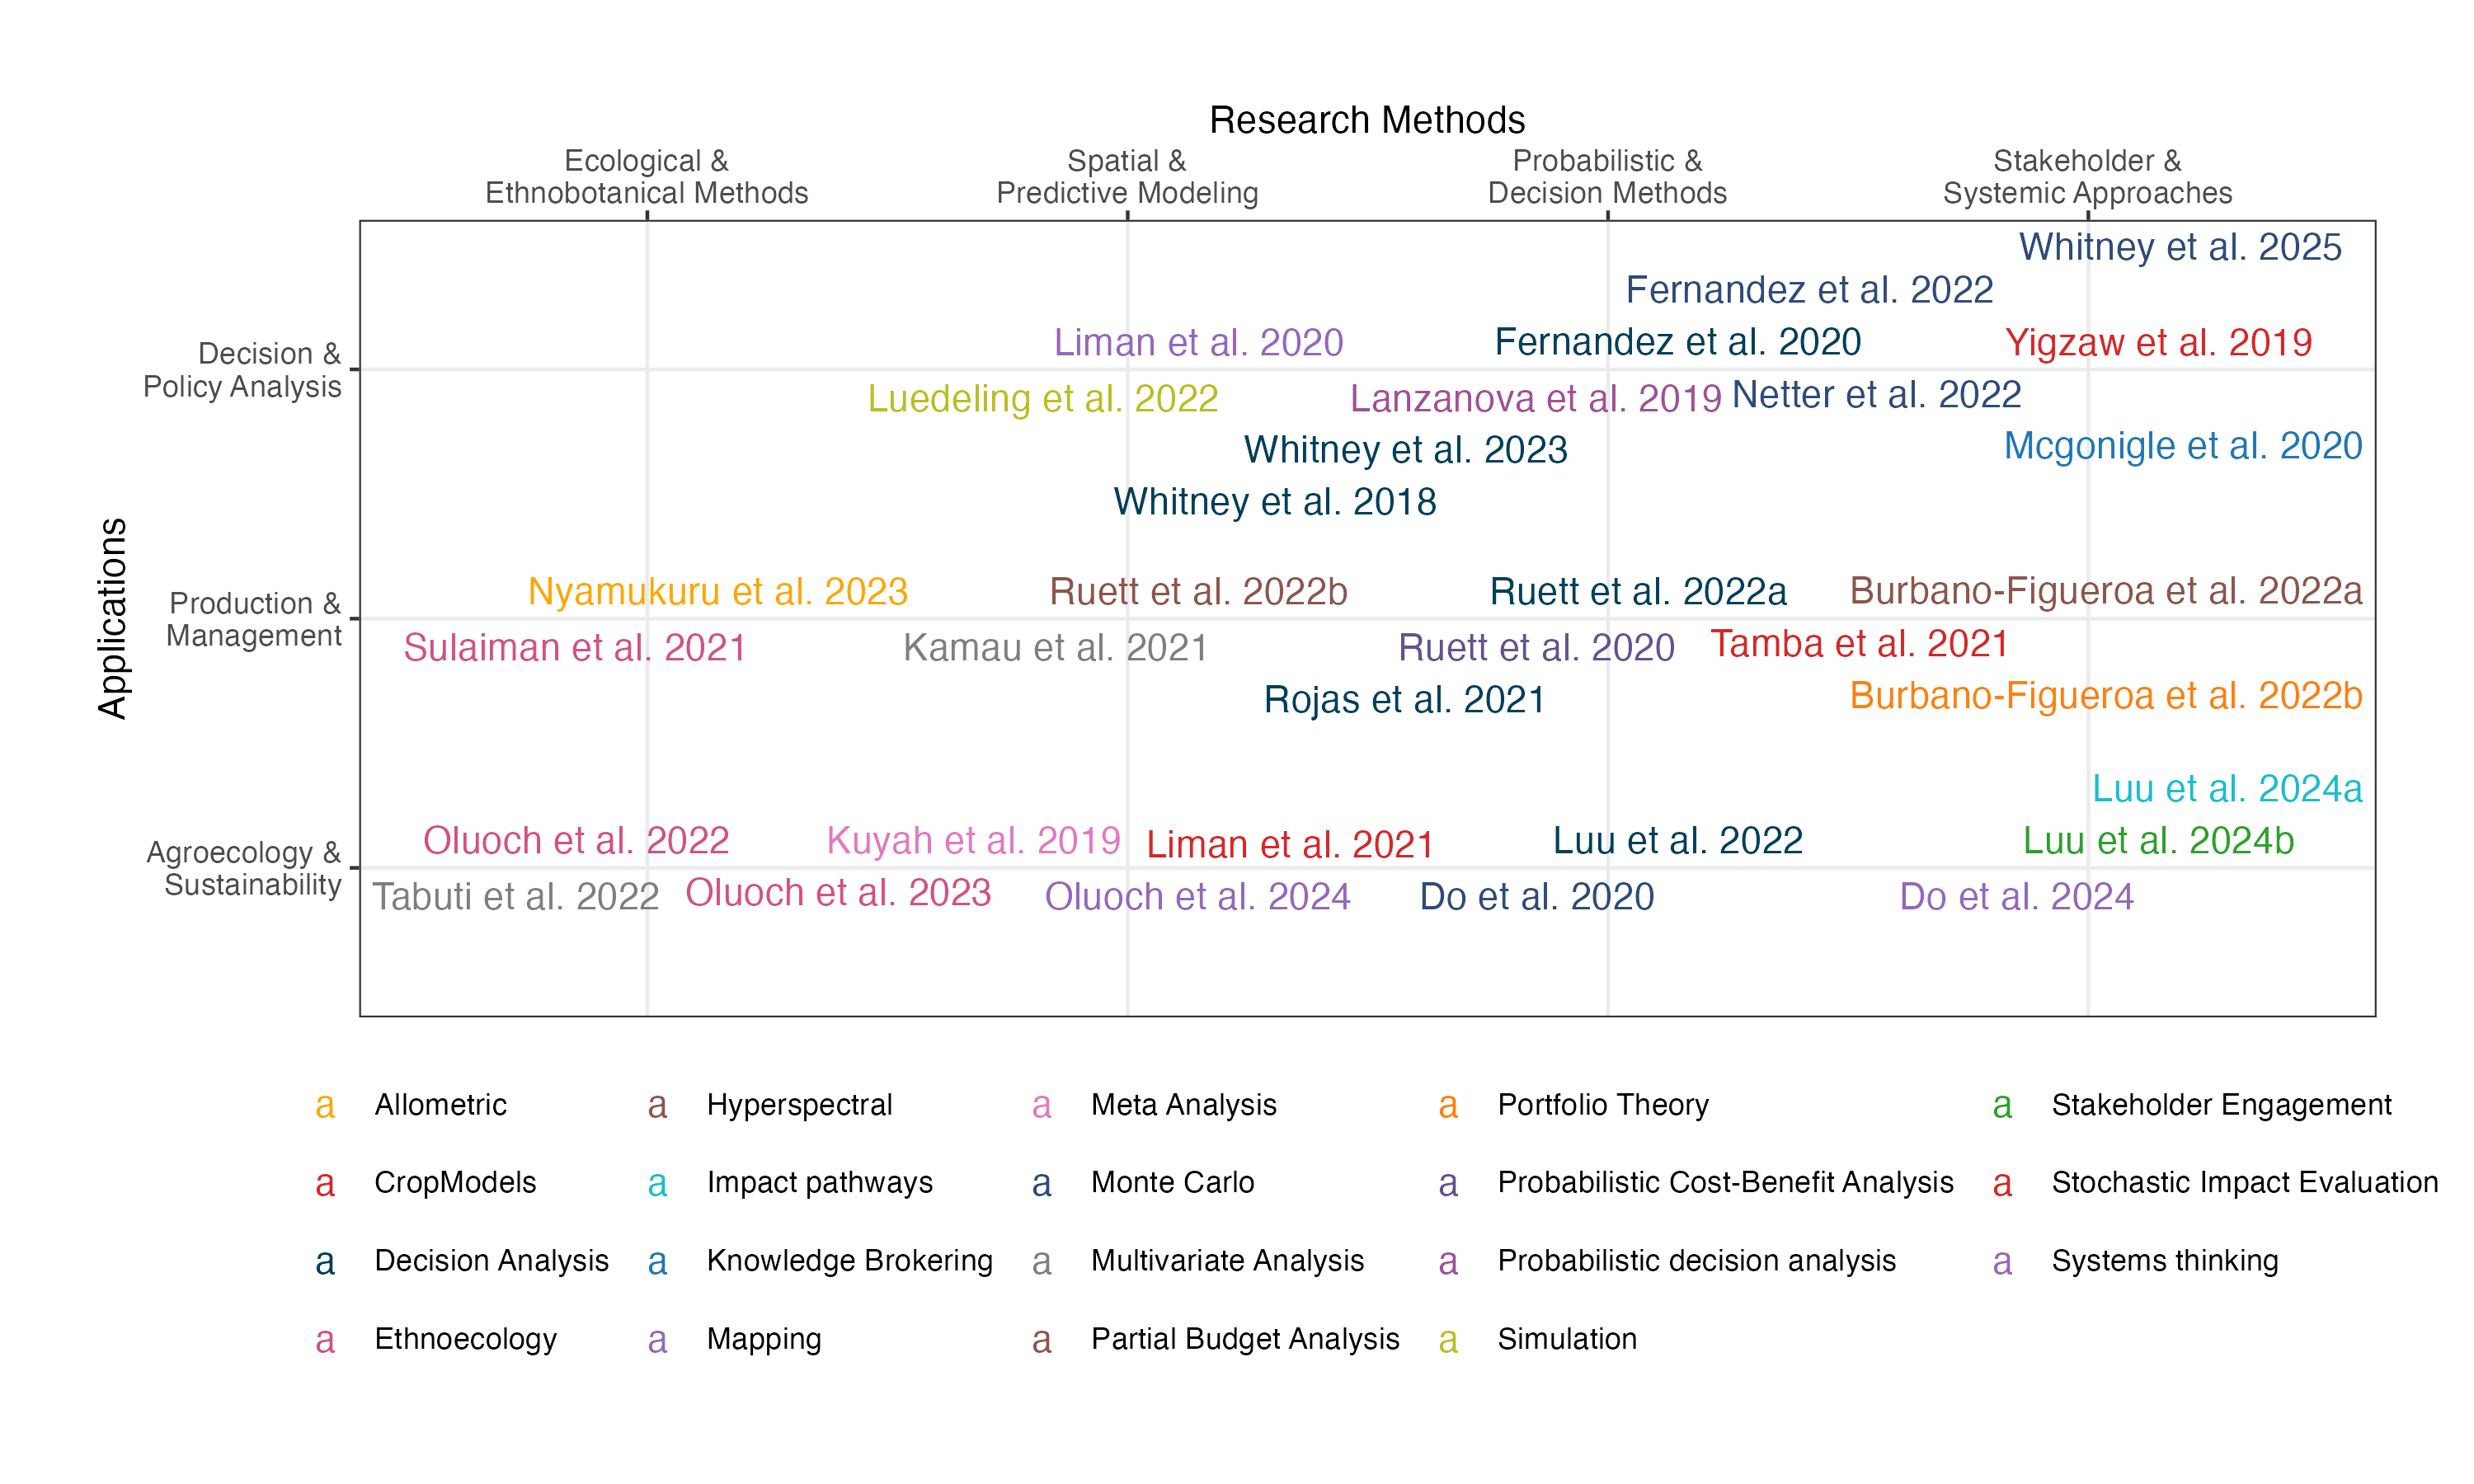
\includegraphics[width=1\linewidth,]{figures/scatter_plot_applications_methods} 

}

\caption{\label{fig:scatter_plot_applications_methods}Distribution of research contributions across methods and applications. The x-axis categorizes research methods, y-axis represents application areas, color-coded legend identifies the specific methodologies employed in each study.}\label{fig:scatter_plot_applications_methods}
\end{figure}

\end{landscape}

\newpage

\hypertarget{chapter_one}{%
\section{Advancing Agroecology through Decision Analytical
Methods}\label{chapter_one}}

Agricultural policy decisions have far-reaching consequences,
influencing both human nutrition and the sustainability of farming
systems. However, these decisions are often made under conditions of
profound uncertainty, where trade-offs between economic development,
ecological health, and social outcomes must be carefully negotiated.
Probabilistic decision tools provide a powerful framework for navigating
this complexity by enabling the evaluation of policy impacts while
accounting for uncertainty.

The integration of decision analytical methods into agroecology has not
only enhanced our understanding of these complex systems but also
provided actionable tools for practitioners and policymakers. In Ruett
\emph{et al.} (2020) we illustrate how decision analysis can inform pest
management strategies in ornamental horticulture, offering insights that
are directly applicable to horticulture systems. Furthermore, Netter
\emph{et al.} (2022) explores the application of these methods to carbon
offset projects, emphasizing the role of decision-support tools in
navigating trade-offs and uncertainties in agroforestry initiatives.

Through these contributions, my research underscores the transformative
potential of decision analytical methods in advancing agroecology. By
embracing complexity and integrating diverse perspectives, these tools
provide a foundation for designing agricultural systems that are
resilient, equitable, and aligned with the principles of sustainable
development. This work not only advances the theoretical understanding
of agroecology but also bridges the gap between research and practice,
empowering stakeholders to make informed decisions in the face of
uncertainty.

Together, these studies demonstrate the transformative potential of
decision analysis in optimizing both horticultural and agroforestry
systems. By addressing risks, uncertainties, and trade-offs, these tools
contribute to sustainable agricultural landscapes that support economic
viability, environmental health, and social well-being. This integration
aligns with global sustainability goals, emphasizing the need for
robust, evidence-based decision-making frameworks.

Decision analytical methods are critical in advancing agroecology and
addressing the pressing challenges of sustainable development. By
embracing complexity and uncertainty, these methods provide robust
frameworks for evaluating interventions, optimizing resource use, and
balancing trade-offs across ecological, economic, and social dimensions.
Through applications ranging from agroforestry adoption in Vietnam to
pest management in horticulture and carbon offset initiatives, my
research demonstrates the versatility and power of probabilistic tools
and participatory modeling. These approaches not only improve the
scientific rigor of decision-making but also ensure that interventions
are relevant, equitable, and aligned with the needs of local
communities.

The demand for scalable and adaptable tools is becoming more urgent as
the world faces growing pressures from climate change, resource
scarcity, and population growth. Decision analytical methods offer a
pathway to navigate these challenges, enabling stakeholders to make
informed choices that promote resilience, sustainability, and equity.
The future of agroecology and sustainable development lies in
integrating diverse knowledge systems, fostering collaboration across
disciplines, and refining tools that bridge the gap between research and
practice. By continuing to innovate and expand the use of decision
analysis in agricultural contexts, we can contribute to building a more
sustainable and equitable global food system.

Probabilistic decision tools can effectively link agricultural policy
with nutritional outcomes. Unlike deterministic models, which assume
fixed outcomes, probabilistic approaches explicitly account for
uncertainty, enabling robust and flexible decision-making. This is
particularly important in contexts like Uganda, where data availability
is limited, and policy decisions must balance competing priorities. The
studies demonstrate the potential of probabilistic tools to illuminate
the trade-offs and synergies within agricultural systems. By combining
empirical evidence with expert insights, we provided policymakers with
actionable recommendations to design interventions that not only drive
economic growth but also safeguard nutrition and food security. The
methods have broader applicability beyond Uganda. Probabilistic decision
tools can be adapted to diverse agricultural contexts, offering a
scalable approach to evaluating the impacts of policies on nutrition,
livelihoods, and sustainability. By bridging the gap between policy
aspirations and on-the-ground realities, these tools contribute to a
holistic understanding of agricultural systems and their role in
advancing sustainable development.

\hypertarget{applying-structured-decision-models}{%
\subsection{Applying Structured Decision
Models}\label{applying-structured-decision-models}}

In Whitney \emph{et al.} (2018b)
\protect\hyperlink{whitney_probabilistic_2018}{Paper 1}, my co-authors
and I explored the application of structured decision analysis for
supporting interventions to agroecological systems. By employing
probabilistic modeling, we demonstrated how these tools could optimize
outcomes across multiple dimensions, including ecological conservation,
economic resilience, and human well-being. This work highlighted the
value of integrating diverse data sources and stakeholder inputs into
decision models, ensuring that the solutions are both scientifically
robust and contextually relevant. The work defined and demonstrated a
set of methods for working with expert groups to define causal model
structures for development decisions (Fig.
\ref{fig:workshop_model_development}).

\begin{figure}[H]

{\centering 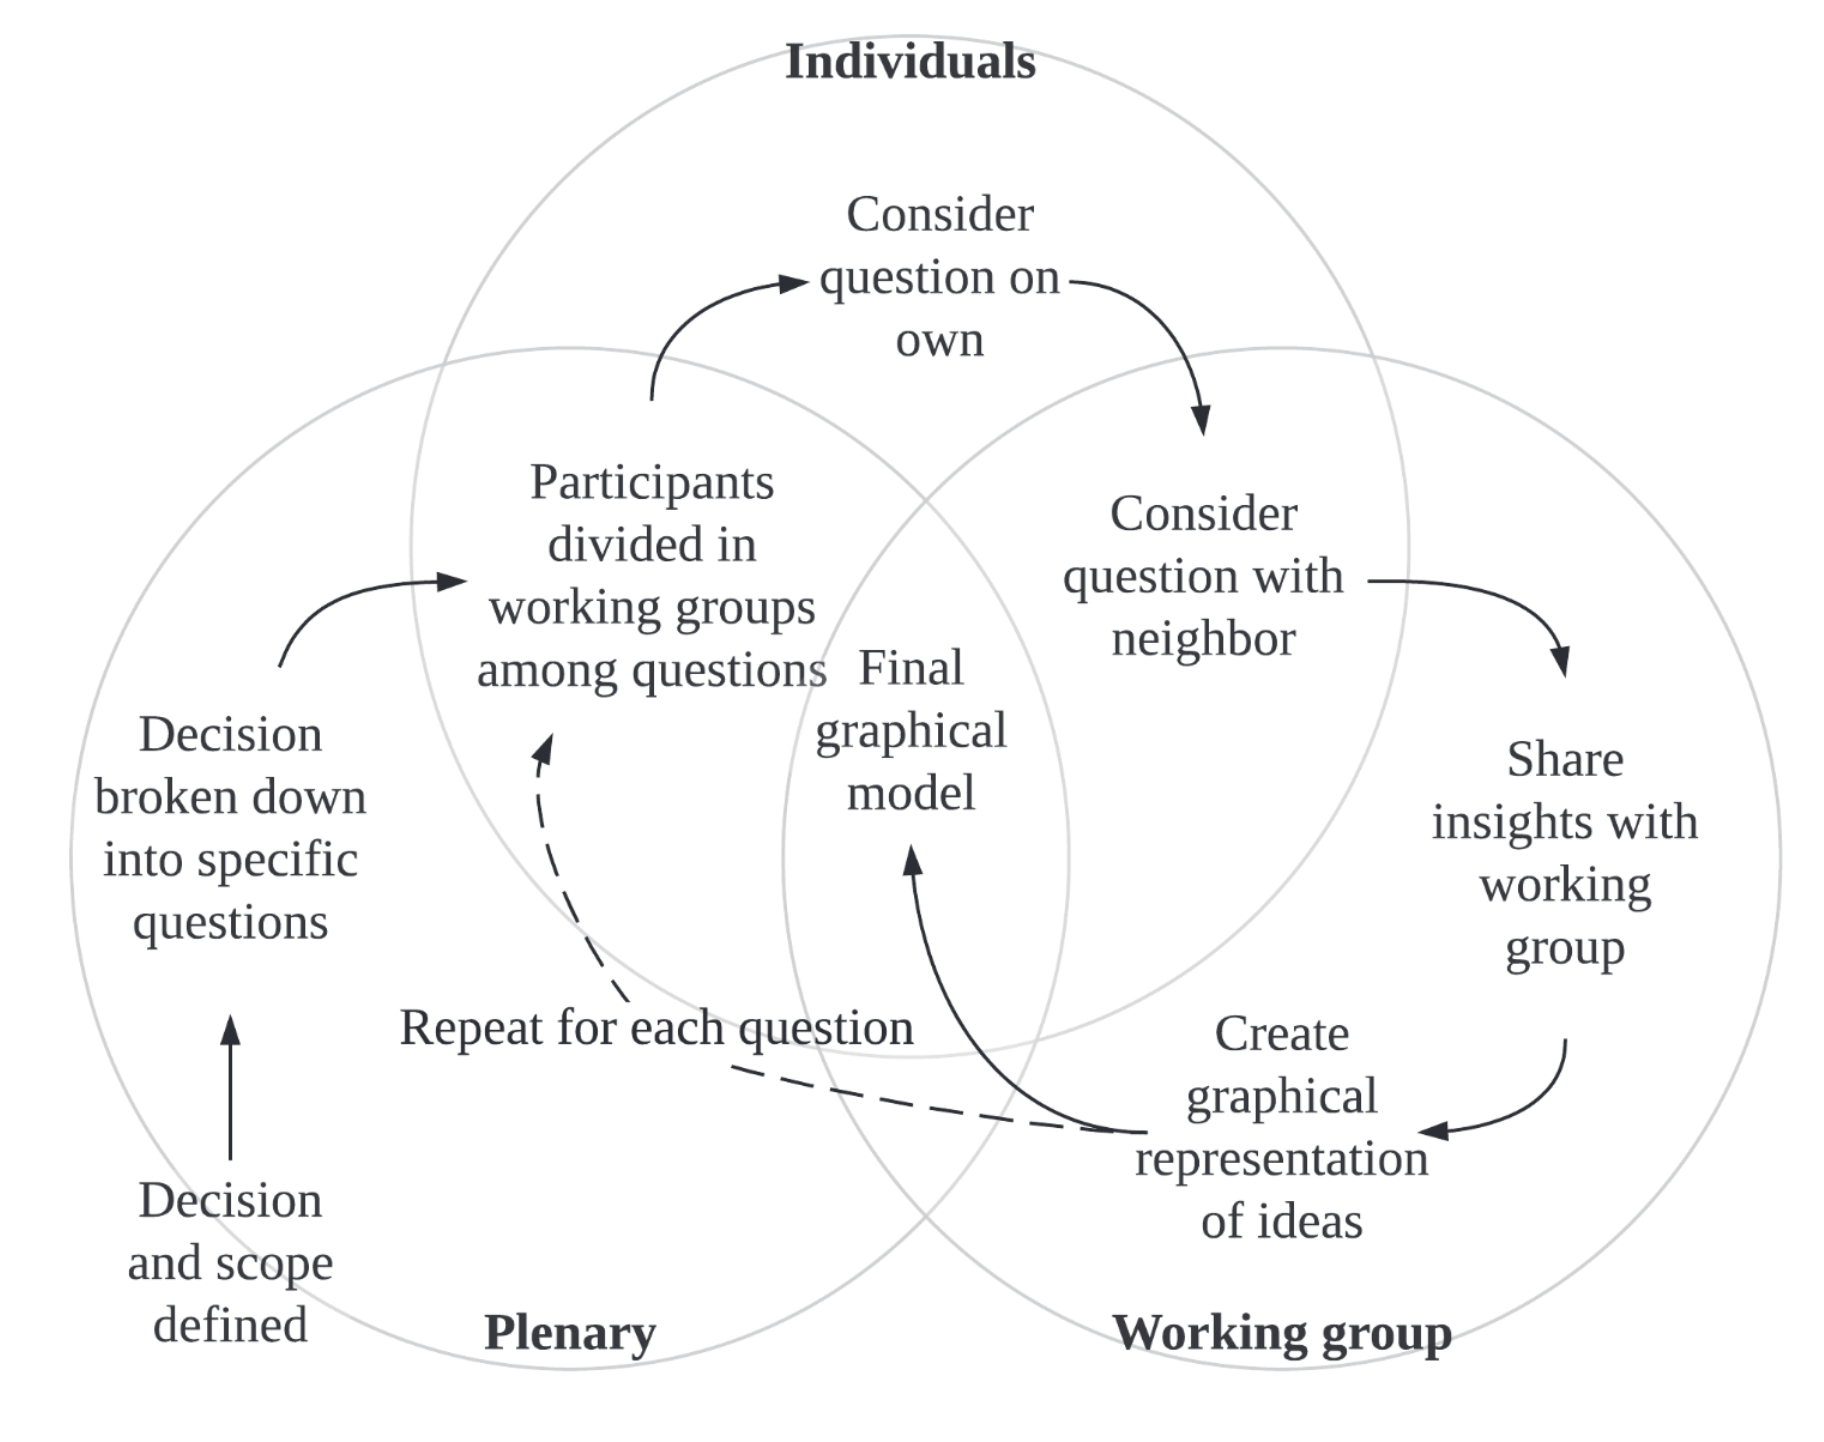
\includegraphics[width=0.6\linewidth,]{figures/workshop_model_development} 

}

\caption{\label{fig:Figures/workshop_model_development}Process used for eliciting graphical representations of decisions from expert groups (Whitney et al. 2018).}\label{fig:Figures/workshop_model_development}
\end{figure}

To simplify the task of constructing Bayesian Networks from these causal
models we also designed innovative ways to fill the often very complex
conditional probability tables with expert elicited probabilities. We
used a likelihood method to elicit influence weights rather than whole
tables of probabilities. We asked experts to provide a typical
distribution of each variable as well as the response and a weighting
factor for each state of the child node and each state of the parent
nodes (Fig. \ref{fig:node_states_cpts}).

\begin{figure}[H]

{\centering 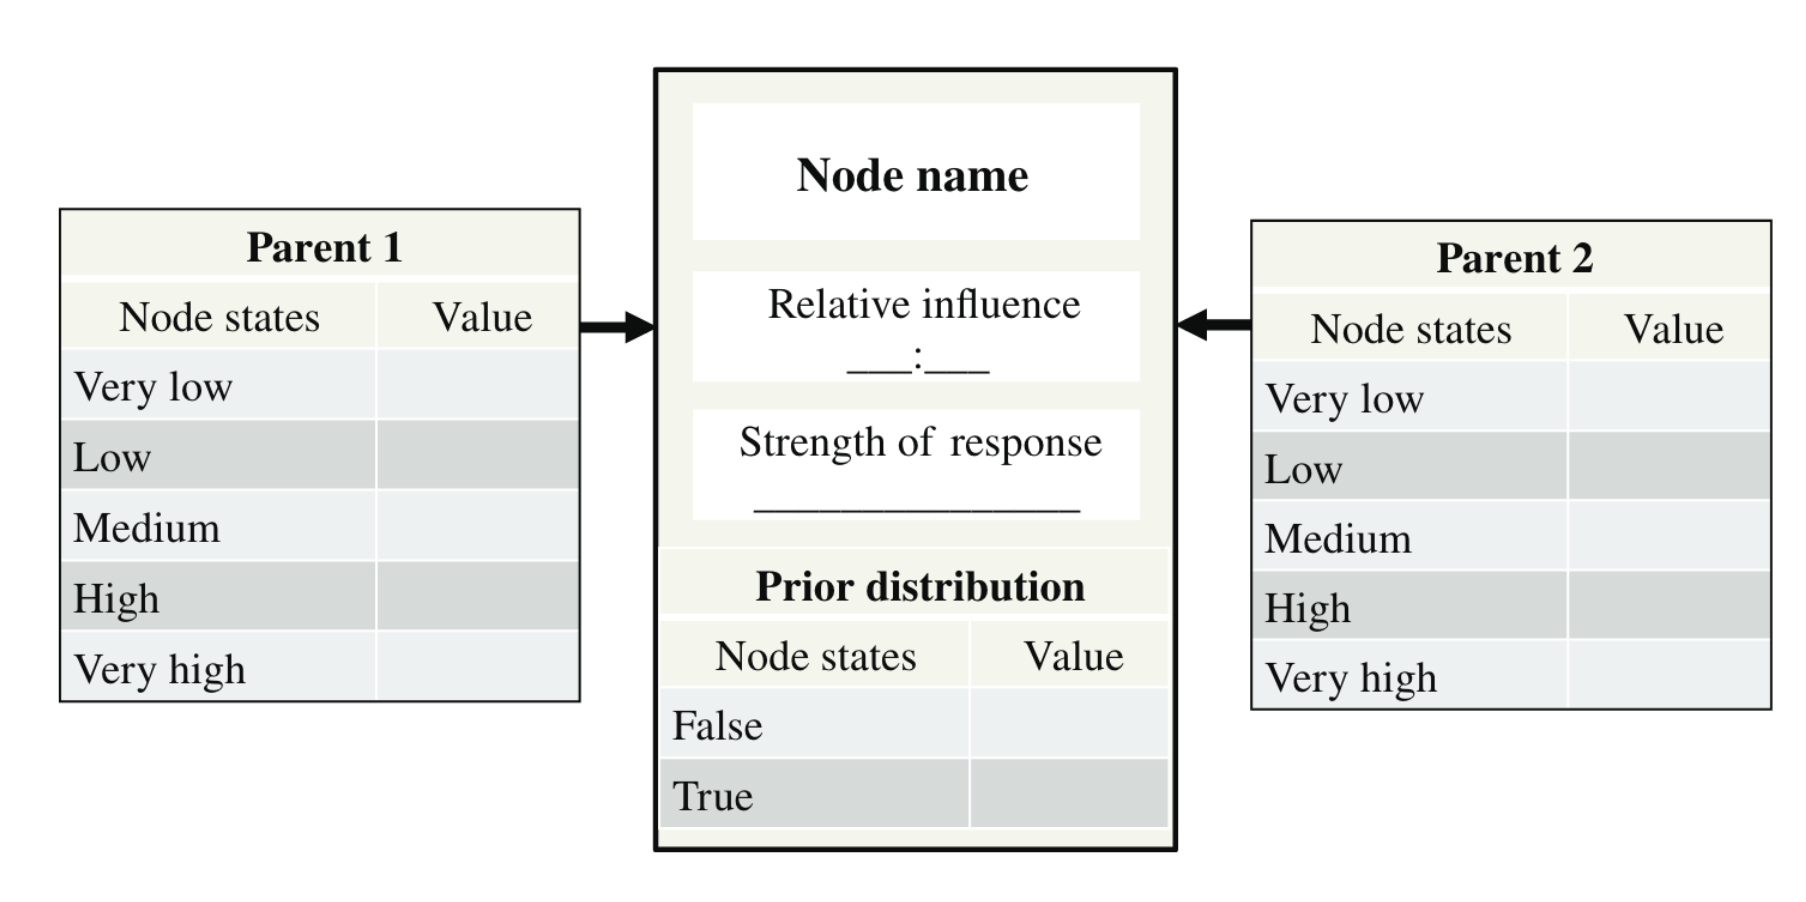
\includegraphics[width=0.8\linewidth,]{figures/node_states_cpts} 

}

\caption{\label{fig:node_states_cpts}Tool for expert-informed Conditional Probability Table (CPT) for use in a Bayesian Network (Whitney et al. 2018).}\label{fig:node_states_cpts}
\end{figure}

In Whitney \emph{et al.} (2018b), we explored the application of the
resulting Bayesian Networks as a decision-support tool for agricultural
policy analysis (Fig. \ref{fig:vision_2040_bn}). This study focused on
Uganda's Vision 2040, an ambitious development strategy aimed at
transforming the country's agricultural landscape from subsistence
farming to large-scale commercial agriculture. While this vision
promised economic growth, its potential impacts on rural livelihoods and
household nutrition were largely uncertain.

\begin{landscape}

\begin{figure}[H]

{\centering 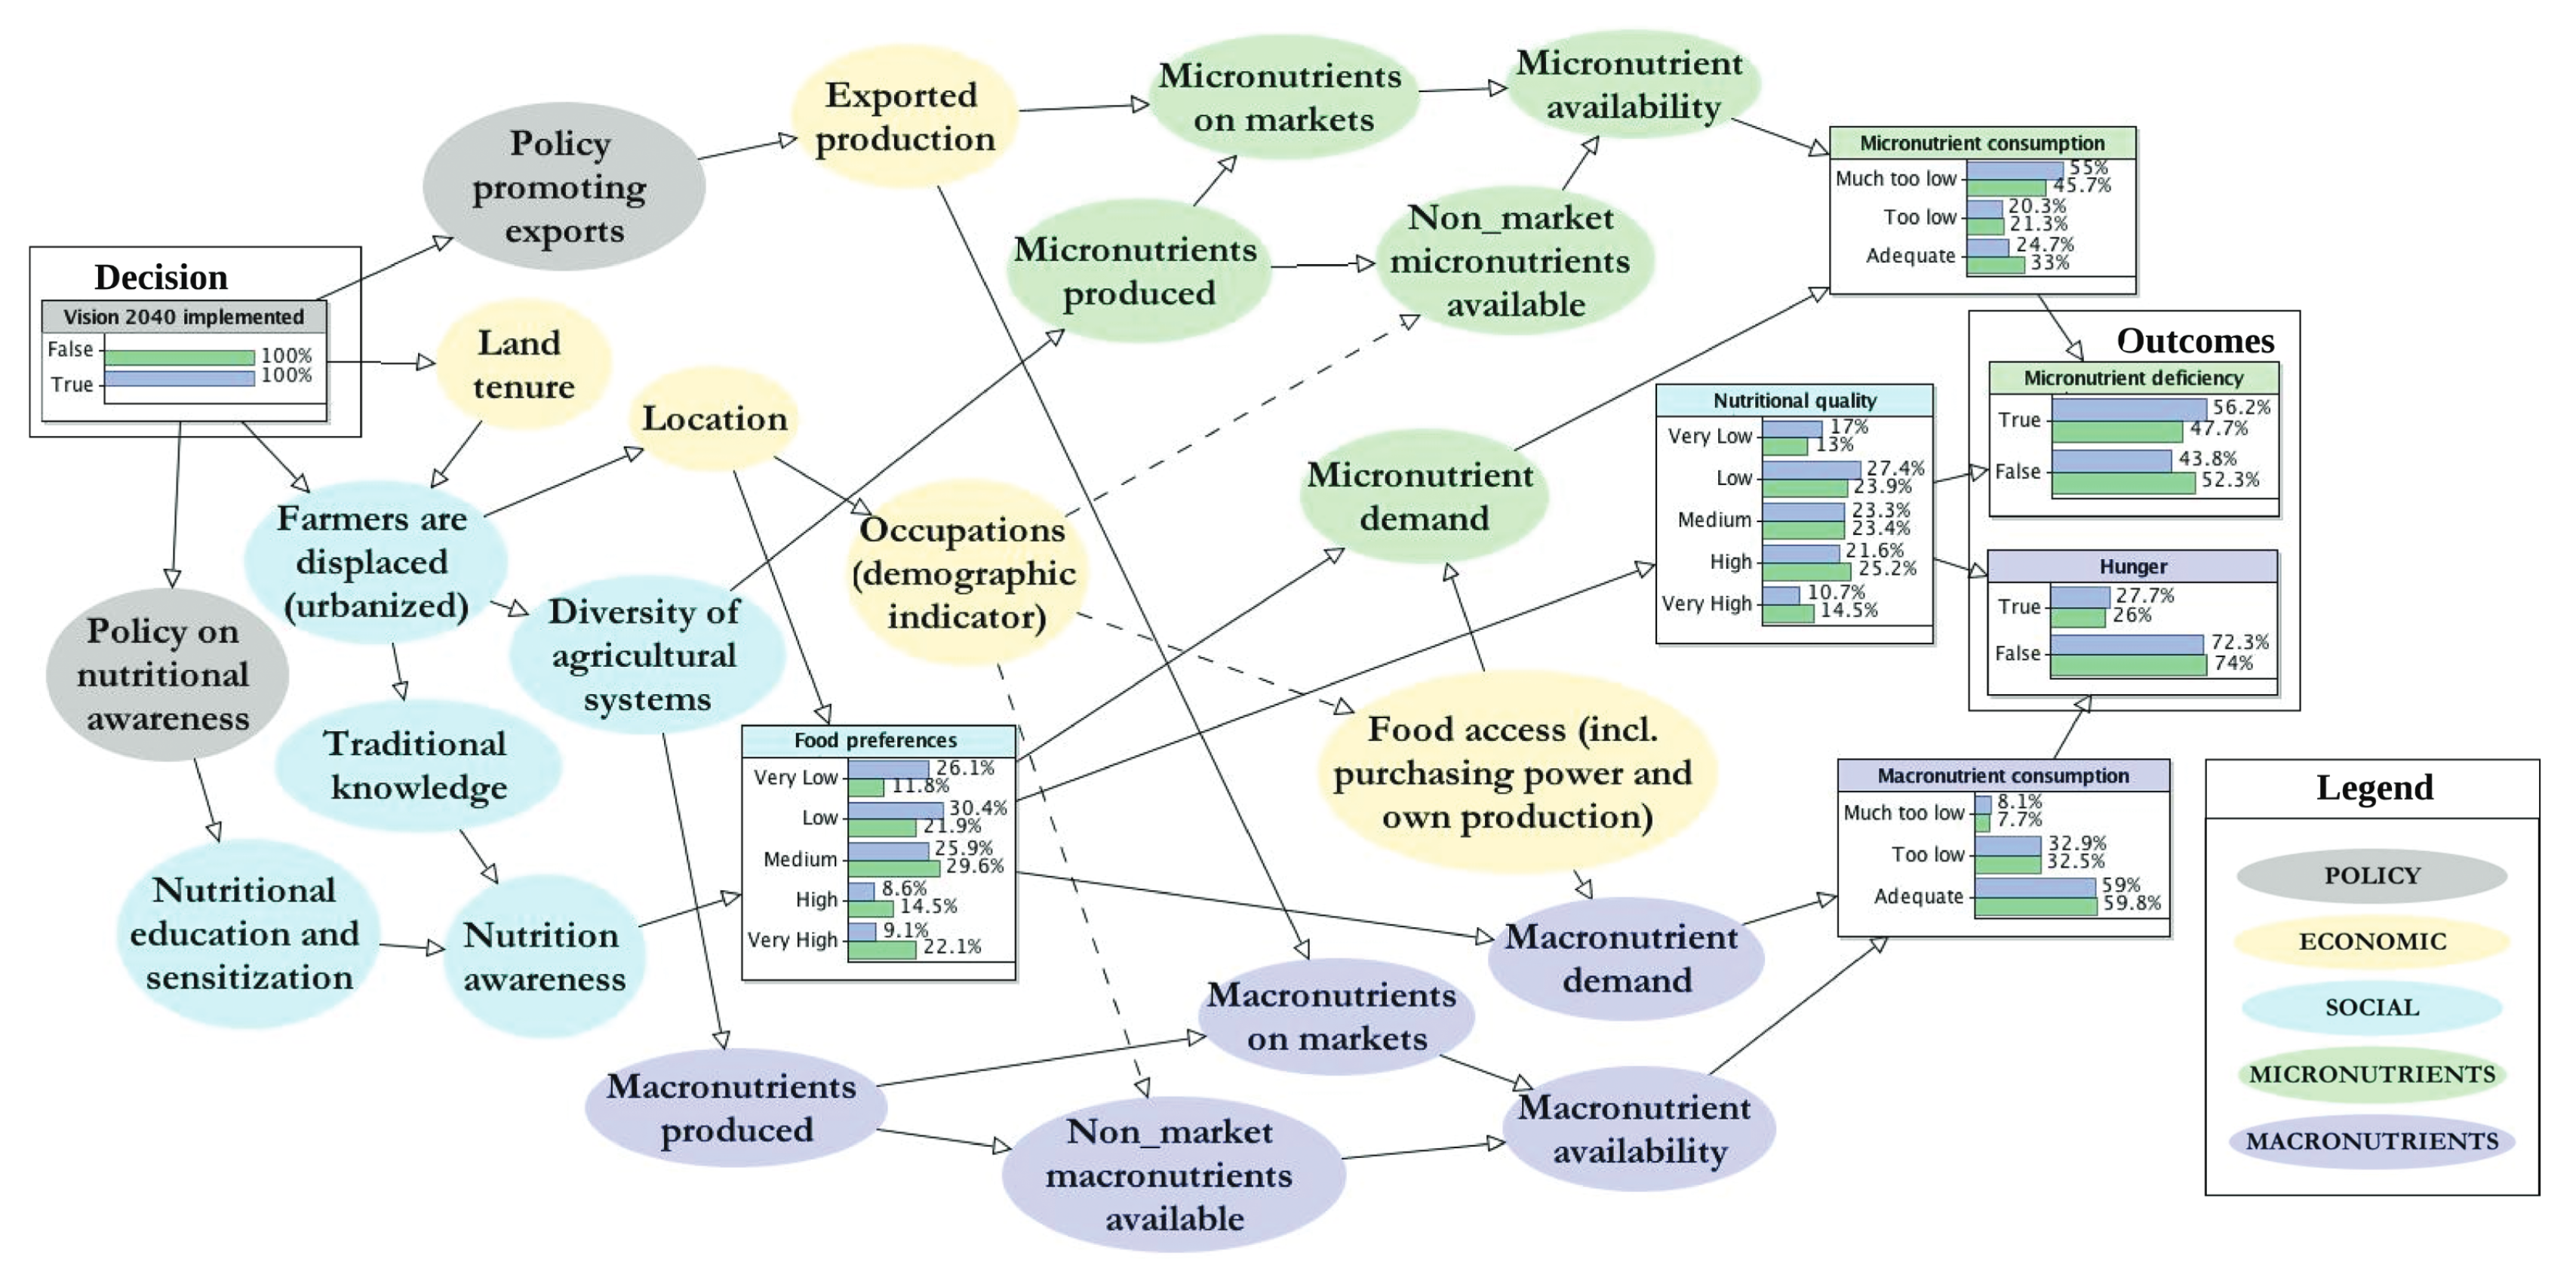
\includegraphics[width=1\linewidth,]{figures/vision_2040_bn} 

}

\caption{\label{fig:vision_2040_bn}Bayesian Network (BN) for impact of Vision 2040 on household nutrition in Uganda. (Whitney et al. 2018)}\label{fig:vision_2040_bn}
\end{figure}

In Figure \ref{fig:vision_2040_bn} probabilities are shown (boxes) for outcome variables and variables with the highest value of information. Green bars show the probabilities for the node states for the scenario that the Vision 2040 decision is not implemented (“Vision 2040 false”), and blue bars show probabilities for the scenario that the Vision 2040 decision is implemented (“Vision 2040 true”)

\end{landscape}

We modeled the causal pathways between agricultural interventions and
their nutritional outcomes. By integrating empirical data with expert
knowledge, we were able to quantify the probabilities of various
outcomes, providing a nuanced understanding of the trade-offs inherent
in Uganda's agricultural transformation strategy. This approach allowed
us to explore critical questions, such as how shifts in land use and
farming practices might affect household access to nutritious foods and
the prevalence of micronutrient deficiencies.

A key innovation in this work was the ability to represent complex
interdependencies within agricultural systems. This study linked policy
interventions to nutrition outcomes, emphasizing stochastic modeling's
role in identifying trade-offs and mitigating unintended consequences.
For instance, while Vision 2040 aimed to boost economic productivity
through large-scale farming, our model revealed potential risks,
including reduced access to diverse and nutrient-rich foods for rural
households. The results suggested that the policy could inadvertently
exacerbate micronutrient deficiencies, even as it achieved its economic
objectives.

By performing sensitivity analysis, we identified the factors with the
greatest influence on nutritional outcomes, such as dietary diversity
and market access. Additionally, the use of value of information (VOI)
analysis highlighted areas where targeted data collection could
significantly improve decision-making. These insights provided a roadmap
for policymakers to mitigate negative outcomes while pursuing
development goals (Fig. \ref{fig:vision_2040_voi}).

\begin{figure}[h]
  \centering
  \begin{minipage}{0.6\textwidth}
    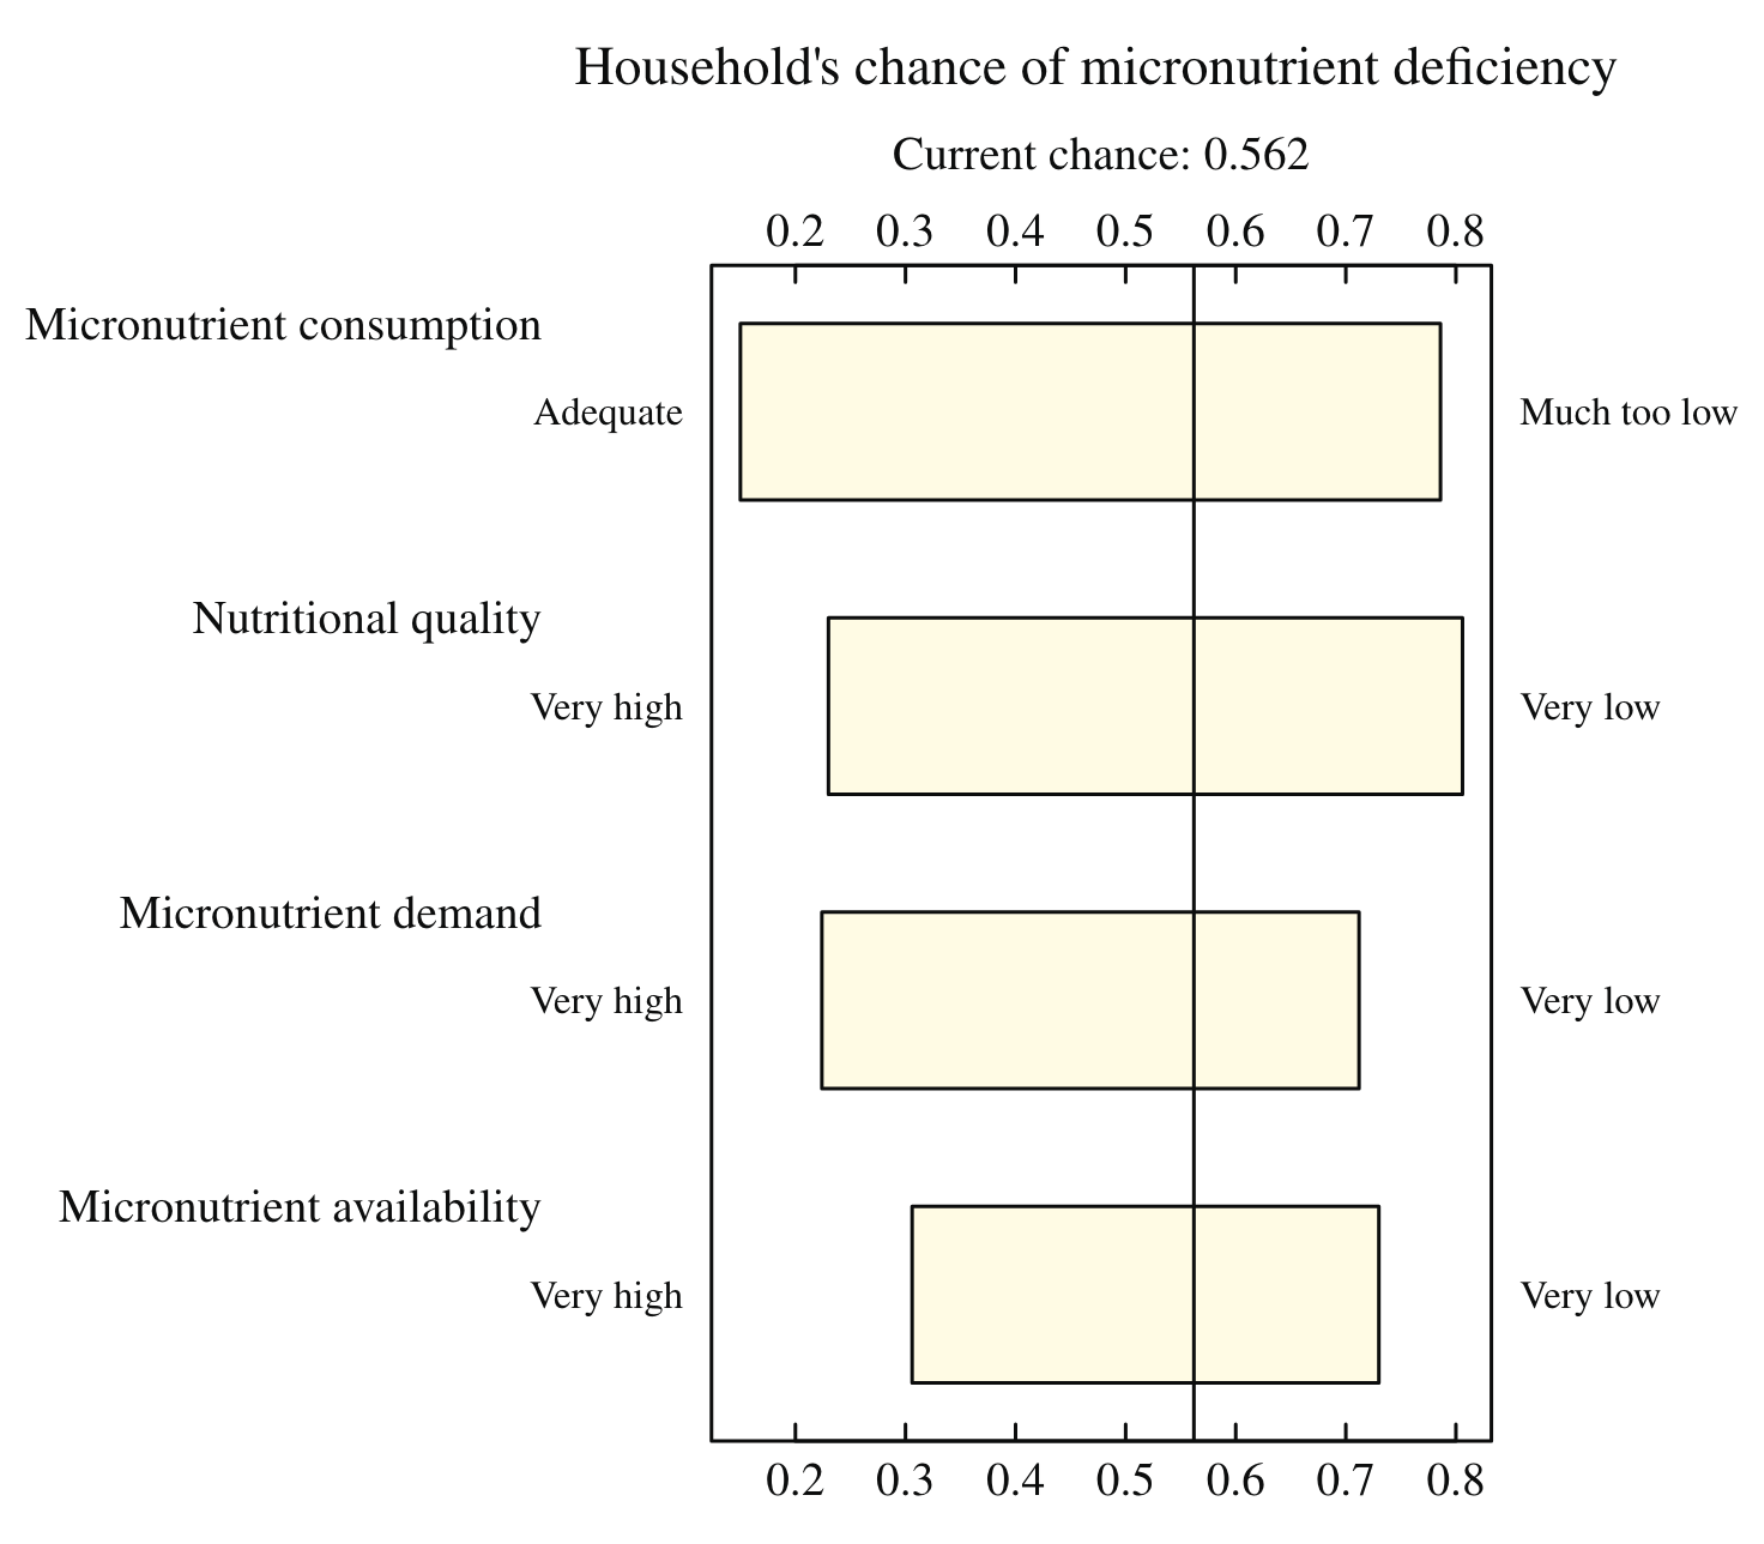
\includegraphics[width=\textwidth]{figures/vision_2040_voi.png}
  \end{minipage}%
  \begin{minipage}{0.35\textwidth}
    \caption{\label{fig:vision_2040_voi}Sensitivity analysis of a Bayesian Network for the probability of household micronutrient deficiency within 10 years of the implementation of Uganda's Vision 2040 (Whitney et al. 2018).}
  \end{minipage}
\end{figure}

A key contribution of my research has been the development and
application of decision analysis frameworks tailored to the complexities
of agroecological systems. Unlike conventional models that prioritize
narrow objectives, such as maximizing crop yield, my work adopts a
systems-level perspective. In Whitney \emph{et al.} (2018b), I
demonstrated how probabilistic decision tools could evaluate the
trade-offs of Uganda's Vision 2040 policy, revealing unintended
consequences on rural livelihoods. This study underscores the value of
integrating diverse information sources, stakeholder knowledge, and
probabilistic methods to guide decision-making around development
interventions.

Building on this, we extended probabilistic decision analysis to
reservoir sedimentation management in Burkina Faso (Lanzanova \emph{et
al.} 2019). Using Monte Carlo simulations, the study evaluated
interventions aimed at mitigating sedimentation risks, identifying the
most effective strategies for maintaining agricultural water storage
capacity (Fig. \ref{fig:lanzanov_protocol}).

\begin{landscape}

\begin{figure}[H]

{\centering 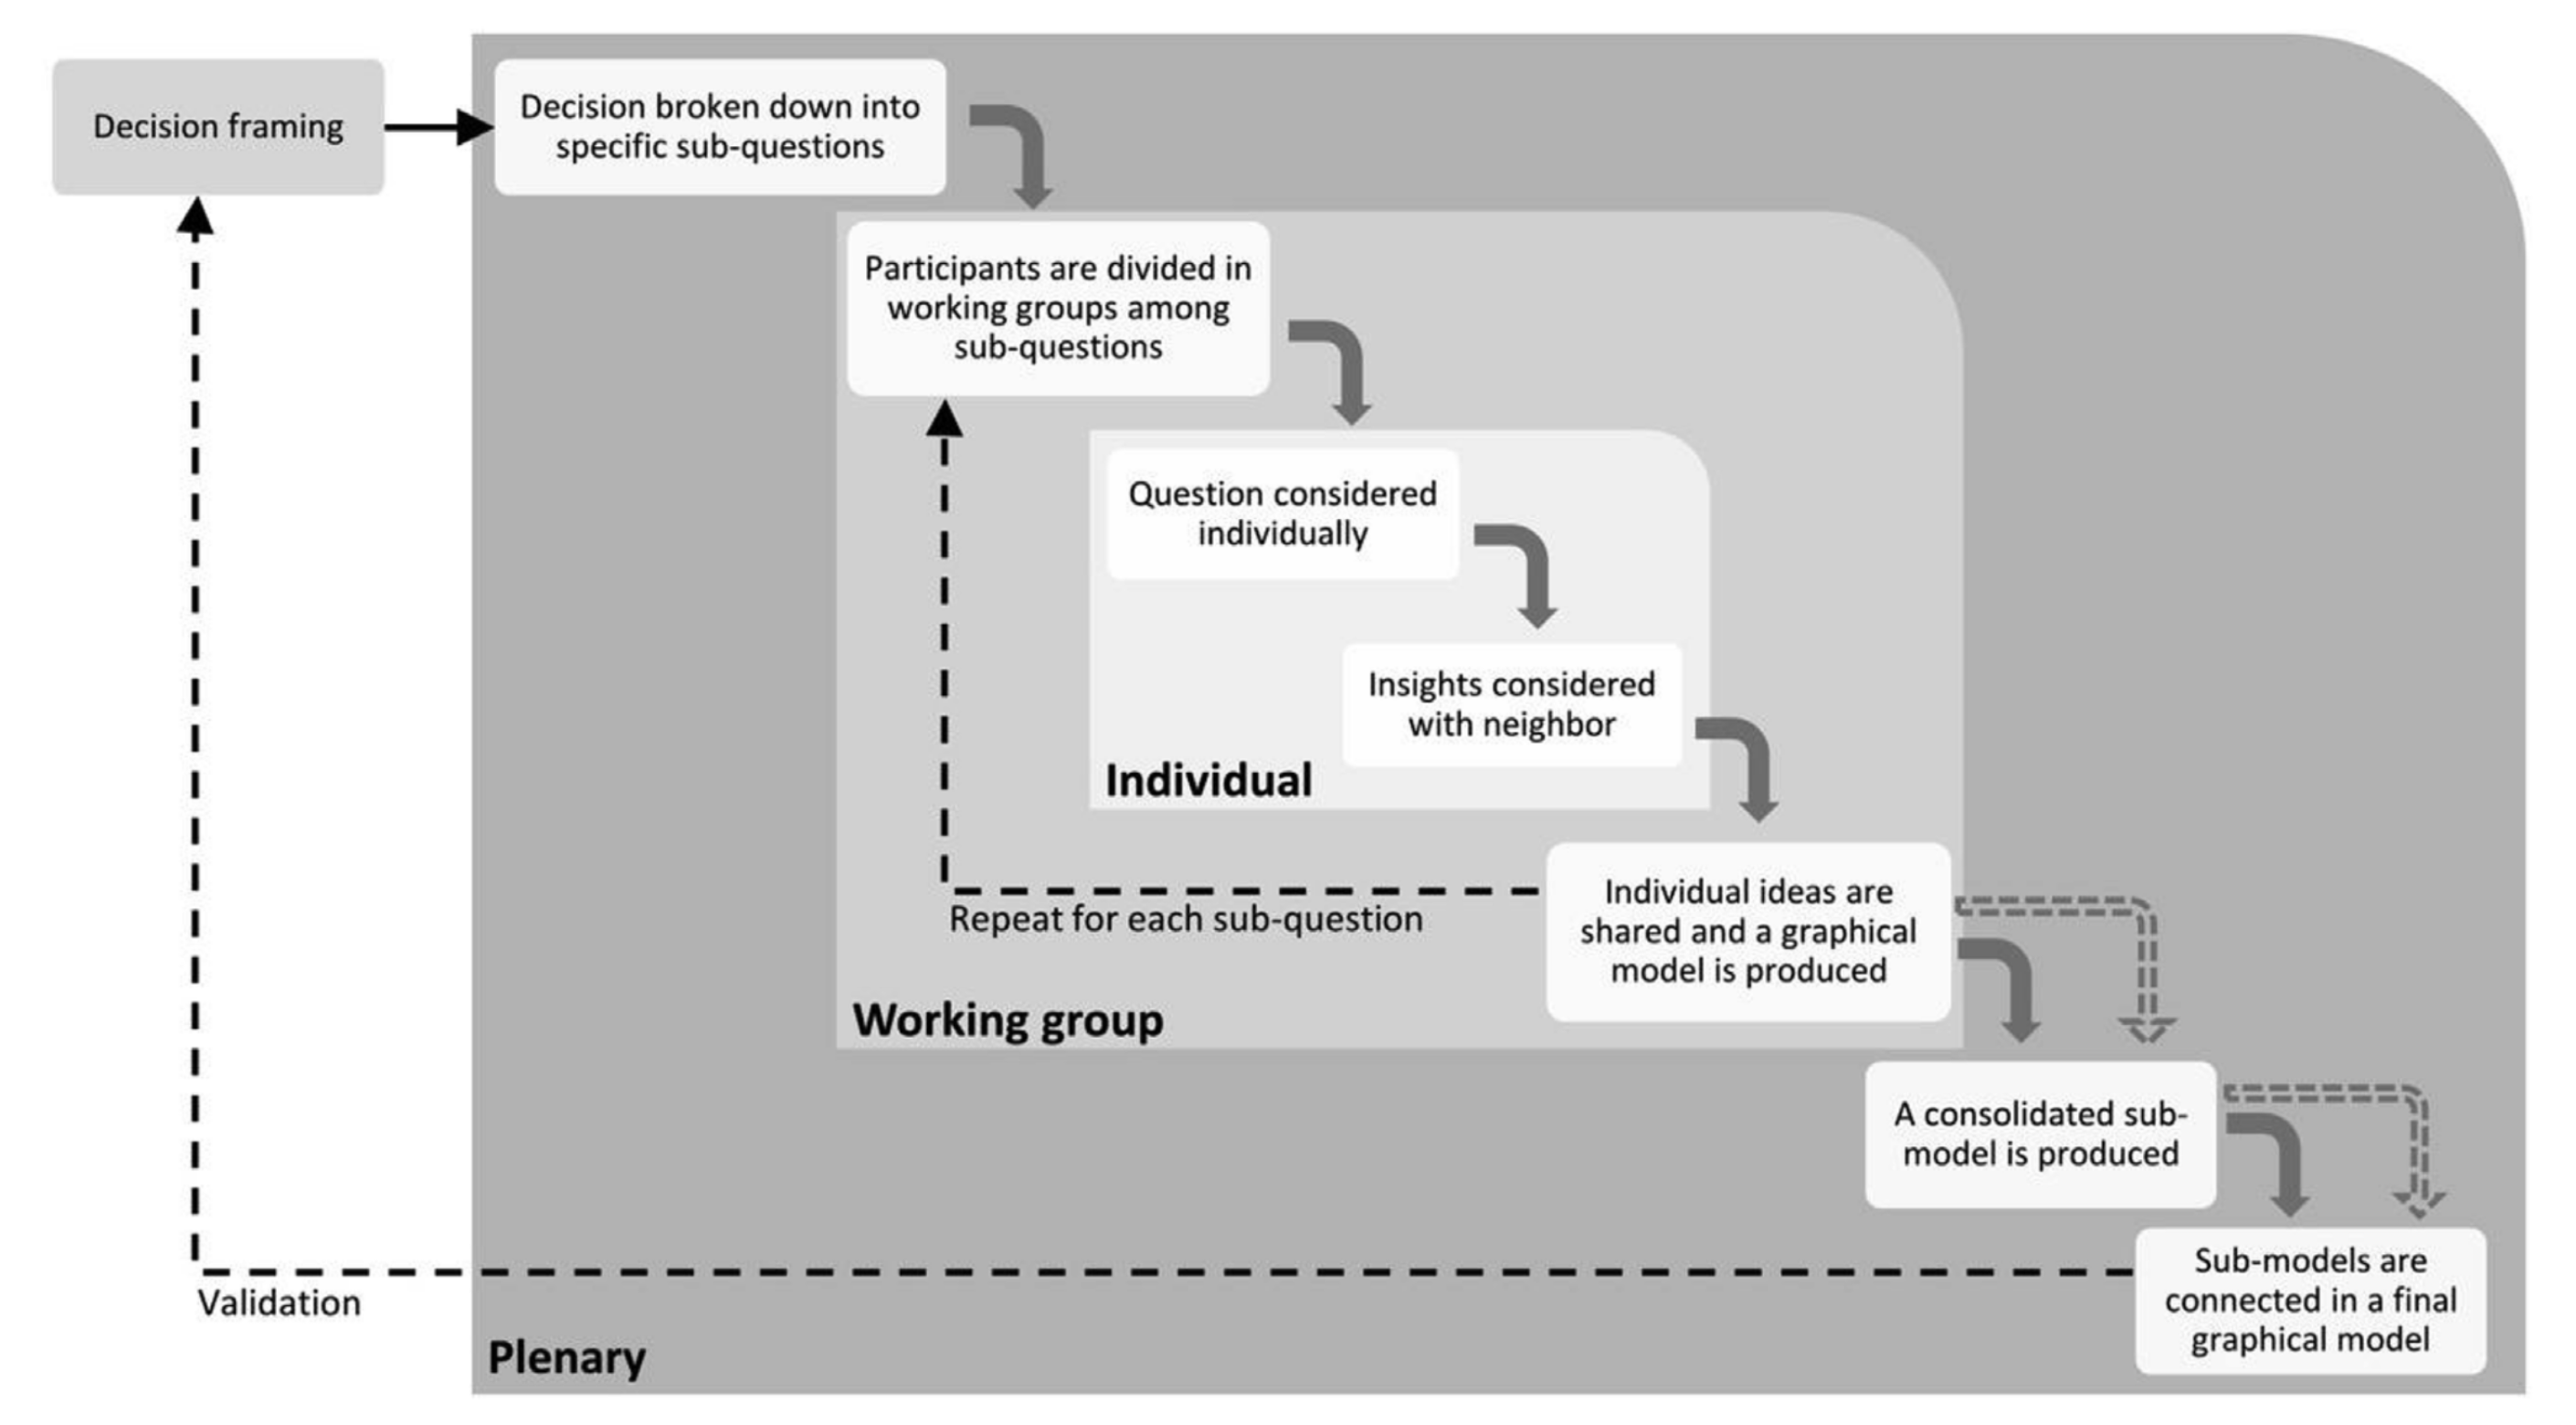
\includegraphics[width=1\linewidth,]{figures/lanzanov_protocol} 

}

\caption{\label{fig:lanzanov_protocol}Diagram of a four-stage protocol for eliciting expert knowledge for sedimentation risk reduction in Burkina Faso (Lanzanova et al. 2019)}\label{fig:lanzanov_protocol}
\end{figure}

\end{landscape}

Expanding methods for decision structuring and model development (Fig.
\ref{fig:lanzanov_protocol}), the analysis combined Monte Carlo
simulation, Partial Least Squares regression, and Value of Information
analysis to quantify intervention trade-offs. The study demonstrated how
probabilistic modeling supports robust decision-making under
uncertainty, showing that a combination of dredging, rock dams, and
buffer schemes offers the highest probability of sustaining agricultural
production (Lanzanova \emph{et al.} 2019)
\protect\hyperlink{lanzanova_improving_2019}{Paper 10}.

Further expanding on stochastic modeling, Yigzaw \emph{et al.} (2019)
applied Stochastic Impact Evaluation (SIE) to assess the feasibility of
irrigation dams in Tigray, Ethiopia. The study incorporated
expert-elicited probabilities within a probabilistic decision framework,
evaluating potential benefits, costs, and risks of large-scale
irrigation investments. Our application of these methods provided
probabilistic estimates of hydrological, economic, and environmental
trade-offs, supporting climate-resilient water management strategies.
One of the key innovations in the work is the structured use of expert
knowledge within Monte Carlo simulations and Partial Least Squares
analysis, demonstrating how uncertainty quantification enhances
decision-support systems. The findings highlight the role of
probabilistic modeling in formalizing diverse expert perspectives,
revealing trade-offs, and integrating uncertainty into agricultural
water management strategies (Yigzaw \emph{et al.} 2019)
\protect\hyperlink{yigzaw_stochastic_2019}{Paper 11}.

\hypertarget{addresssing-complexity-and-uncertainty-in-agroforestry-interventions}{%
\subsection{Addresssing Complexity and Uncertainty in Agroforestry
Interventions}\label{addresssing-complexity-and-uncertainty-in-agroforestry-interventions}}

Agroforestry, the deliberate integration of woody perennials into
agricultural systems, offers a compelling approach to sustainable
agricultural development, particularly in regions facing environmental
and socio-economic pressures. By enhancing multiple ecosystem
services---including provisioning, regulating, and supporting
functions---agroforestry can improve both food security and climate
resilience. However, managing agricultural landscapes for sustainability
requires balancing trade-offs, as efforts to maximize provisioning
services can sometimes diminish regulating and maintenance functions.

Our meta-analysis in Kuyah \emph{et al.} (2019) demonstrates that
agroforestry systems in sub-Saharan Africa can increase crop yields
while simultaneously improving soil fertility, reducing erosion, and
enhancing water regulation. These systems contribute to higher levels of
total soil nitrogen, organic carbon, and phosphorus while mitigating
runoff and soil loss. However, these benefits are highly
context-dependent, shaped by ecological conditions, management
strategies, and species selection. We performed a meta-analysis of
agroforestry vs.~non-agroforestry effects on provisioning of ecosystem
services across sub-Saharan Africa (Fig.
\ref{fig:kuyah_agroforestry_violin}). We used bootstrapped t0 values of
agroforestry minus non-agroforestry effects. RR \textless{} 1 and RR
\textgreater{} 1 with (\%) observations below or above 1 respectively.
Values in brackets indicate the number of studies reviewed (N) and
observations (NO). We synthesized evidence of ecosystem service benefits
and productivity gains (Kuyah \emph{et al.} 2019). Agroforestry
increased crop yields, soil nutrients, and water retention while
reducing runoff and soil loss.

\begin{landscape}

\begin{figure}[H]

{\centering 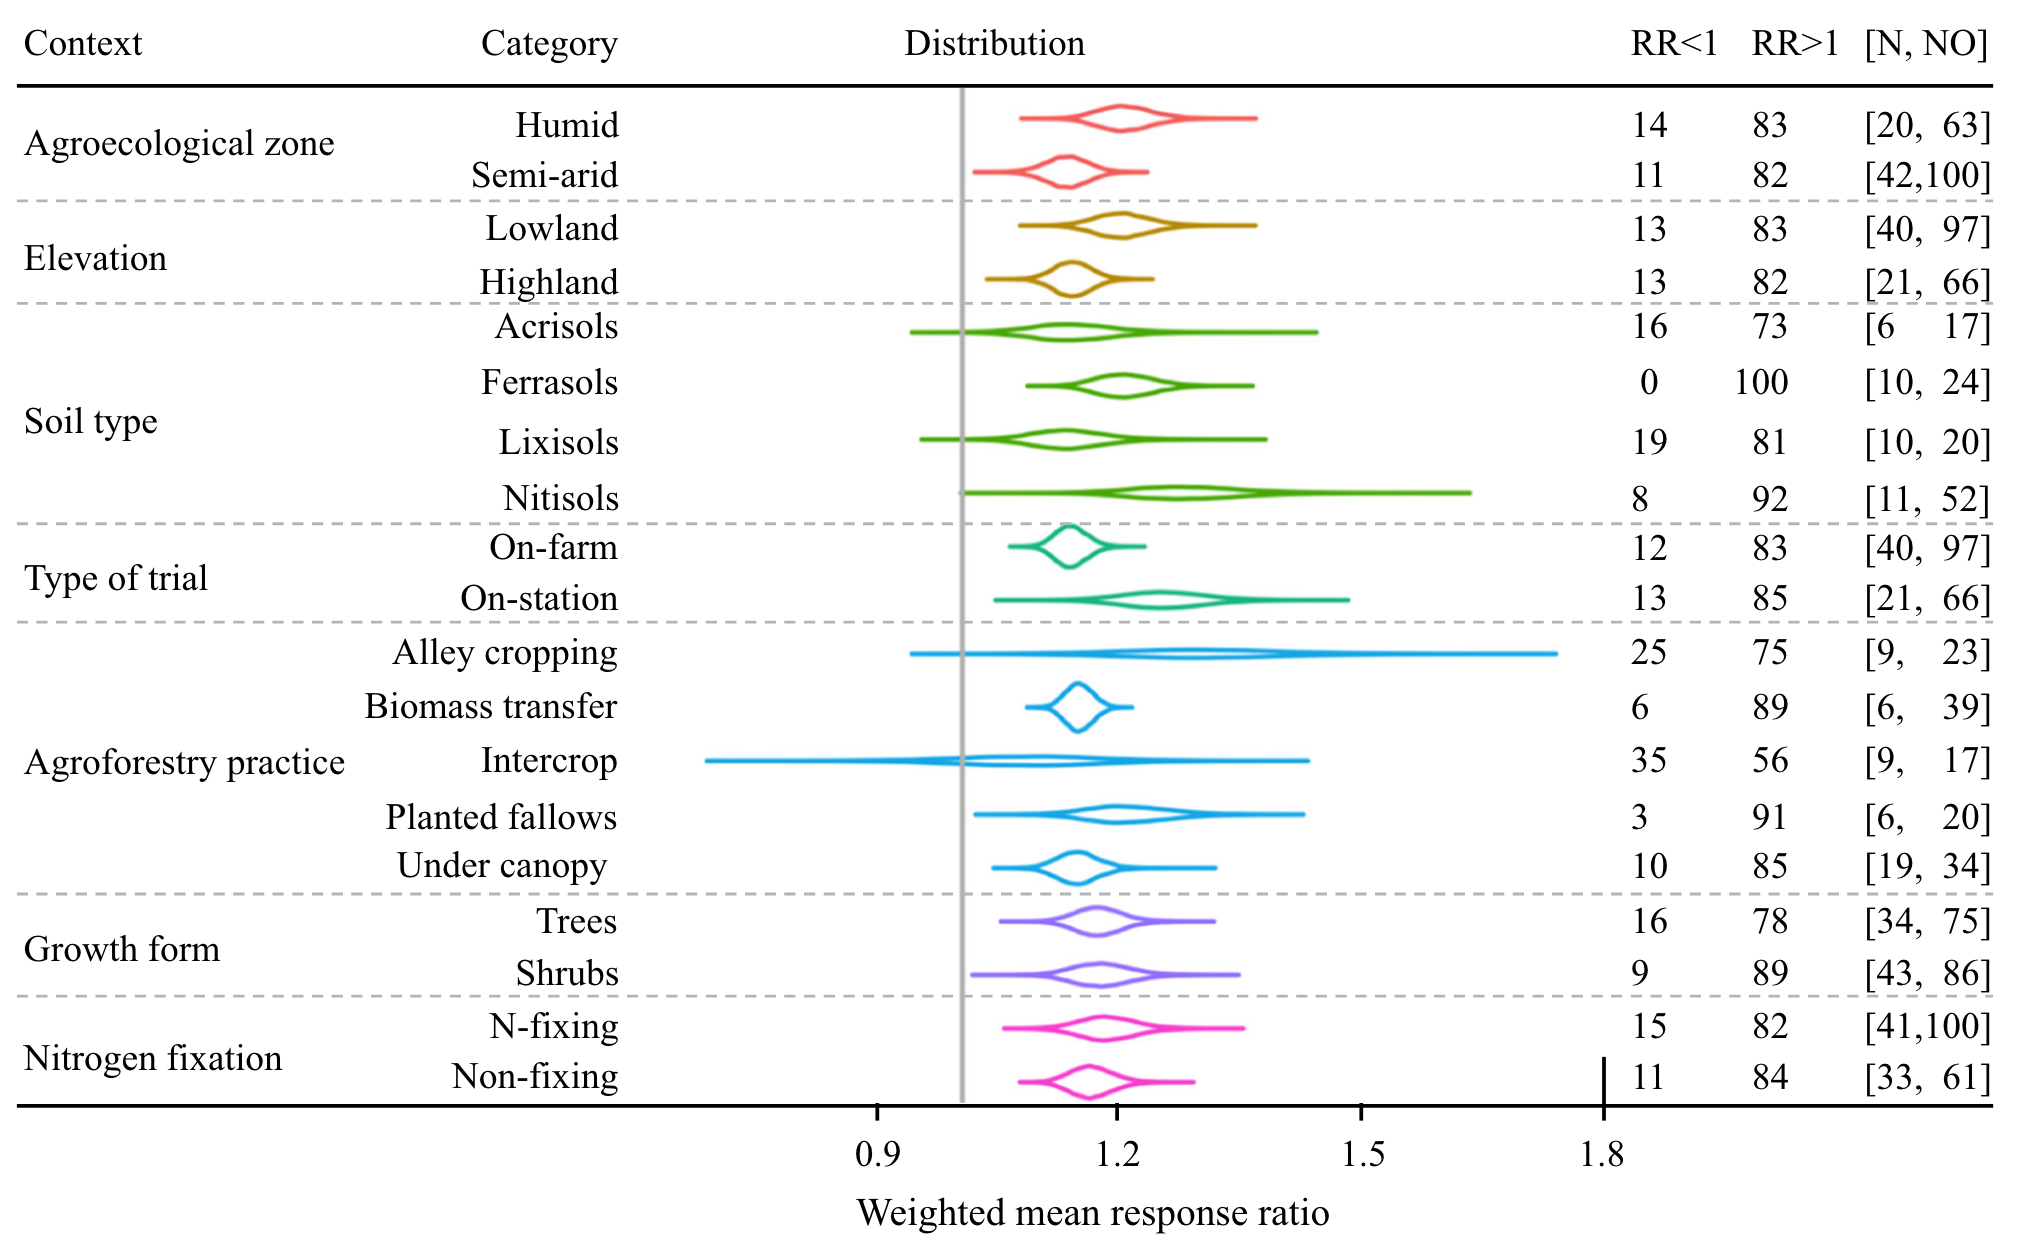
\includegraphics[width=1\linewidth,]{figures/kuyah_agroforestry_violin} 

}

\caption{\label{fig:kuyah_agroforestry_violin}Meta-analysis results of agroforestry effects on nitrogen under varied conditions (Kuyah et al. 2019).}\label{fig:kuyah_agroforestry_violin}
\end{figure}

\end{landscape}

Despite its potential, the widespread adoption and optimization of
agroforestry remain constrained by the complexity of these systems and
uncertainties surrounding long-term outcomes. Decision-makers, farmers,
and policymakers often struggle to assess the risks and benefits of
agroforestry interventions, given the delayed returns and variability in
performance across different landscapes. To address these challenges,
decision-support tools that integrate probabilistic modeling are
essential. In Do \emph{et al.} (2020), we applied decision analysis to
model agroforestry interventions aimed at improving livelihoods in
Vietnam's northern highlands. Figure \ref{fig:do_method_agrof_2020}
outlines the four stages of decision analysis applied to the case study
on agroforestry in Vietnam.

\begin{figure}[H]

{\centering 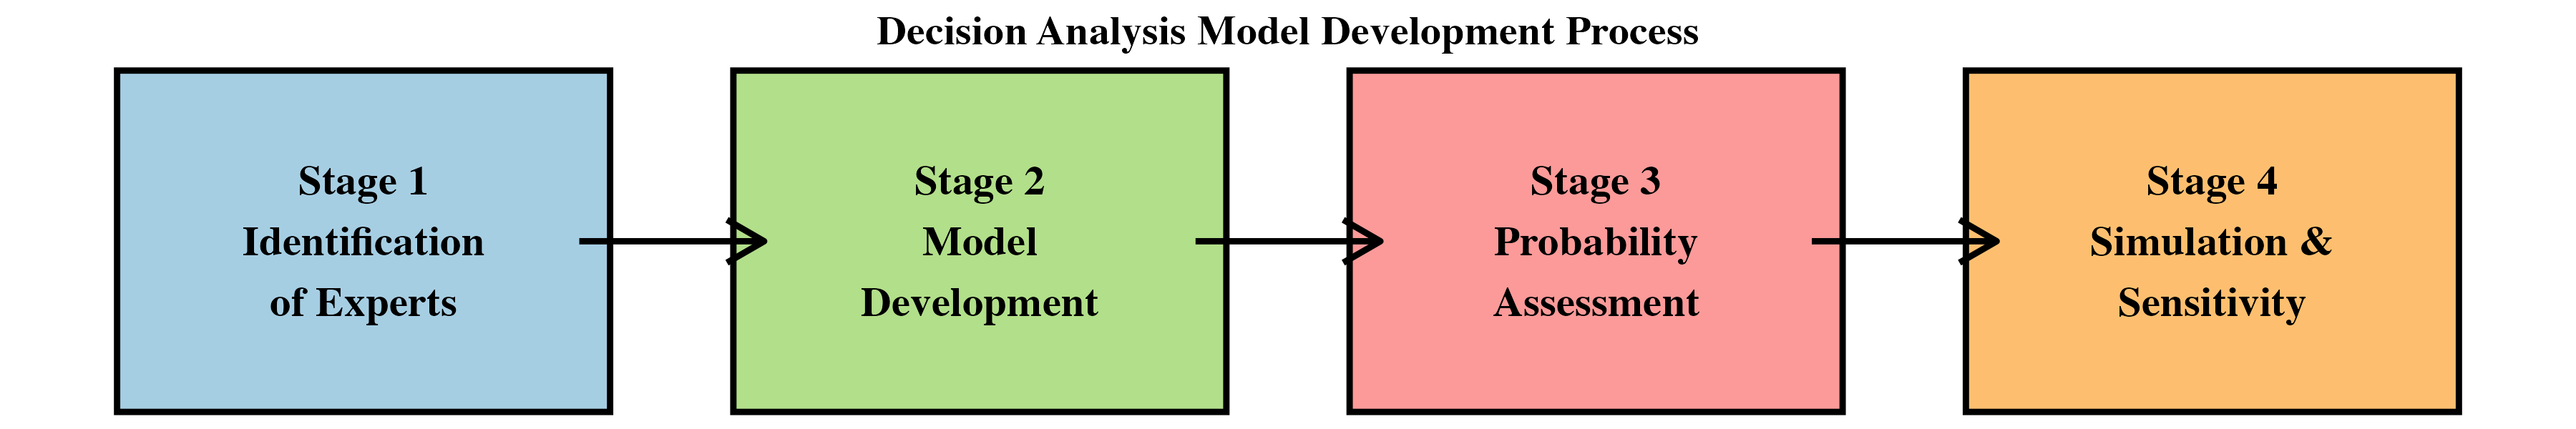
\includegraphics[width=1\linewidth,]{figures/do_method_agrof_2020} 

}

\caption{\label{fig:do_method_agrof_2020}Outline of four stages of decision analysis applied to a case study on agroforestry in Vietnam (Do et al. 2020).}\label{fig:do_method_agrof_2020}
\end{figure}

Farmers' preferences for annual monocultures, driven by immediate
financial returns, present a major barrier to agroforestry adoption. Our
agroforestry models in Vietnam revealed that while monocultures offer
short-term profits, they contribute to long-term soil degradation and
declining yields. In contrast, agroforestry systems provide substantial
long-term benefits, including improved soil fertility and greater
resilience to climatic variability. However, their adoption is
constrained by high establishment costs, delayed financial returns, and
uncertainties in yield stability and market access. These challenges
underscore the importance of decision-support tools that can model
uncertain outcomes and guide effective policy interventions.

One promising strategy for overcoming these adoption barriers is fruit
tree--based agroforestry, which has been promoted in upland Northwest
Vietnam as an alternative to staple crop monocultures. While much
research has focused on plot-level agroforestry performance, there is
limited understanding of how farmers perceive and manage these systems
at the whole-farm scale. In Do \emph{et al.} (2024), we examined the
decision-making processes of agroforestry farmers, identifying key
barriers to widespread adoption and the strategies farmers use to
navigate management challenges. By integrating farmer perspectives with
decision analysis, we highlighted the importance of targeted
interventions that align with farmers' risk perceptions and economic
constraints.

Our models captured trade-offs between short- and long-term returns,
identifying uncertainties such as time preferences and crop prices. We
applied probabilistic methods to assess agroforestry adoption risks,
providing smallholder farmers with actionable insights to navigate
uncertainties and optimize land-use strategies (Fig.
\ref{fig:do_af_model}). Our work integrated probabilistic decision
modeling to assess the long-term performance of agroforestry
interventions under uncertainty. By simulating multiple agroforestry
scenarios, we identified key factors influencing adoption decisions,
including financial risks, labor demands, and expected long-term
benefits. Our results showed that maize-based agroforestry systems,
despite requiring higher initial investments, offered the most resilient
and economically viable option for smallholder farmers, while
coffee-based systems showed potential for diversification but carried
greater uncertainty in returns. This decision-support approach enabled
us to quantify trade-offs between short-term risks and long-term
benefits, providing actionable insights for policymakers and farmers
navigating agroforestry adoption in complex, uncertain environments.

\begin{landscape}

\begin{figure}[H]

{\centering 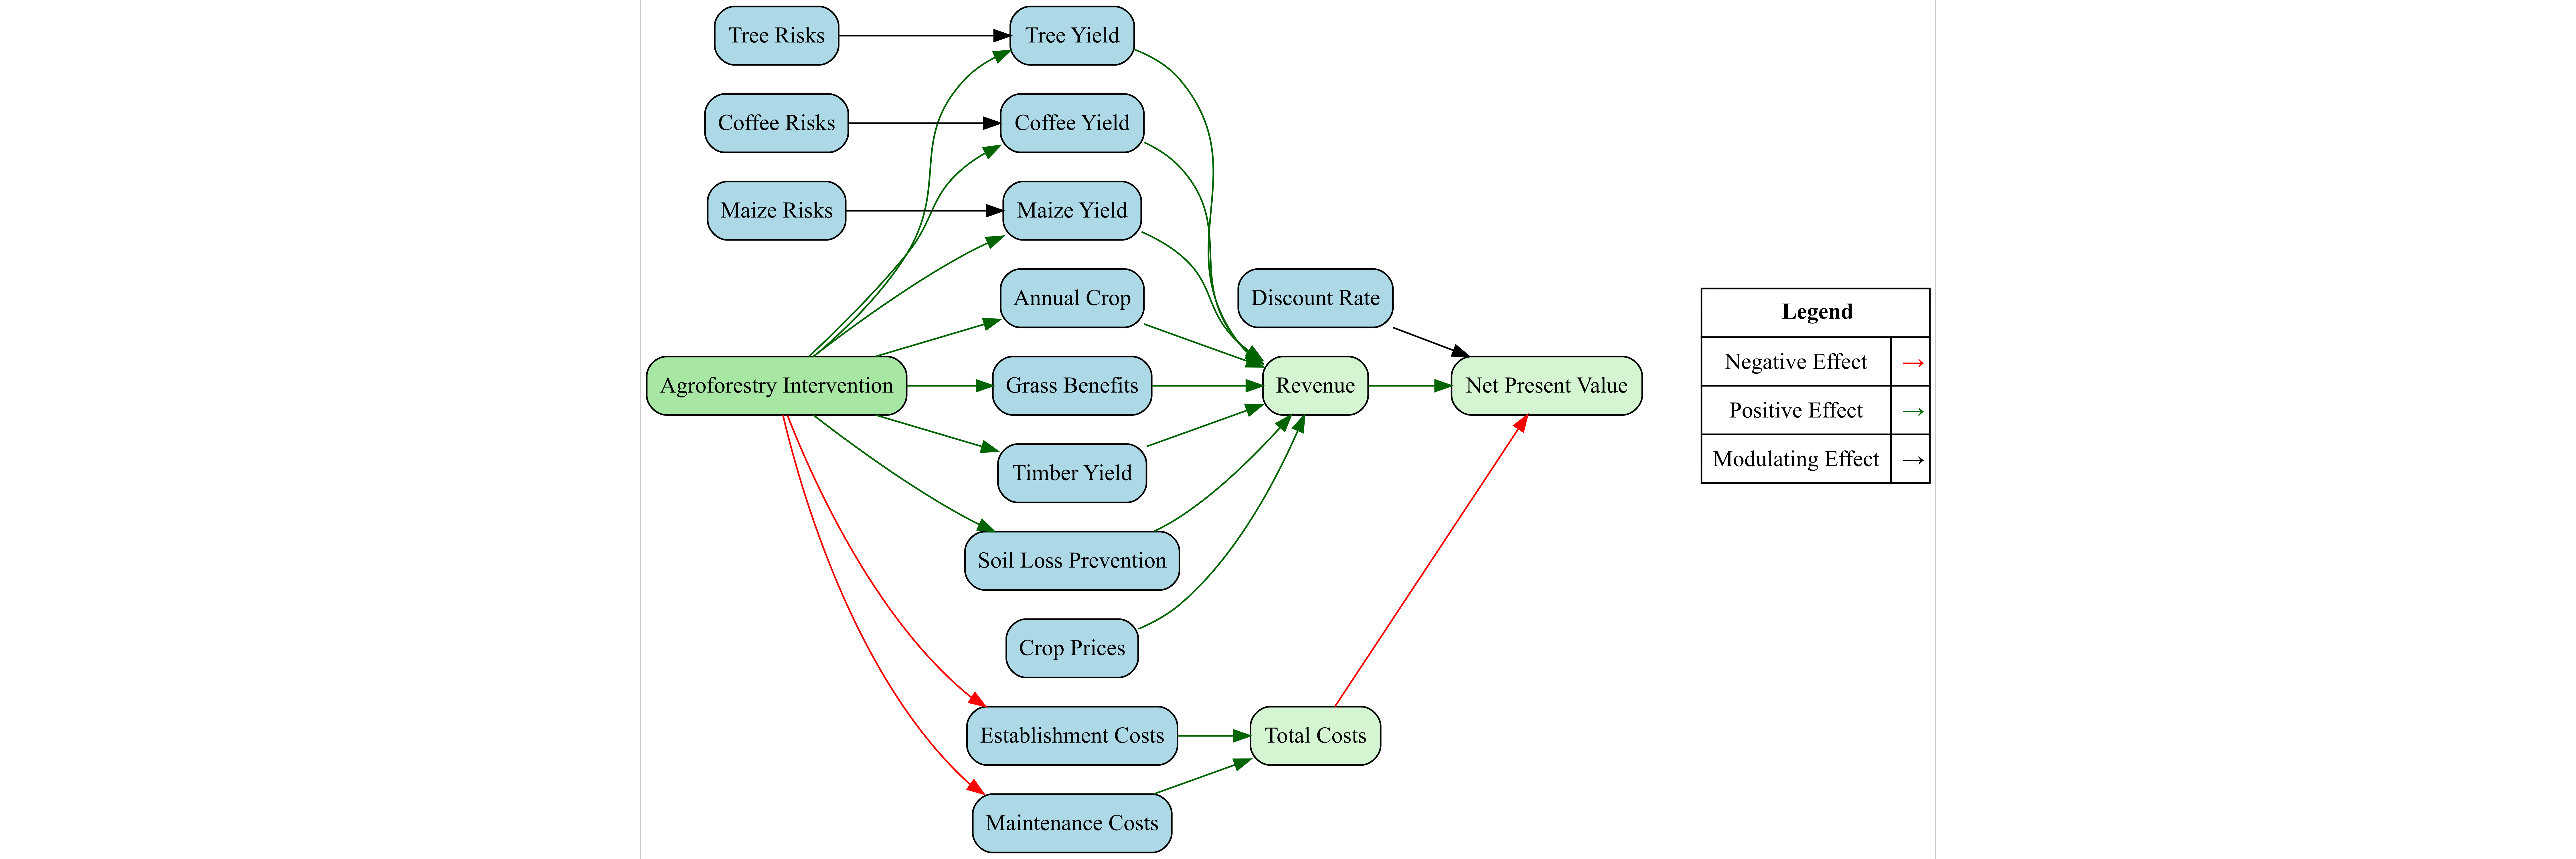
\includegraphics[width=1\linewidth,]{figures/do_af_model} 

}

\caption{\label{fig:do_af_model}Conceptual cost-benefit analysis for agroforestry in Northwest Vietnam. “Tree yield” indicates Shan tea harvest, son tra fruits, longan fruits, mango fruits, plum fruits, and macadamia nuts (Do et al. 2020).}\label{fig:do_af_model}
\end{figure}

Figure \ref{fig:do_af_model} illustrates the conceptual cost-benefit analysis framework applied to agroforestry systems in Northwest Vietnam. It visually represents the trade-offs between different agroforestry strategies, highlighting the role of yield variability, investment costs, and long-term financial returns. By incorporating expert-elicited probabilities and Monte Carlo simulations, the model accounts for uncertainties in crop yields, labor demands, and market fluctuations. This visualization supports our probabilistic assessment by clarifying the relative economic viability of different agroforestry configurations, helping stakeholders evaluate the risks and benefits of various land-use decisions.
\end{landscape}

Beyond Vietnam, agroforestry is increasingly recognized as a sustainable
alternative to monocultures in development contexts, offering solutions
to food insecurity, soil degradation, and climate adaptation. However,
the success of agroforestry depends on a nuanced understanding of
tree-crop-environment interactions and their context-specific
implications for ecosystem service provision. Woody perennials support
billions of people worldwide, yet their establishment, management, and
use vary significantly across regions. In Tabuti \emph{et al.} (2022),
we examined the diversity, uses, and cultural significance of woody
species in agroforestry, identifying the values that drive farmers and
communities to maintain and protect these plants. This research
highlights the need for locally adapted agroforestry strategies that
align ecological benefits with social and economic priorities.

Voluntary standards play a critical role in ensuring the integrity of
carbon offset projects, including those in agroforestry, by regulating
the sale of carbon certificates. However, managers of these projects
face significant uncertainties regarding the costs, risks, and financial
viability of certification. In Netter \emph{et al.} (2022), we applied
Decision Analysis to evaluate the investment potential of carbon
certificates in agroforestry, using Monte Carlo simulations to forecast
financial outcomes under different marketing strategies. Our findings
revealed that while certification can enhance long-term returns, the
financial feasibility of carbon offset agroforestry projects depends on
market conditions, pricing strategies, and risk tolerance (Fig.
\ref{fig:netter_cashflow}).

Figure \ref{fig:netter_cashflow} shows the results of an ex-ante
analysis of the decision to certify an agroforestry site in Costa Rica
with a voluntary carbon offset label, with three marketing strategies:
(1) Sale of carbon-neutral products, (2) Direct sale of Verified
Emission Reductions (VER), (3) Pass VER on to company shareholders.
Plots show the projected probability distributions of the annual cash
flows

\begin{figure}[H]

{\centering 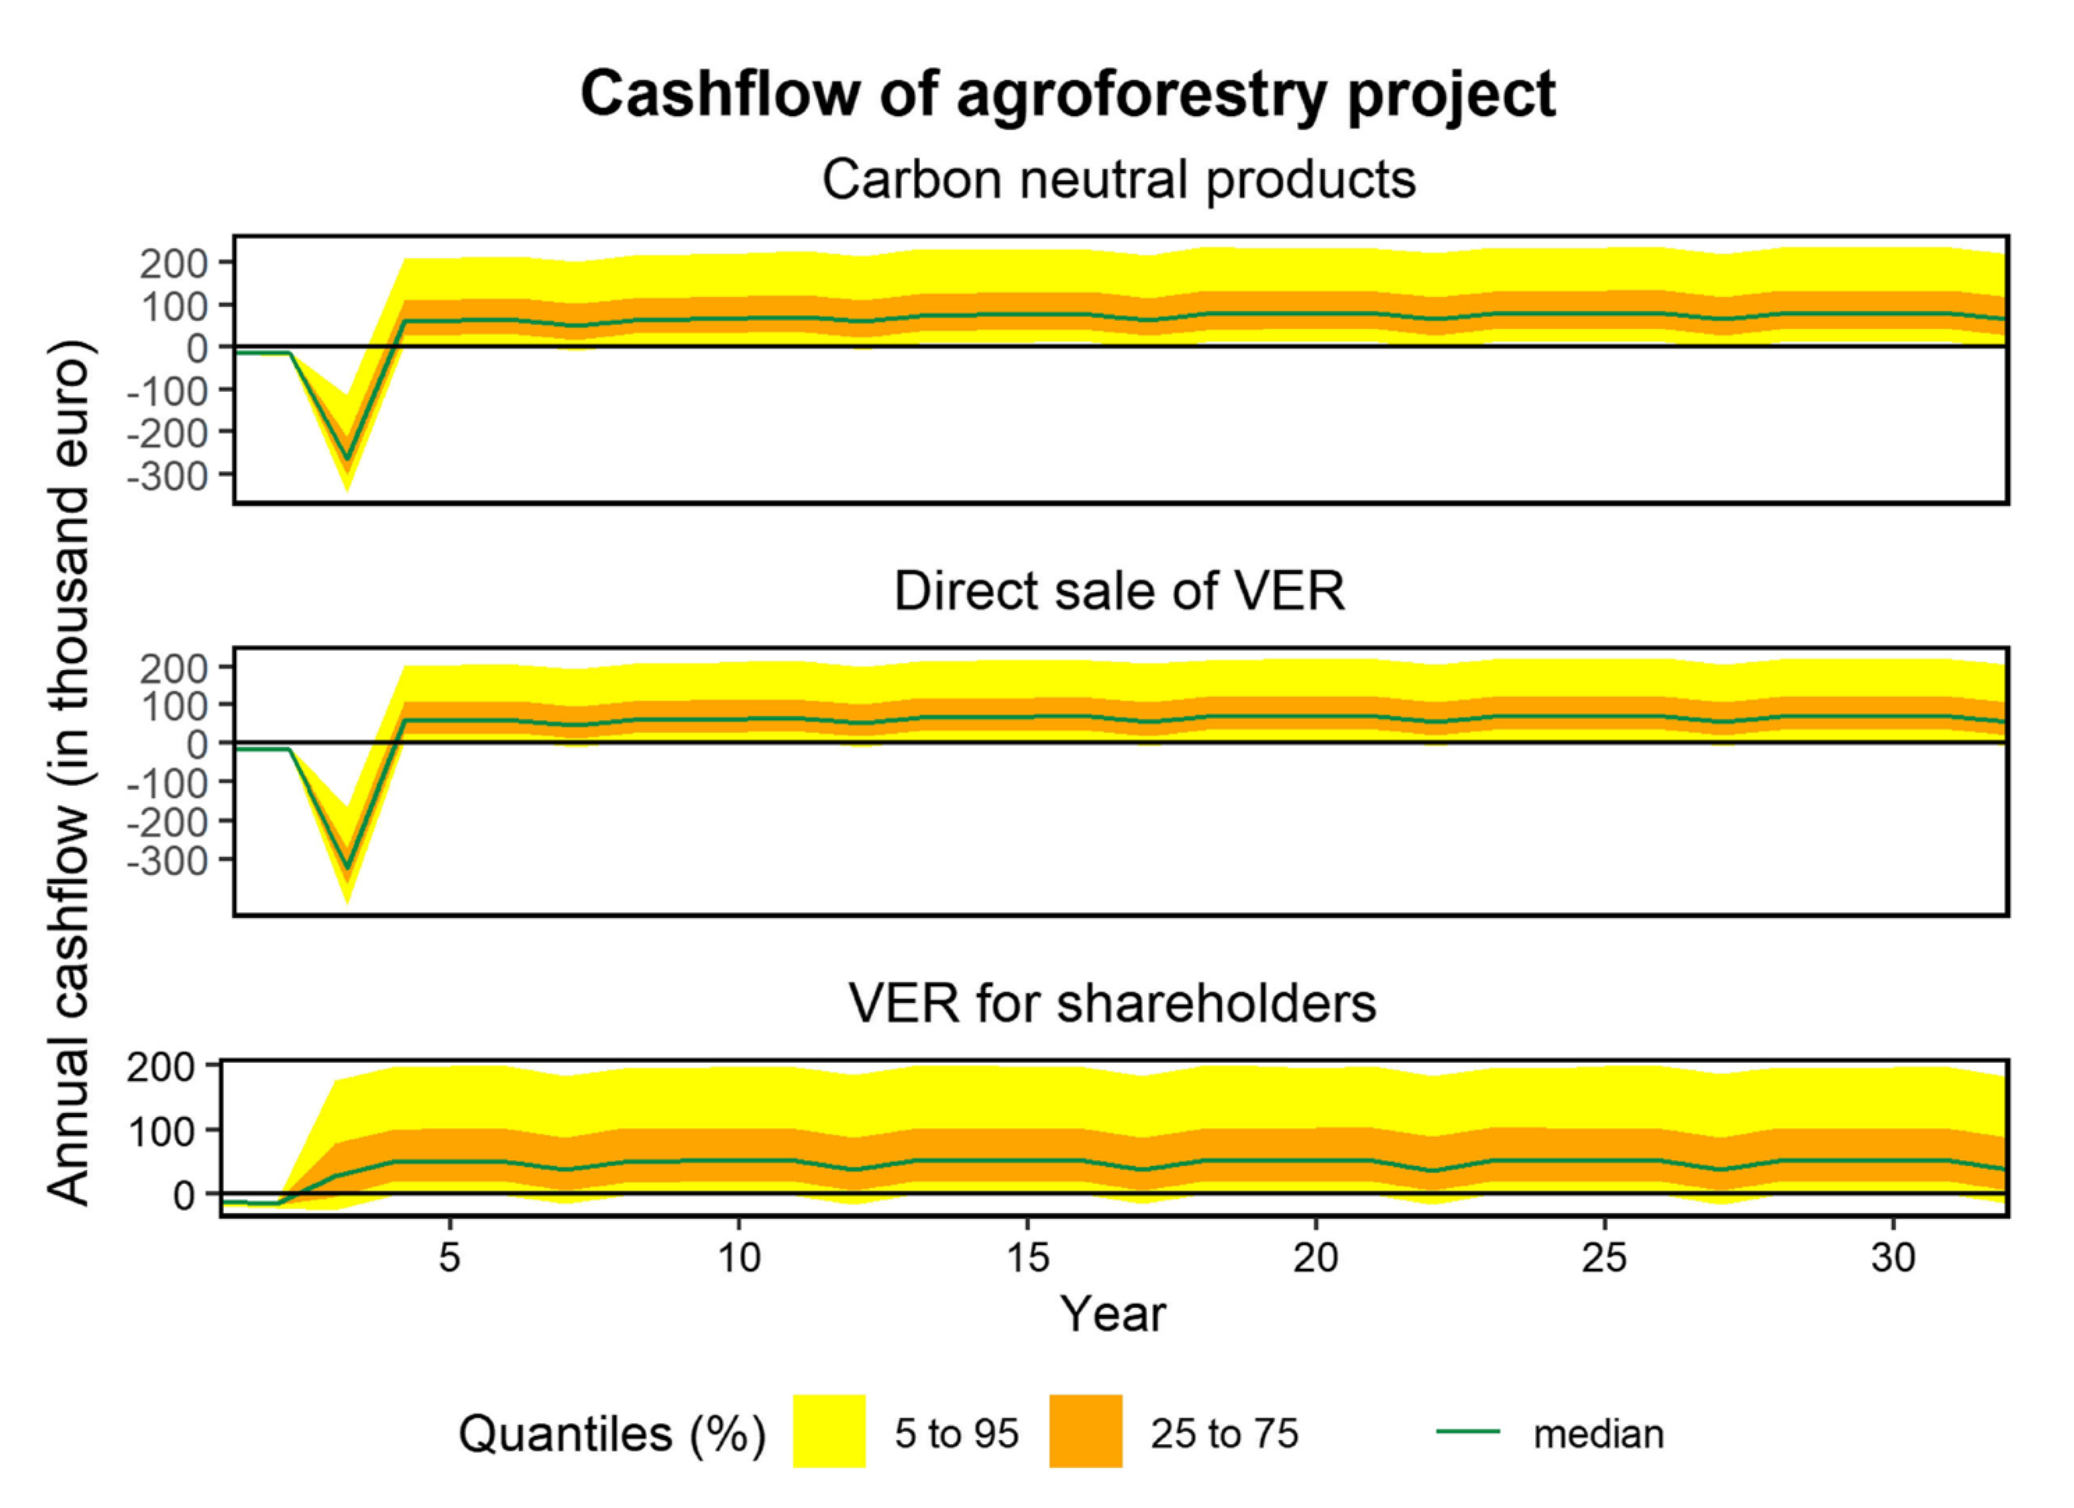
\includegraphics[width=0.8\linewidth,]{figures/netter_cashflow} 

}

\caption{\label{fig:netter_cashflow}Cash flow outputs of a Monte Carlo simulation (with 10,000 model runs) (Netter et al. 2022)}\label{fig:netter_cashflow}
\end{figure}

More broadly, probabilistic modeling provides a powerful framework for
navigating the uncertainties inherent in agroforestry systems. By
integrating expert knowledge, empirical data, and scenario analysis,
these models enable ex-ante assessments of agroforestry interventions,
highlighting key uncertainties and trade-offs that influence adoption
decisions. Our research demonstrates how decision-support tools can
reduce knowledge gaps, provide plausible outcome ranges, and enhance the
design of targeted, risk-aware interventions.

Beyond individual projects, my work in agroforestry research bridges
scientific insights with actionable policy, ensuring that interventions
are both ecologically sound and economically viable. By applying
probabilistic models to agroforestry decision-making, we have developed
tools that empower farmers, policymakers, and development practitioners
to make informed choices. These contributions illustrate how integrating
agroforestry with advanced decision-support approaches can provide a
scalable, sustainable pathway for agricultural transformation---one that
balances human well-being with ecological resilience.

\hypertarget{assessing-management-strategies-in-horticulture}{%
\subsection{Assessing Management Strategies in
Horticulture}\label{assessing-management-strategies-in-horticulture}}

Horticultural production faces numerous uncertainties, from climate
variability and pest pressures to market fluctuations and resource
constraints. Effective decision-making in this sector requires tools
that can account for these complexities and provide robust, scientific
insights. Probabilistic decision models offer a powerful approach to
quantify risks, assess trade-offs, and optimize management strategies.
My research applies Bayesian networks, Monte Carlo simulations, and
expert-driven modeling to support horticultural decision-making,
enabling growers, researchers, and policymakers to navigate uncertainty
and design more resilient and sustainable horticultural systems.

Advancing horticultural production requires data-driven decision-support
tools that can account for variability in crop performance, resource
availability, and environmental conditions. In my research, I have
applied probabilistic modeling, hyperspectral imaging, and model-based
assessments to optimize horticultural management, integrating
uncertainty analysis and precision agriculture techniques to improve
outcomes.

Hyperspectral imaging has emerged as a powerful tool for monitoring
plant health, detecting stress factors, and optimizing resource use in
horticultural systems. In Ruett \emph{et al.} (2022a) and Ruett \emph{et
al.} (2022b), we applied high-resolution spectral data and model-based
assessments to quantify plant traits and assess crop performance. These
studies demonstrated how remote sensing combined with decision modeling
can provide real-time, non-destructive monitoring of horticultural
crops, improving early detection of nutrient deficiencies and disease
stress.

Beyond monitoring, probabilistic decision models offer a structured
approach to optimizing horticultural management under uncertainty. In
Ruett \emph{et al.} (2020), we developed stochastic models to simulate
resource allocation, yield variability, and economic trade-offs, helping
to guide strategic decision-making.

Crop models can support agricultural decisions, yet their reliability is
necessarily limited when they do not sufficiently represent the
complexity and specific circumstances of the target system. In some
cases, models have such prohibitively high data requirements that they
are only applicable with far-reaching and often questionable
assumptions. In Liman Harou \emph{et al.} (2021), we demonstrate a
customizable solution-oriented approach for crop modelling in situations
where data and resources are limited (Fig.
\ref{fig:liman_protocol_bayes}).

\begin{figure}[H]

{\centering 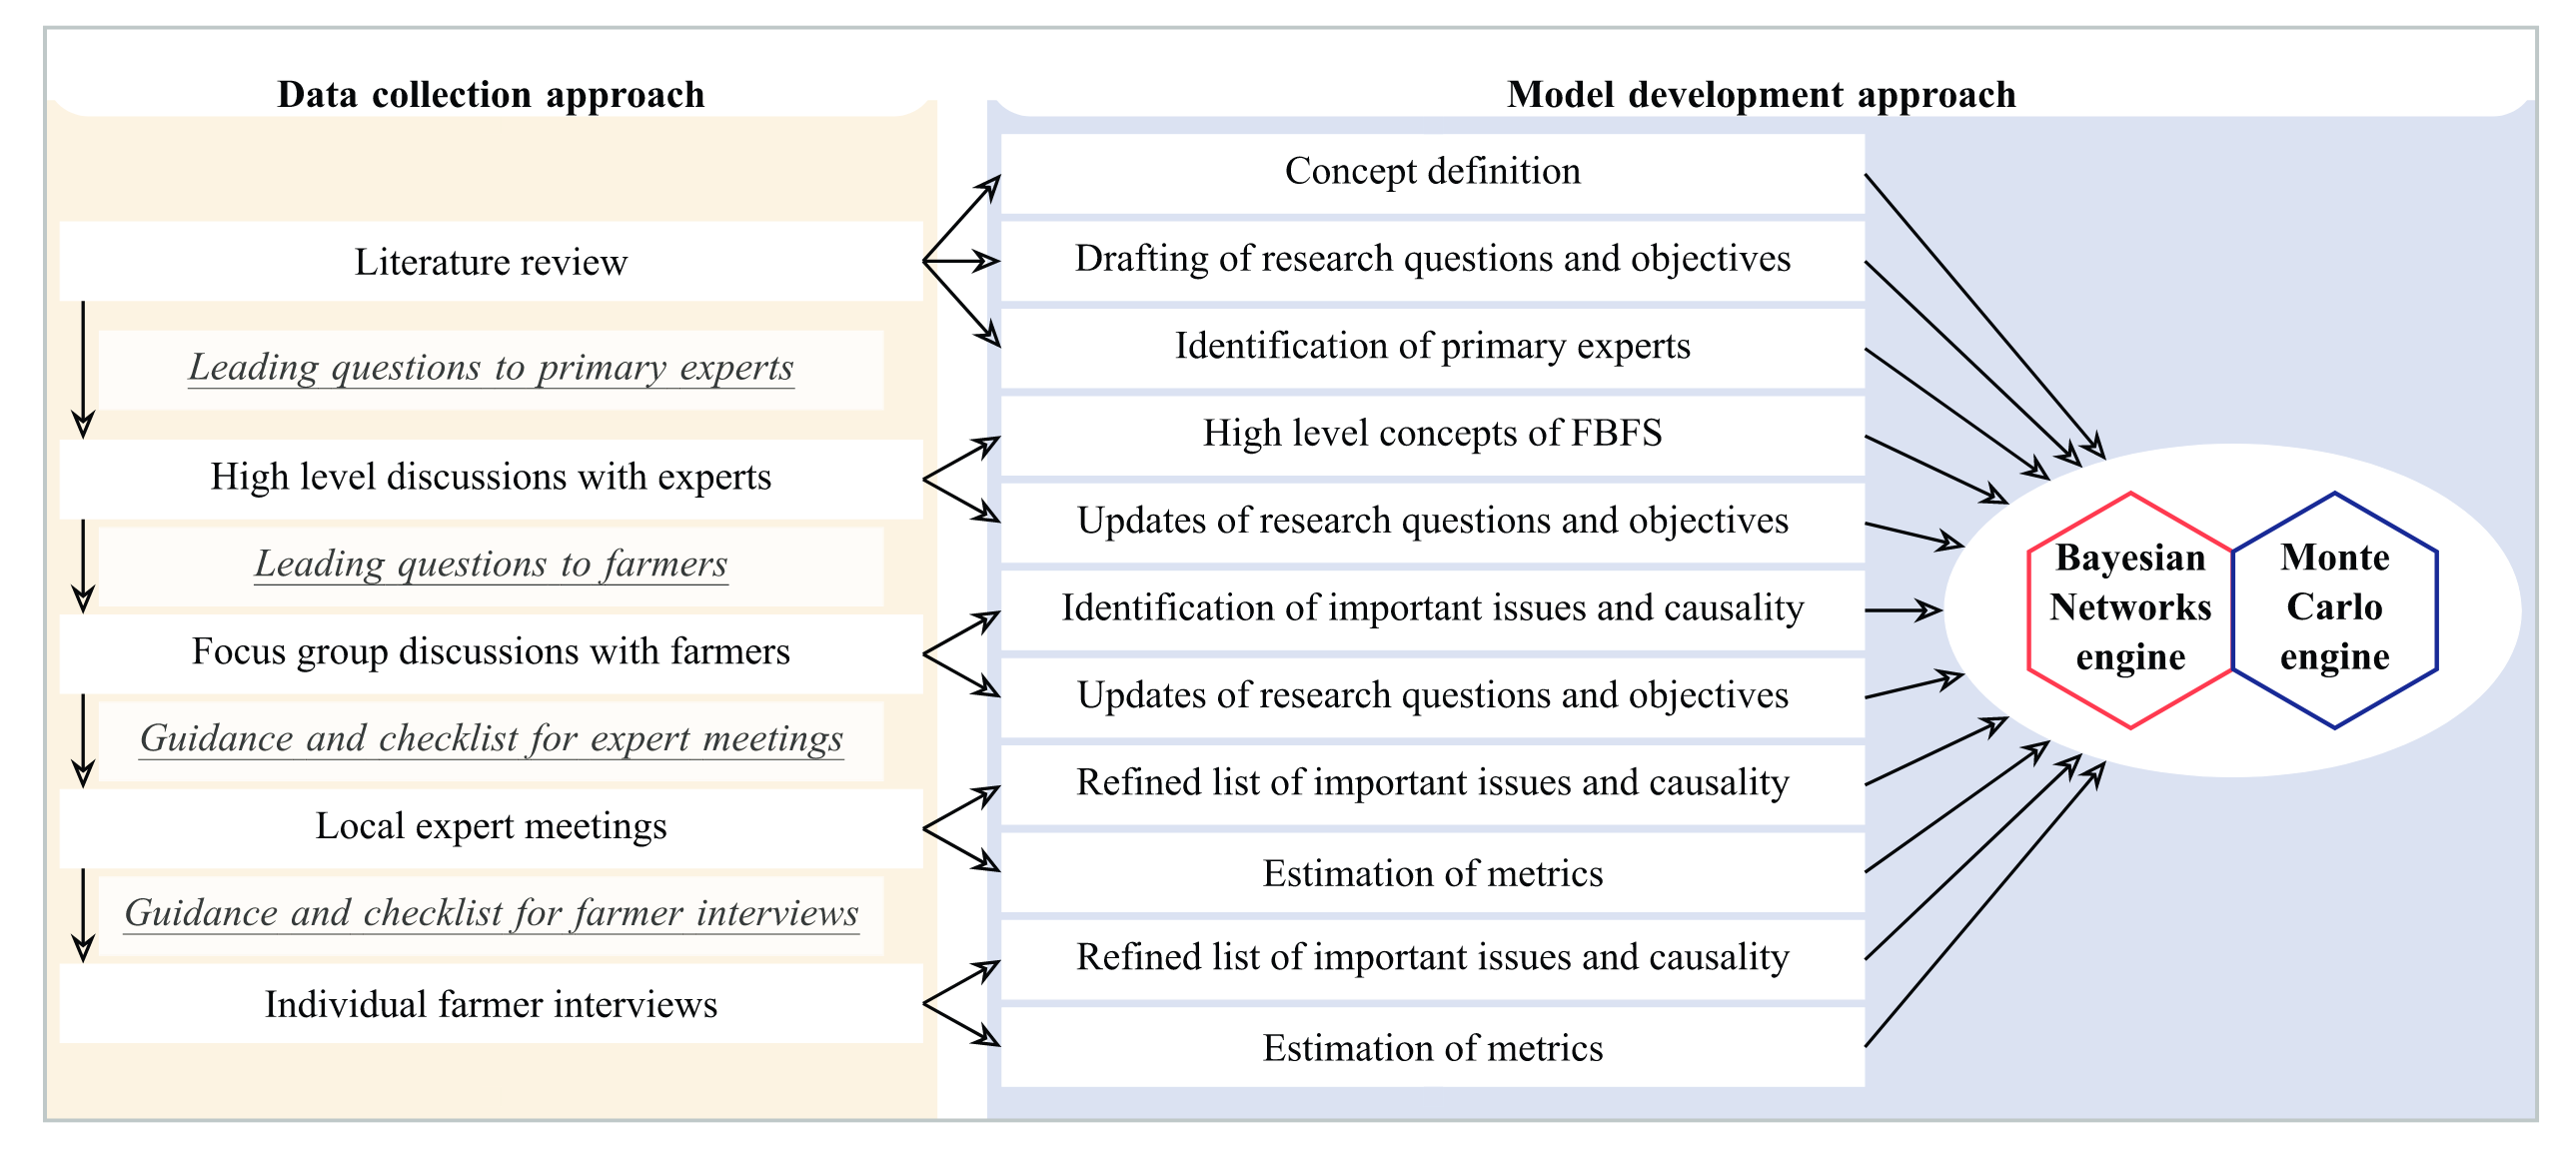
\includegraphics[width=0.8\linewidth,]{figures/liman_protocol_bayes} 

}

\caption{\label{fig:liman_protocol_bayes}Approach for developing a crop model for flood-based farming systems in Ethiopia and Kenya (Liman et al. 2021).}\label{fig:liman_protocol_bayes}
\end{figure}

A broader holistic decision-analysis framework is essential for
addressing the complex, multi-dimensional challenges in horticultural
and agricultural systems. In Kamau \emph{et al.} (2021), we applied
multi-criteria decision analysis and expert-driven probabilistic models
to assess farm sustainability across ecological, economic, and social
dimensions. Our findings highlight the need for improved sustainability
planning and reporting, particularly in farm management practices and
farmer support systems. The study revealed no significant differences in
overall sustainability performance between farm types, but certified
organic farms demonstrated higher economic resilience and environmental
integrity due to better training and support. Additionally, regional
factors played a crucial role, with farms in Murang'a exhibiting
stronger sustainability indicators than those in Kajiado, largely due to
differences in land tenure security, conflict resolution mechanisms, and
resource conservation strategies. The sustainability performance
assessment (Fig. \ref{fig:Kamau_2021}) underscores the value of
structured decision frameworks in guiding policy and farm-level
interventions to enhance long-term resilience in smallholder
agriculture.

\begin{figure}[H]

{\centering 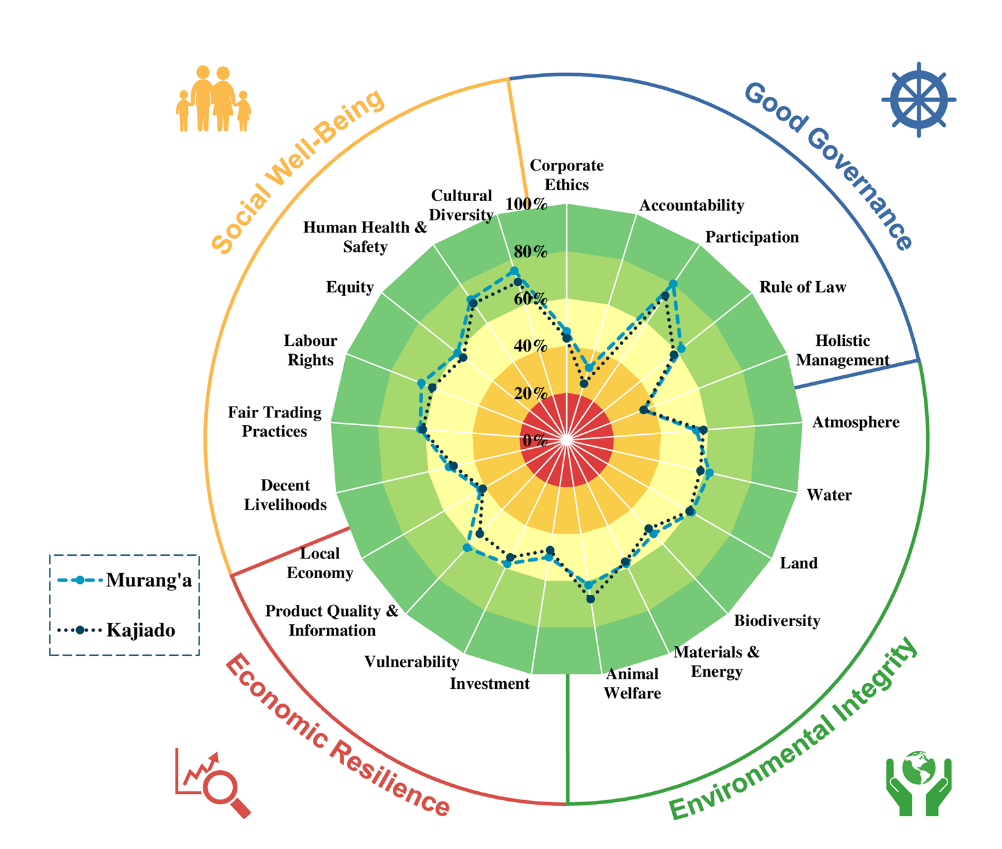
\includegraphics[width=0.8\linewidth,]{figures/Kamau_2021} 

}

\caption{\label{fig:Kamau_2021}Overall performance in degree of goal achievement (DGA) from the SMART-Farm Tool across four sustainability dimensions and 21 sustainability themes for 400 farms in Kajiado and Murang’a counties in Kenya (Kamau et al. 2021).}\label{fig:Kamau_2021}
\end{figure}

These innovations illustrate how probabilistic modeling, remote sensing,
and decision analysis can enhance horticultural sustainability, enabling
more precise, data-driven, and resilient agricultural practices. My work
in this area demonstrates how advanced decision-support tools can bridge
the gap between scientific insight and practical implementation,
equipping growers, policymakers, and researchers with strategic,
evidence-based approaches for sustainable horticultural production.

\hypertarget{informing-water-resources-management}{%
\subsection{Informing Water Resources
Management}\label{informing-water-resources-management}}

Water availability and hydrological variability play a crucial role in
shaping agricultural systems, particularly in regions where seasonal
flooding and fluctuating water resources influence farming decisions.
Managing these uncertainties requires probabilistic models, remote
sensing techniques, and decision-support tools to inform sustainable
water use strategies. My research applies stochastic modeling,
hydrological analysis, and spatial mapping to improve water resource
management, with a focus on flood-based farming systems, water
allocation trade-offs, and hydrological forecasting.

In Whitney \emph{et al.} (2025), we developed a probabilistic framework
for evaluating the trade-offs between agricultural water use and
conservation priorities. This model accounts for uncertainties in water
availability, demonstrating how decision-support tools can optimize
irrigation strategies while balancing environmental and productivity
goals. By integrating stochastic hydrological simulations, this approach
helps decision-makers navigate competing demands for water resources in
agriculture.

\begin{landscape}

\begin{figure}[H]

{\centering 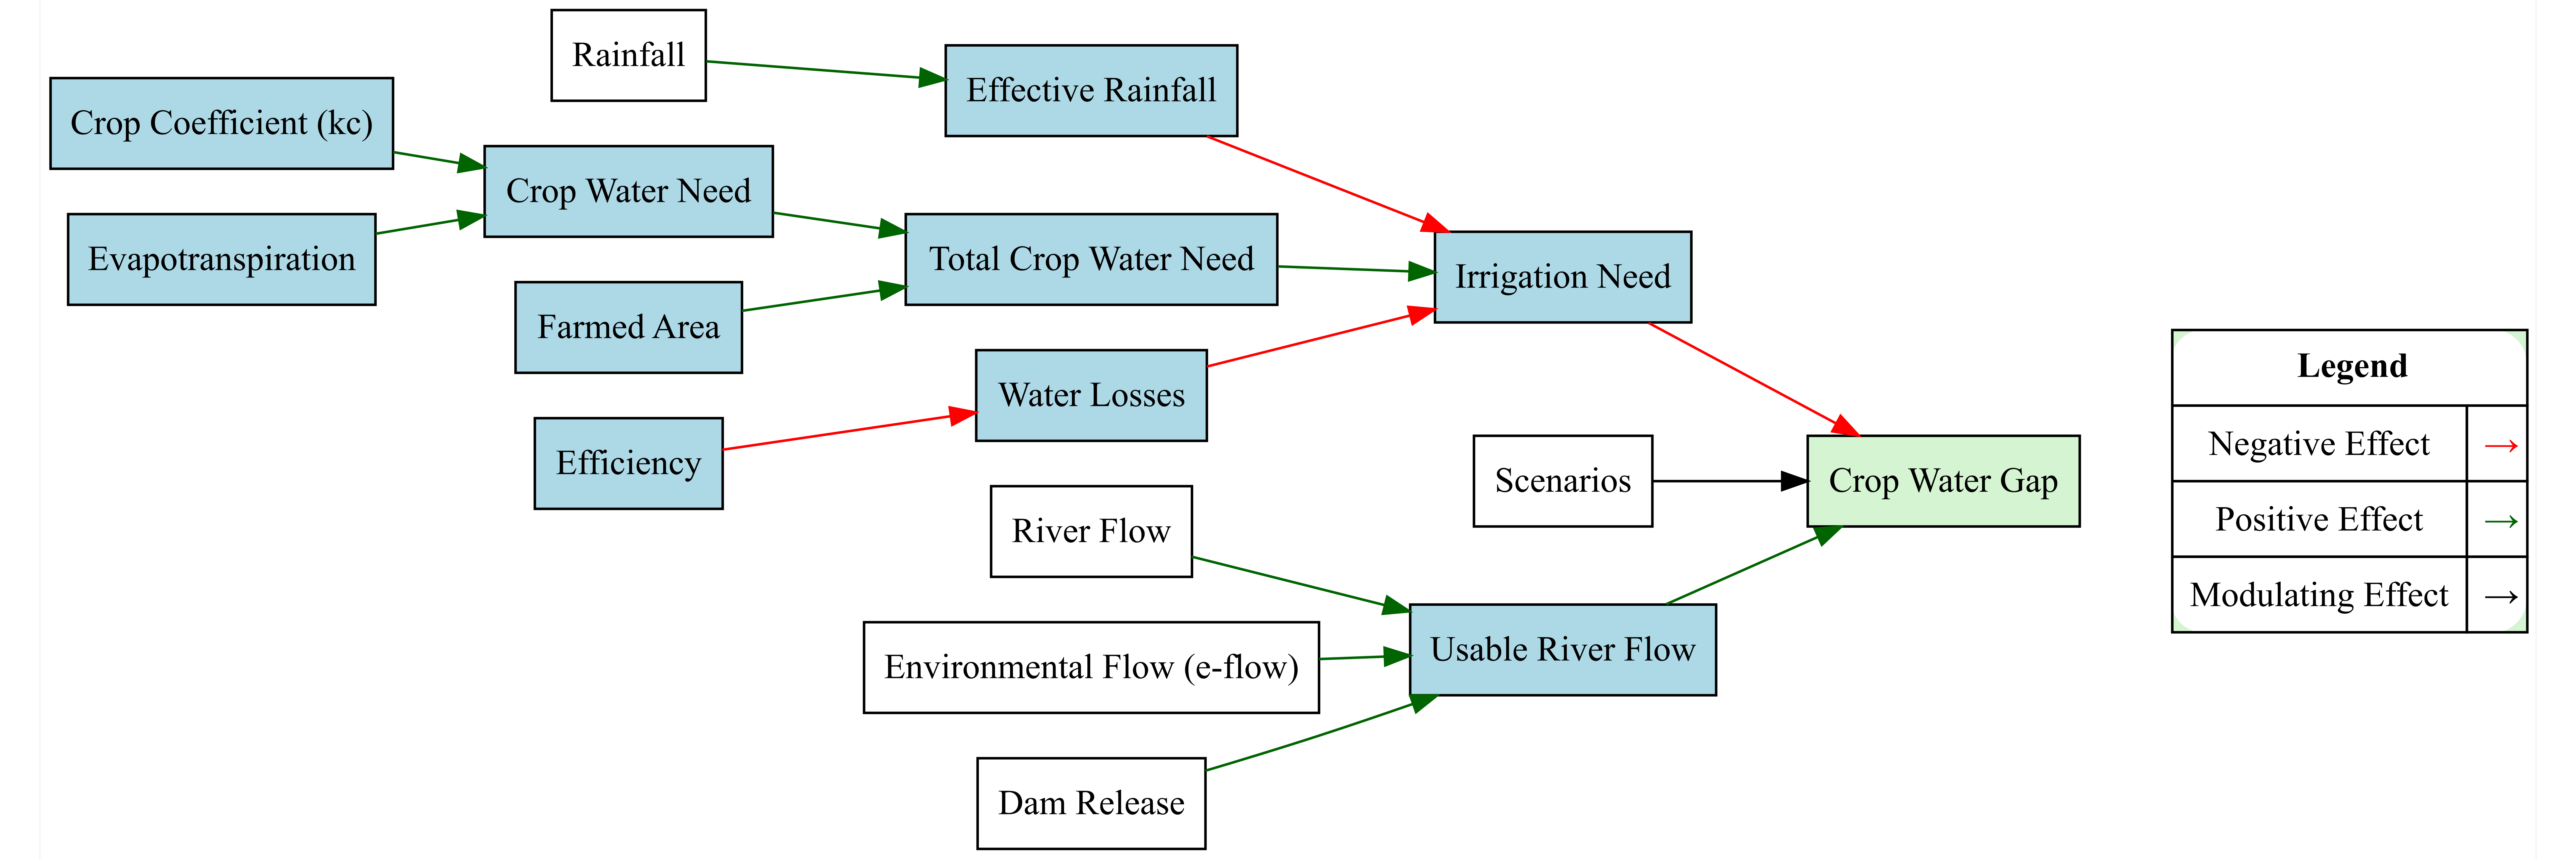
\includegraphics[width=1\linewidth,]{figures/limpopo_model} 

}

\caption{\label{fig:limpopo_model}Conceptual model illustrating the key components and relationships driving water needs for agriculture and environmental flow (e-flow) management in the Letaba River Basin (Whitney et al. 2025).}\label{fig:limpopo_model}
\end{figure}

Figure \ref{fig:limpopo_model} illustrates the key components and interactions influencing water needs in the Letaba River Basin, highlighting the relationships between rainfall, river flow, irrigation demand, and environmental flow (e-flow) management. The model provides a structured approach for assessing the socioecological impacts of e-flow policies on smallholder farming. Our findings indicate that while the irrigation water demand of small-scale agriculture is significantly lower than the required e-flow volume, farmers experience substantial crop water gaps, particularly during dry seasons. These deficits threaten agricultural sustainability and may require upstream water flow supplementation, though this would necessitate restricting current upstream usage. The decision-support framework integrates expert knowledge and Monte Carlo simulations to evaluate e-flow management options under uncertainty. By extending the e-flow concept to include the needs of smallholder farmers, the model equips decision-makers with a robust tool for balancing ecological conservation with agricultural water security, even in data-limited contexts.

\end{landscape}

Spatial uncertainty in flood-based farming systems and land-use planning
presents another challenge that deterministic models struggle to
address. Traditional remote sensing approaches often misclassify
agricultural landscapes due to spectral similarity and system
variability. By integrating Bayesian networks with expert-driven
probability models, we have developed probabilistic mapping approaches
that improve classification and decision-making in dynamic landscapes
(Liman Harou \emph{et al.} 2020).

In Liman Harou \emph{et al.} (2020), we applied spatial analysis
techniques to map and classify flood-based farming systems, addressing
challenges in distinguishing cropping practices influenced by
hydrological fluctuations. The study demonstrated that stochastic system
behavior and spectral similarities often lead to misclassification in
traditional remote sensing approaches. By incorporating advanced
classification algorithms and decision-analysis tools, we improved the
accuracy of mapping agricultural water use patterns, providing critical
insights for land-use planning and flood-adaptive farming systems. We
integrated Bayesian networks and remote sensing, enabling probabilistic
mapping of flood-based farming systems in Ethiopia and Kenya (Liman
Harou \emph{et al.} 2020). Together, these studies illustrate how
probabilistic decision models, stochastic hydrological simulations, and
remote sensing techniques contribute to a more data-driven, resilient
approach to water resource management in agriculture. By quantifying
uncertainty and spatial variability, these tools provide a foundation
for evidence-based policy and adaptive water management strategies that
support both agricultural productivity and environmental sustainability
(Fig. \ref{fig:Liman_Mapping_2020}).

Figure \ref{fig:Liman_Mapping_2020} shows the mixed modeling methods we
applied in our work in Kisumu County, Kenya and Tigray region, Ethiopia.
Elliptic shapes mark nonspatial data components described by an
expert-informed Bayesian network. GADM (Global Administrative Areas),
MODIS (Moderate Resolution Imaging Spectroradiometer, SRTM (Shuttle
Radar Topography Mission), hdf (Hierarchical Data Format), GDAL
(Geospatial Data Abstraction Library), and FBFS (flood-based farming
systems) (Liman Harou \emph{et al.} 2020).

\begin{figure}[H]

{\centering 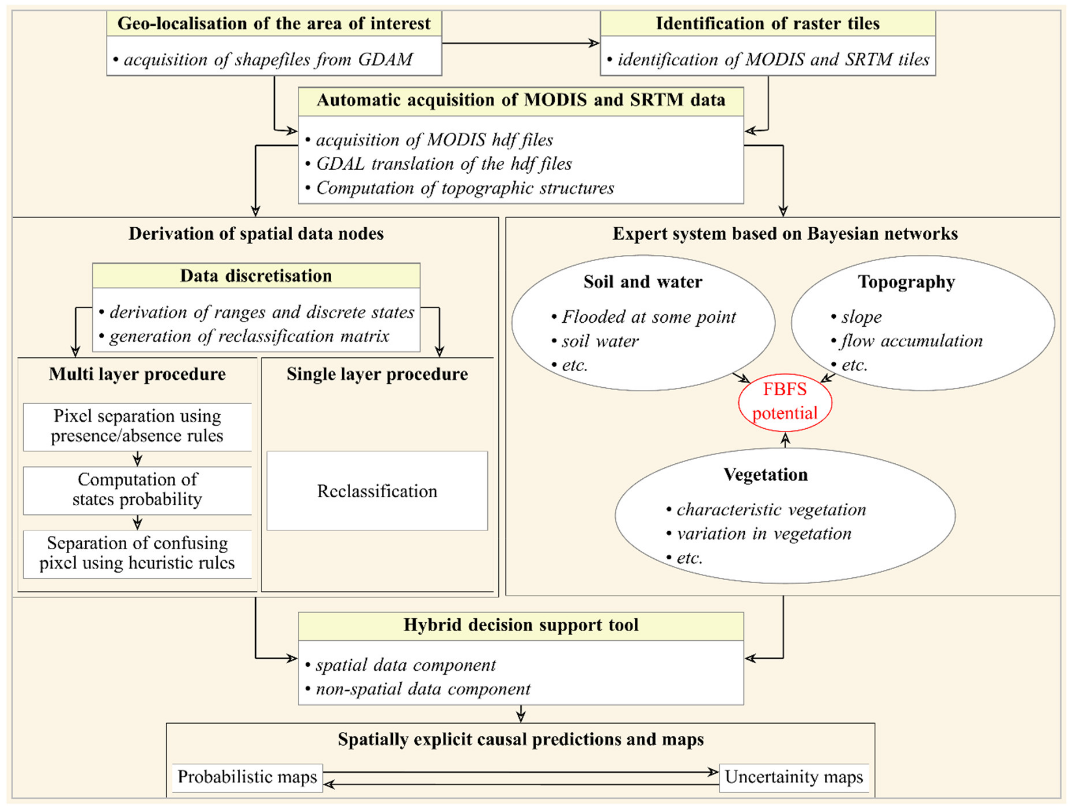
\includegraphics[width=1\linewidth,]{figures/Liman_Mapping_2020} 

}

\caption{\label{fig:Liman_Mapping_2020}Conceptual framework for probabilistic mapping of flood-based farming systems based on expert analysis (Liman et al. 2020)}\label{fig:Liman_Mapping_2020}
\end{figure}

\hypertarget{supporting-climate-adaptation-and-mitigation-interventions}{%
\subsection{Supporting Climate Adaptation and Mitigation
Interventions}\label{supporting-climate-adaptation-and-mitigation-interventions}}

Climate change presents unprecedented challenges to agriculture,
requiring adaptive strategies that enhance resilience while addressing
uncertainties. My research leverages stochastic modeling and decision
analysis to evaluate interventions that support climate adaptation and
risk management at various scales.

In Fernandez \emph{et al.} (2022), we applied decision analysis to
evaluate and prioritize farm management interventions in banana
certification schemes, systematically assessing uncertainties in
production, market risks, and ecological impacts. By structuring
decision pathways with probabilistic models, we quantified the
trade-offs between climate adaptation, mitigation, and economic
viability, helping farmers and policymakers identify the most effective
interventions. The analysis revealed that nutrient management
strategies, such as composting and structured fertilization plans,
provided the highest combined benefits across adaptation, mitigation,
and ecological dimensions. Meanwhile, interventions such as plastic
reduction and land conversion had mixed effects, emphasizing the need
for context-specific decision-making (Fig.
\ref{fig:Fernandez_2022_result}).

Figure \ref{fig:Fernandez_2022_result} shows relative farm-level effects
of interventions. each column of the plot, we show the expected outcomes
from measure implementation, whereas the proposed interventions are
shown in rows. On the y-axis, IPM stands for integrated pest management.
The color in each cell represents the likely effect (estimated as the
median relative effect after 10,000 simulation runs) of the measure on
the expected outcome. In gray, we show no estimated effect, whereas in
blue and red we show positive and negative effects, respectively. The
gray bubble inside each cell (IQR legend) represents the interquartile
range, which is the difference between the third and first quartiles of
the outcome distribution. We used the IQR value to express the
uncertainty of our estimation of effects. Here, lower IQR values
represent greater levels of confidence in the estimate

\begin{figure}[H]

{\centering \includegraphics[width=1\linewidth,]{figures/Fernandez_2022_result} 

}

\caption{\label{Fernandez_2022_result}Relative farm-level effects on climate change adaptation and mitigation, ecology and production costs, change in yield and risks for 21 farm management interventions proposed for sustainable banana production systems in export-oriented banana growing regions of Latin America (Fernandez et al. 2022).}\label{fig:Fernandez_2022_result}
\end{figure}

By integrating expert knowledge with Monte Carlo simulations, the study
provided probability distributions for intervention outcomes, improving
the transparency and robustness of farm certification processes. The
findings underscore the role of decision analysis in guiding sustainable
agricultural transitions, particularly in export-oriented banana
production, where interventions must balance ecological sustainability
with economic feasibility. This structured approach supports informed
decision-making by reducing uncertainty, enabling policymakers and
farmers to adopt resilient and adaptable management strategies.

Rojas \emph{et al.} (2021) further developed modeling approaches by
evaluating investment decisions in Chilean cherry production,
integrating risk and uncertainty into orchard management strategies. We
examined the adoption of orchard covers in sweet cherry production
systems in Chile. By applying decision analysis, we assessed the
economic and ecological trade-offs of this technology under extreme
weather conditions. The findings emphasized the role of targeted
investments in enhancing climate resilience, enabling growers to protect
their crops from variability and reduce financial losses. This study
highlights how innovative management practices can address specific
climate challenges in high-value horticultural systems.

We employed a stochastic impact evaluation framework in Tamba \emph{et
al.} (2021) to simulate returns on investment in forest and landscape
restoration (FLR) in degraded Afromontane forests. By accounting for
uncertainties and risks, our research demonstrated the potential of FLR
interventions to achieve ecological restoration and enhance human
well-being. The use of probabilistic models allowed for a robust
evaluation of long-term outcomes, providing critical insights for
scaling FLR efforts in regions facing environmental degradation.

These studies illustrate the importance of integrating stochastic
modeling and decision analysis into climate adaptation strategies. By
addressing uncertainties and quantifying trade-offs, my research
provides a foundation for designing interventions that enhance
resilience in agricultural and natural systems. Whether prioritizing
farm-level management, mitigating weather risks, or restoring
landscapes, these approaches contribute to sustainable development in
the face of a changing climate.

\newpage

\newpage

\hypertarget{chapter_two}{%
\section{Advancing Methods in Transdisciplinarity and
Agroecology}\label{chapter_two}}

Agroecology is simultaneously a scientific discipline, a movement, and a
practice. As a scientific discipline, it applies ecological principles
to agricultural systems, developing frameworks and methodologies that
enhance sustainability. As a movement, it advocates for food
sovereignty, farmer autonomy, and justice, challenging conventional
industrial models of production. As a practice, it is rooted in local
knowledge, adaptive management, and context-specific solutions that
integrate ecological, economic, and social dimensions. Decision-making
within agroecology must, therefore, account for the multifaceted and
dynamic socio-ecological environment where uncertainty,
interdependencies and diverse knowledge systems shape intervention
outcomes. Traditional top-down approaches often struggle to address
these complexities, leading to interventions that fail to align with the
realities of farming communities. In this section of my habilitation I
explore how integrating transdisciplinary methods can bridge these gaps
to ensure that agroecological transitions are not only scientifically
rigorous but also socially equitable and practically viable.

My research moves beyond expert-driven models alone and incorporates
participatory frameworks that engage farmers, policymakers, and other
stakeholders in structured decision processes. This ensures that
interventions are not only scientifically rigorous but also socially and
contextually relevant (Fig. \ref{fig:da_agroeco_model}). By engaging
with farmers, local communities, and policymakers as active participants
in the research process, my work ensures that interventions are
co-designed and implemented with those most affected. This approach
follows the principle of ``nothing about us without us,'' recognizing
that sustainable agricultural solutions must emerge through
collaborative processes rather than being imposed externally.
Sustainable solutions in agroecology must be co-created with the people
who implement them. The following chapters will illustrate how
decision-support tools, expert-elicited probabilistic models, and
participatory frameworks contribute to agroecology's evolution as both a
scientific approach and a societal transformation and the methodological
advancements that support this integration of knowledge.

In figure \ref{fig:da_agroeco_model} agroecology is represented through
its three interconnected dimensions: science, practice, and social
movement. Decision modeling serves as the core analytical framework,
integrating decision analysis methods to address system complexity,
assess competing options, and incorporate uncertainty. The value
addition of decision analysis is highlighted through the identification
of effective pathways and support for scaling interventions

\begin{figure}[H]

{\centering 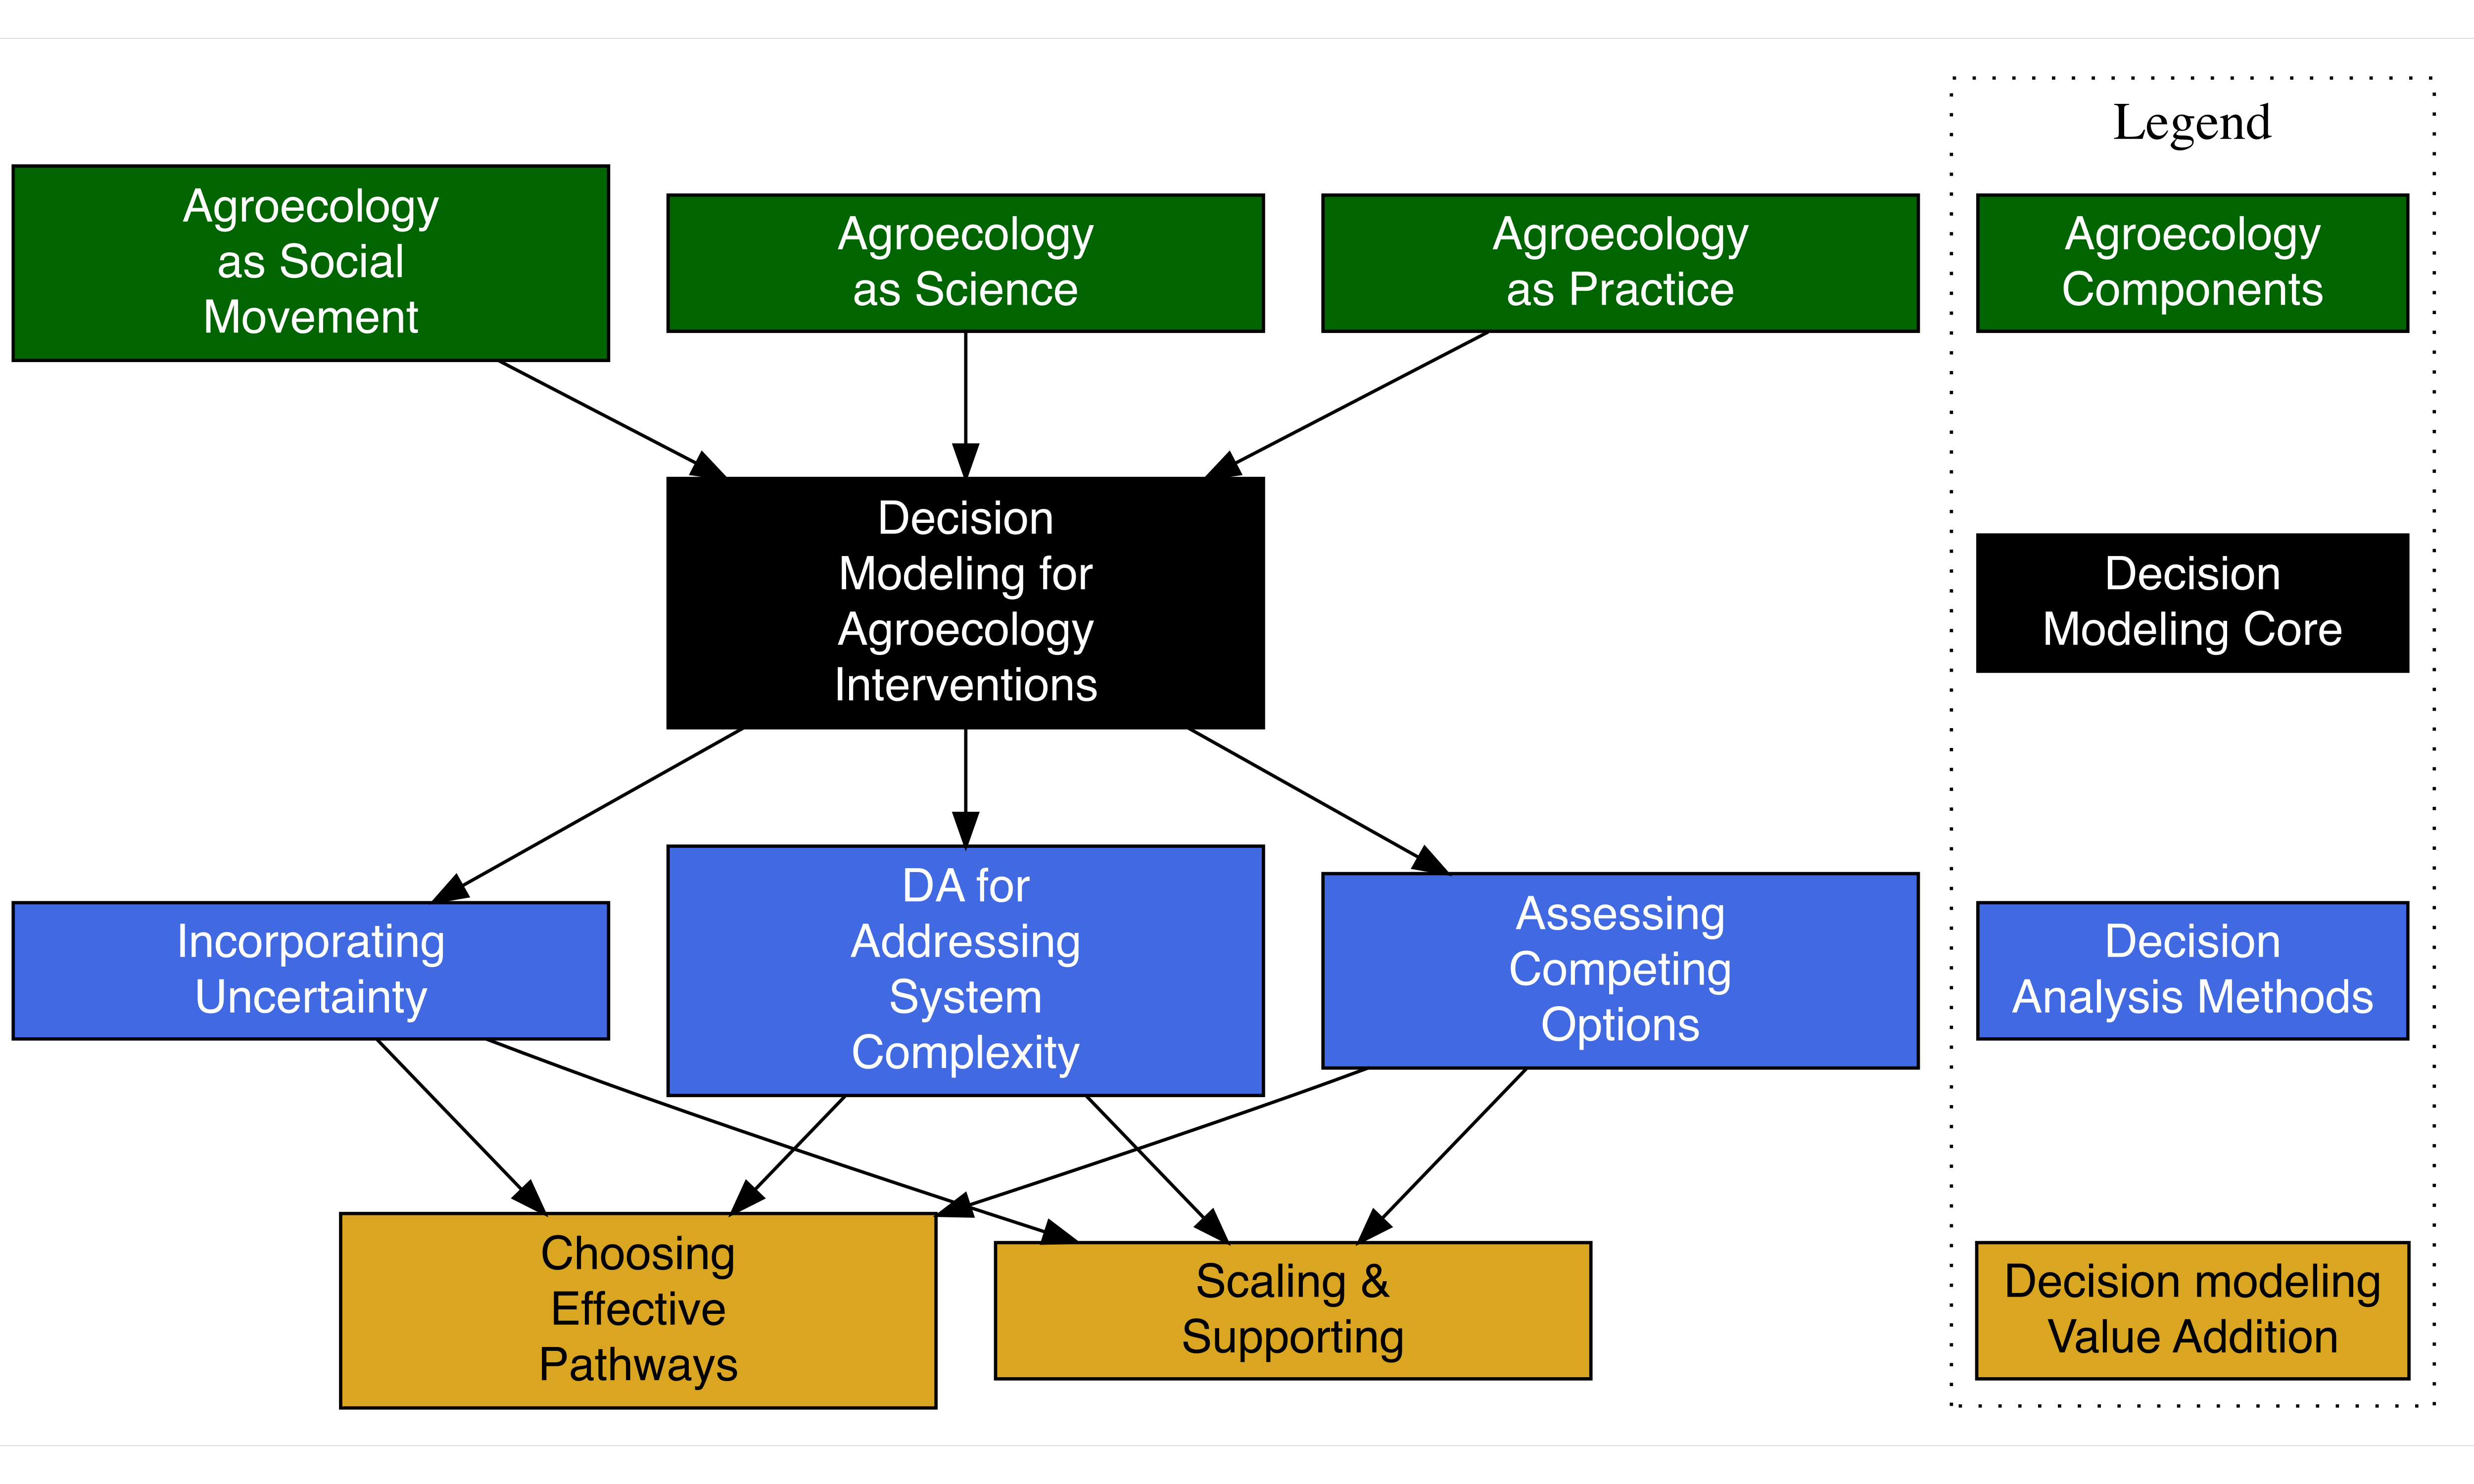
\includegraphics[width=1\linewidth,]{figures/da_agroeco_model} 

}

\caption{\label{fig:da_agroeco_model}Conceptual relationships between decision analytical methods and agroecology—overview of how decision analysis methods can support decision-making for agroecology interventions (adapted from Whitney et al., 2023).}\label{fig:da_agroeco_model}
\end{figure}

Rather than relying solely on data-driven approaches, my work applies
structured decision-support tools, expert-elicited probabilistic models,
and participatory methodologies to capture local knowledge and decision
constraints. By using Bayesian networks, Monte Carlo simulations and
holistic evaluation frameworks, I facilitate decision-making that
explicitly accounts for trade-offs, uncertainties, and system
interdependencies. This approach has been instrumental in agroforestry
adoption, water resource management, biodiversity conservation, and
climate adaptation, where structured engagement with local communities
enhances the sustainability and scalability of interventions.

The studies presented in this section demonstrate how participatory
decision-support frameworks can integrate expert and local knowledge,
creating a bridge between science, policy, and practice. For example,
stakeholder-driven agro-climate services have been shown to improve the
design and adoption of climate adaptation strategies by aligning
interventions with farmers' lived experiences. Similarly, decision
models applied with smallholder farmers ensure that agroforestry
strategies reflect practical realities rather than abstract theoretical
constructs.

Recognizing the value of Indigenous and local ecological knowledge, my
research also explores ways to integrate traditional farming practices
into structured decision models. Indigenous conservation strategies,
community-led resource management, and localized agroecological
knowledge provide valuable insights that enhance sustainability and
resilience. By embedding these perspectives into decision-analytical
tools, my work contributes to a more inclusive and effective approach to
agroecology.

By emphasizing transdisciplinary collaboration, participatory
engagement, and structured decision analysis, this section highlights
how agroecological interventions can be more effectively designed and
implemented. The following chapters will further explore these themes,
demonstrating how integrating diverse knowledge systems leads to more
adaptive, resilient, and equitable agricultural transitions.

\hypertarget{transdisciplinary-approaches-in-agroecology}{%
\subsection{Transdisciplinary Approaches in
Agroecology}\label{transdisciplinary-approaches-in-agroecology}}

Agroecology requires decision-making frameworks that integrate
ecological, economic, and social dimensions while accounting for
uncertainty and stakeholder priorities. Conventional models often fail
to incorporate expert knowledge and participatory insights, limiting
their applicability. My work applies probabilistic decision analysis,
Bayesian networks, and participatory modeling to develop structured,
expert-driven approaches that enhance agroecological decision-making.

We developed structured decision-support frameworks that integrate
ecological, economic, and social dimensions while addressing uncertainty
and stakeholder priorities in agroecological decision-making.
Conventional models often lack expert knowledge integration and
participatory insights, reducing their relevance for complex
agricultural systems. To address these gaps, we applied probabilistic
decision analysis, Bayesian networks, and participatory modeling to
create structured, expert-driven approaches that

In McGonigle \emph{et al.} (2020) we introduced a knowledge brokering
framework that bridges scientific research, policy development, and
agricultural practice. This framework facilitates landscape-scale
decision-making, ensuring that scientific insights are effectively
translated into practical agroecological policies. We outline a process
for collaboration among researchers, policymakers, and practitioners,
improving stakeholder engagement, decision clarity, and the integration
of agroecological principles. By categorizing policy levers and
interventions, we outlined decision stages within the policy cycle,
linking them to specific decision approaches and tools. By structuring
collaboration between researchers, farmers, and policymakers, we
improved stakeholder engagement, decision clarity, and the co-creation
of sustainable land-use strategies. The framework bridges gaps between
research, policy, and practice, facilitating integrated landscape
management (Fig. \ref{fig:mcgonigle_cycle}).

\begin{figure}[H]

{\centering 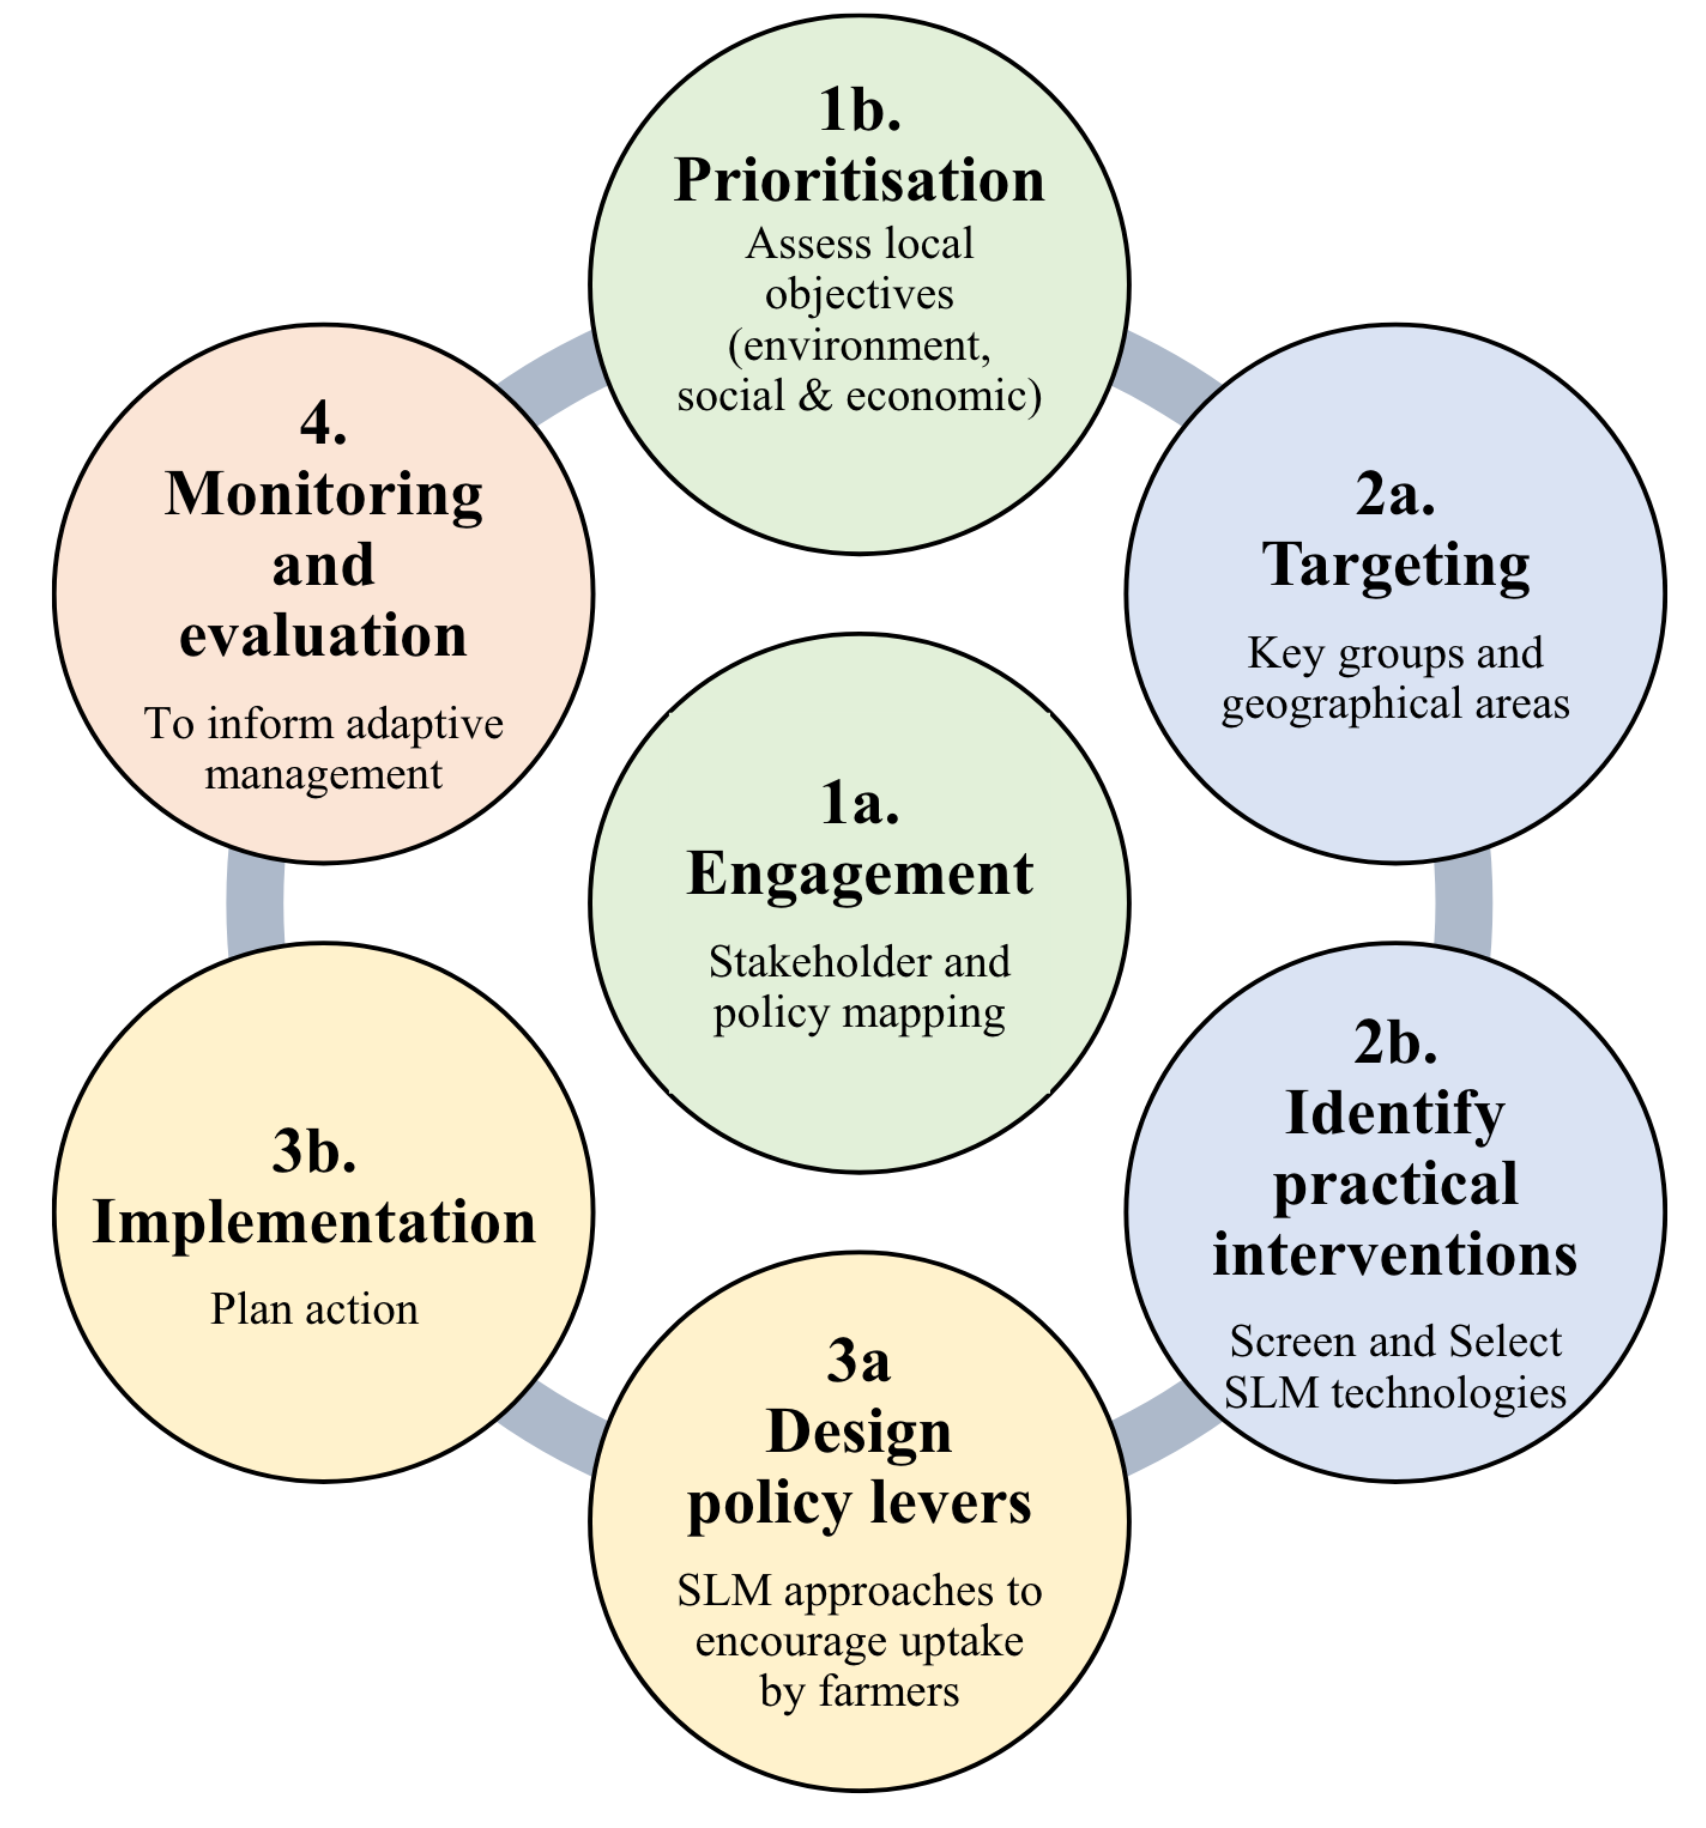
\includegraphics[width=0.5\linewidth,]{figures/mcgonigle_cycle} 

}

\caption{\label{fig:mcgonigle_cycle}An idealised design cycle for integrated landscape management policies and programs. The cycle provides a typology of decisions and design phases to inform seven types of policy decision relating to integrated landscape management (Mcgonigle et al. 2020).}\label{fig:mcgonigle_cycle}
\end{figure}

We also sought to explore meaningful pathways to managing stakeholder
involvement. In Luu \emph{et al.} (2024b), we designed a stakeholder
engagement framework for agro-climate services, using participatory
methods to improve decision-making, service scalability, and long-term
adoption. In Do \emph{et al.} (2020), we applied probabilistic decision
modeling with Vietnamese smallholder farmers, integrating
expert-elicited probabilities to assess agroforestry adoption risks.
This structured approach enabled reasoning under uncertainty, ensuring
that agroecological interventions account for long-term ecological and
economic trade-offs. By co-developing decision models with farmers, we
improved model relevance, local ownership, and the practical
applicability of agroforestry decision-support tools. We developed a
stakeholder-driven framework for agro-climate services (ACS),
demonstrating how collaborative decision-making improves adoption and
impact. By engaging farmers, researchers, and policymakers in
co-creating service delivery models, we ensured that ACS are not only
technically viable but also aligned with real-world agricultural needs
(Fig. \ref{fig:luu_stakeholders}).

\begin{figure}[H]

{\centering 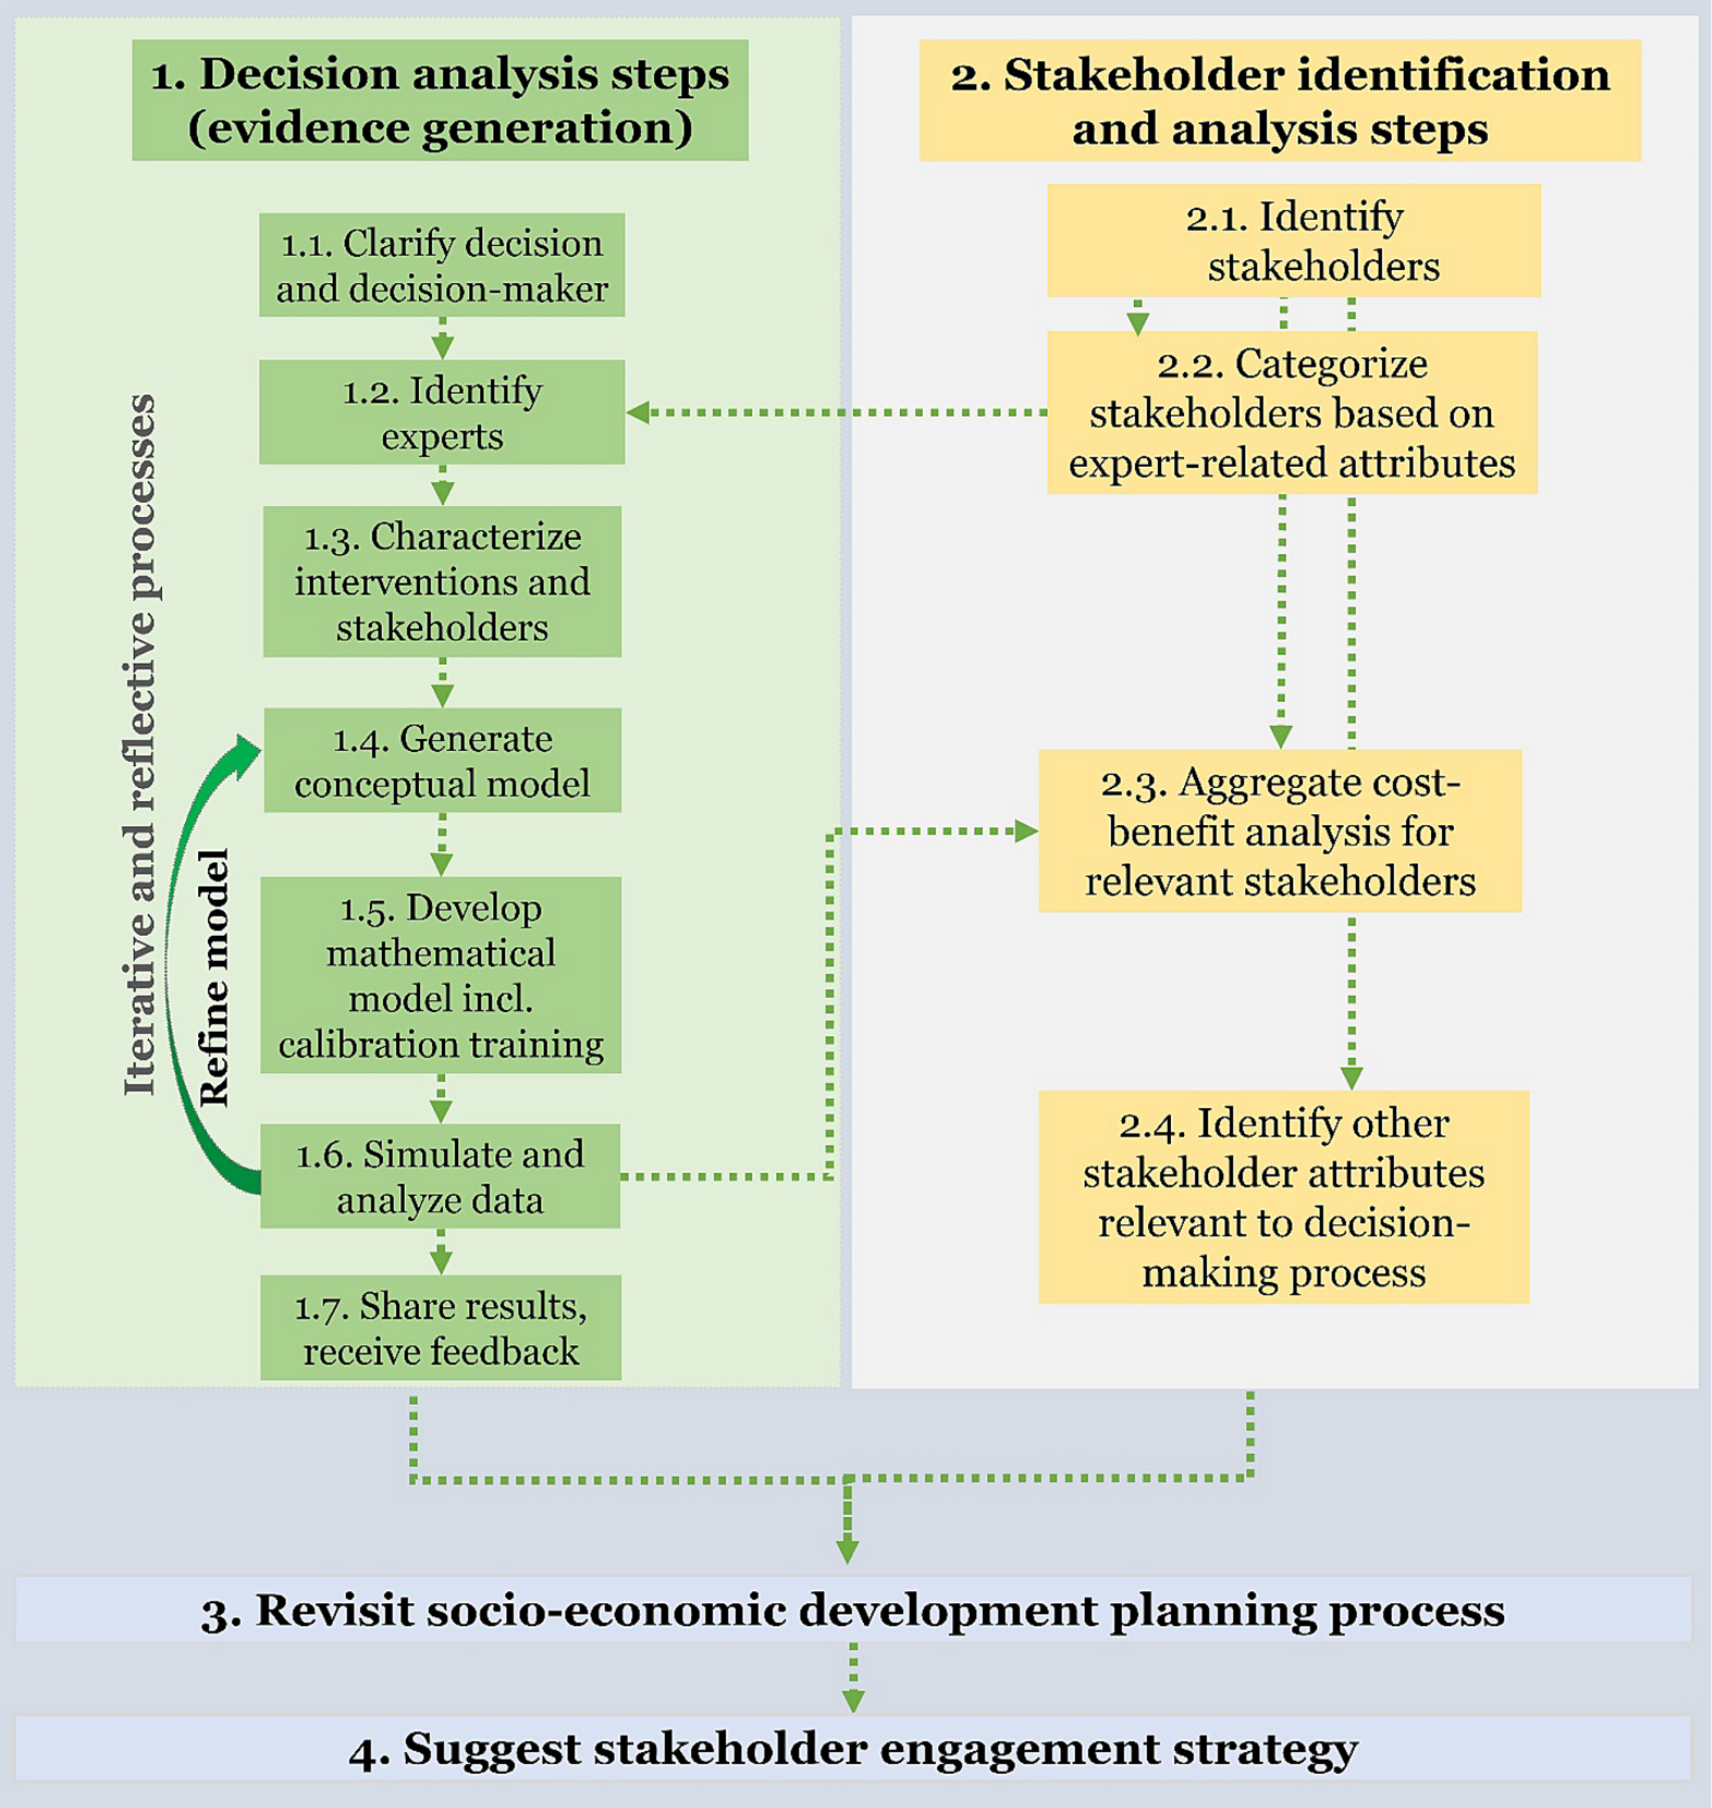
\includegraphics[width=0.8\linewidth,]{figures/luu_stakeholders} 

}

\caption{\label{fig:luu_stakeholders}Approach to engaging stakeholders in agro-climate service planning. The methodological steps of decision analysis in the context of ACS (Luu et al., 2024).}\label{fig:luu_stakeholders}
\end{figure}

We continuously refine transdisciplinary decision models to balance
expert-driven probabilistic reasoning with participatory knowledge
elicitation, ensuring that decision-support tools remain adaptive,
scalable, and relevant to diverse agricultural contexts. While
probabilistic models structure uncertainty and trade-offs, effective
decision-making requires ongoing stakeholder engagement and iterative
model updates.

In Luu \emph{et al.} (2024a), we applied an adaptive decision framework
to improve agro-climate service adoption, incorporating farmer learning,
feedback loops, and iterative refinements. This demonstrated how
decision models must evolve based on real-world implementation, ensuring
that predictions remain actionable and aligned with changing
environmental and socio-economic conditions.

\hypertarget{co-creating-solutions-through-participatory-methods}{%
\subsection{Co-Creating Solutions Through Participatory
Methods}\label{co-creating-solutions-through-participatory-methods}}

Agroecological transitions require inclusive and participatory
approaches to ensure that interventions are effective, scalable, and
aligned with local realities. Many policies and models fail to integrate
farmer knowledge, Indigenous perspectives, and community-driven
adaptation strategies, leading to interventions that lack long-term
relevance and impact. Conventional expert-driven models often fail to
capture context-specific decision factors, making them difficult to
implement at the community level. This section explores how
participatory modeling and knowledge co-production enhance
decision-making, enabling stakeholders to develop actionable and locally
grounded strategies.

Decision analysis methods play a crucial role in prioritizing
agroecological interventions by accounting for environmental, economic,
and social trade-offs. Conventional approaches frequently neglect
uncertainty and multi-criteria decision-making, which can result in
interventions that fail to balance sustainability with economic
viability. By integrating probabilistic reasoning and structured
trade-off analysis, we developed decision-support tools that guide
sustainable agricultural practices while remaining adaptive to local
conditions.

Indigenous knowledge systems provide invaluable insights into
biodiversity conservation, soil health, and agroecological resilience,
yet they are often marginalized in formal decision models. Many top-down
conservation and agricultural policies fail to recognize the ecological
significance and practical applicability of Indigenous knowledge,
limiting their effectiveness and adoption. To address this challenge,
our work integrates Indigenous ecological knowledge into structured
decision-support frameworks, ensuring that interventions remain
culturally relevant and ecologically sustainable.

By embedding Indigenous conservation strategies and agroforestry
practices into probabilistic decision frameworks, we ensure that
traditional land-use planning and biodiversity conservation methods
inform sustainable agricultural management. Conventional decision models
frequently exclude local and Indigenous expertise, limiting their
relevance in complex socio-ecological systems. Incorporating
expert-elicited probabilities from Indigenous knowledge holders enhances
the applicability of decision-support tools, making them more reflective
of traditional resource management strategies. The integration of
Indigenous knowledge strengthens agroecological interventions by making
them culturally appropriate and ecologically sustainable. Studies such
as Oluoch \emph{et al.} (2023) and Tabuti \emph{et al.} (2022) highlight
how local conservation strategies and traditional agroforestry practices
can be incorporated into decision models, ensuring that interventions
are socially embedded and community-led.

In Oluoch \emph{et al.} (2023), we employed participatory decision
models to capture Indigenous perceptions of wild edible plants,
highlighting their cultural, nutritional, and ecological importance.
This approach ensured that local resource-use strategies were embedded
within conservation planning, aligning scientific models with community
priorities. Similarly, in Tabuti \emph{et al.} (2022), we applied
structured frameworks to assess community-led conservation of woody
species, demonstrating how Indigenous land-use practices contribute to
biodiversity conservation and sustainable agroforestry management. We
explored the diversity and uses of woody species in Awach Sub-county,
Uganda, through a participatory research approach that actively involved
local people in the study process. We conducted household interviews
with randomly selected informants, ensuring that a broad range of
perspectives was included. By applying exploratory quantitative
ethnobotany analysis, we captured both the material contributions and
cultural significance of 64 multipurpose tree species valued by the
community.

This participatory approach allowed us to document the values for which
local people maintain and protect woody species, offering insights into
their ecological and socio-economic importance. Informants shared
knowledge on tree management, challenges such as pests, diseases, and
infrastructure limitations, and strategies for sustainable species use.
The engagement of local stakeholders was central to identifying policy
mechanisms that support tree establishment and conservation in the
region and across sub-Saharan Africa.

To further analyze differences in tree species preferences along
socio-demographic gradients, we ran Nonmetric Multidimensional Scaling
(NMDS) ordination as an additional exploratory tool (Fig.
\ref{fig:tabuti_priority_2022_NMDS}). This approach helped visualize how
preferences varied based on factors such as income sources, village of
origin, sex, age, and household size. We tested for differences using
Permutational Multivariate Analysis of Variance (PERMANOVA), followed by
pairwise comparisons. These methods provided deeper insights into the
social dimensions of tree use and conservation decisions within the
community. By integrating participatory research with quantitative
ethnobotany, our study highlights the importance of local knowledge in
shaping sustainable land management strategies. The findings underscore
the need for policies that recognize and support community-led
conservation efforts, ensuring that local priorities drive reforestation
and biodiversity conservation initiatives.

Figure \ref{fig:tabuti_priority_2022_NMDS} shows NMDS and PERMANOVA and
pairwise comparisons results for 121 informants in Awach subcounty, Gulu
District, Uganda. The figure visualizes preferences for 64 woody
species, with a stress value of 0.18.

\begin{figure}[H]

{\centering 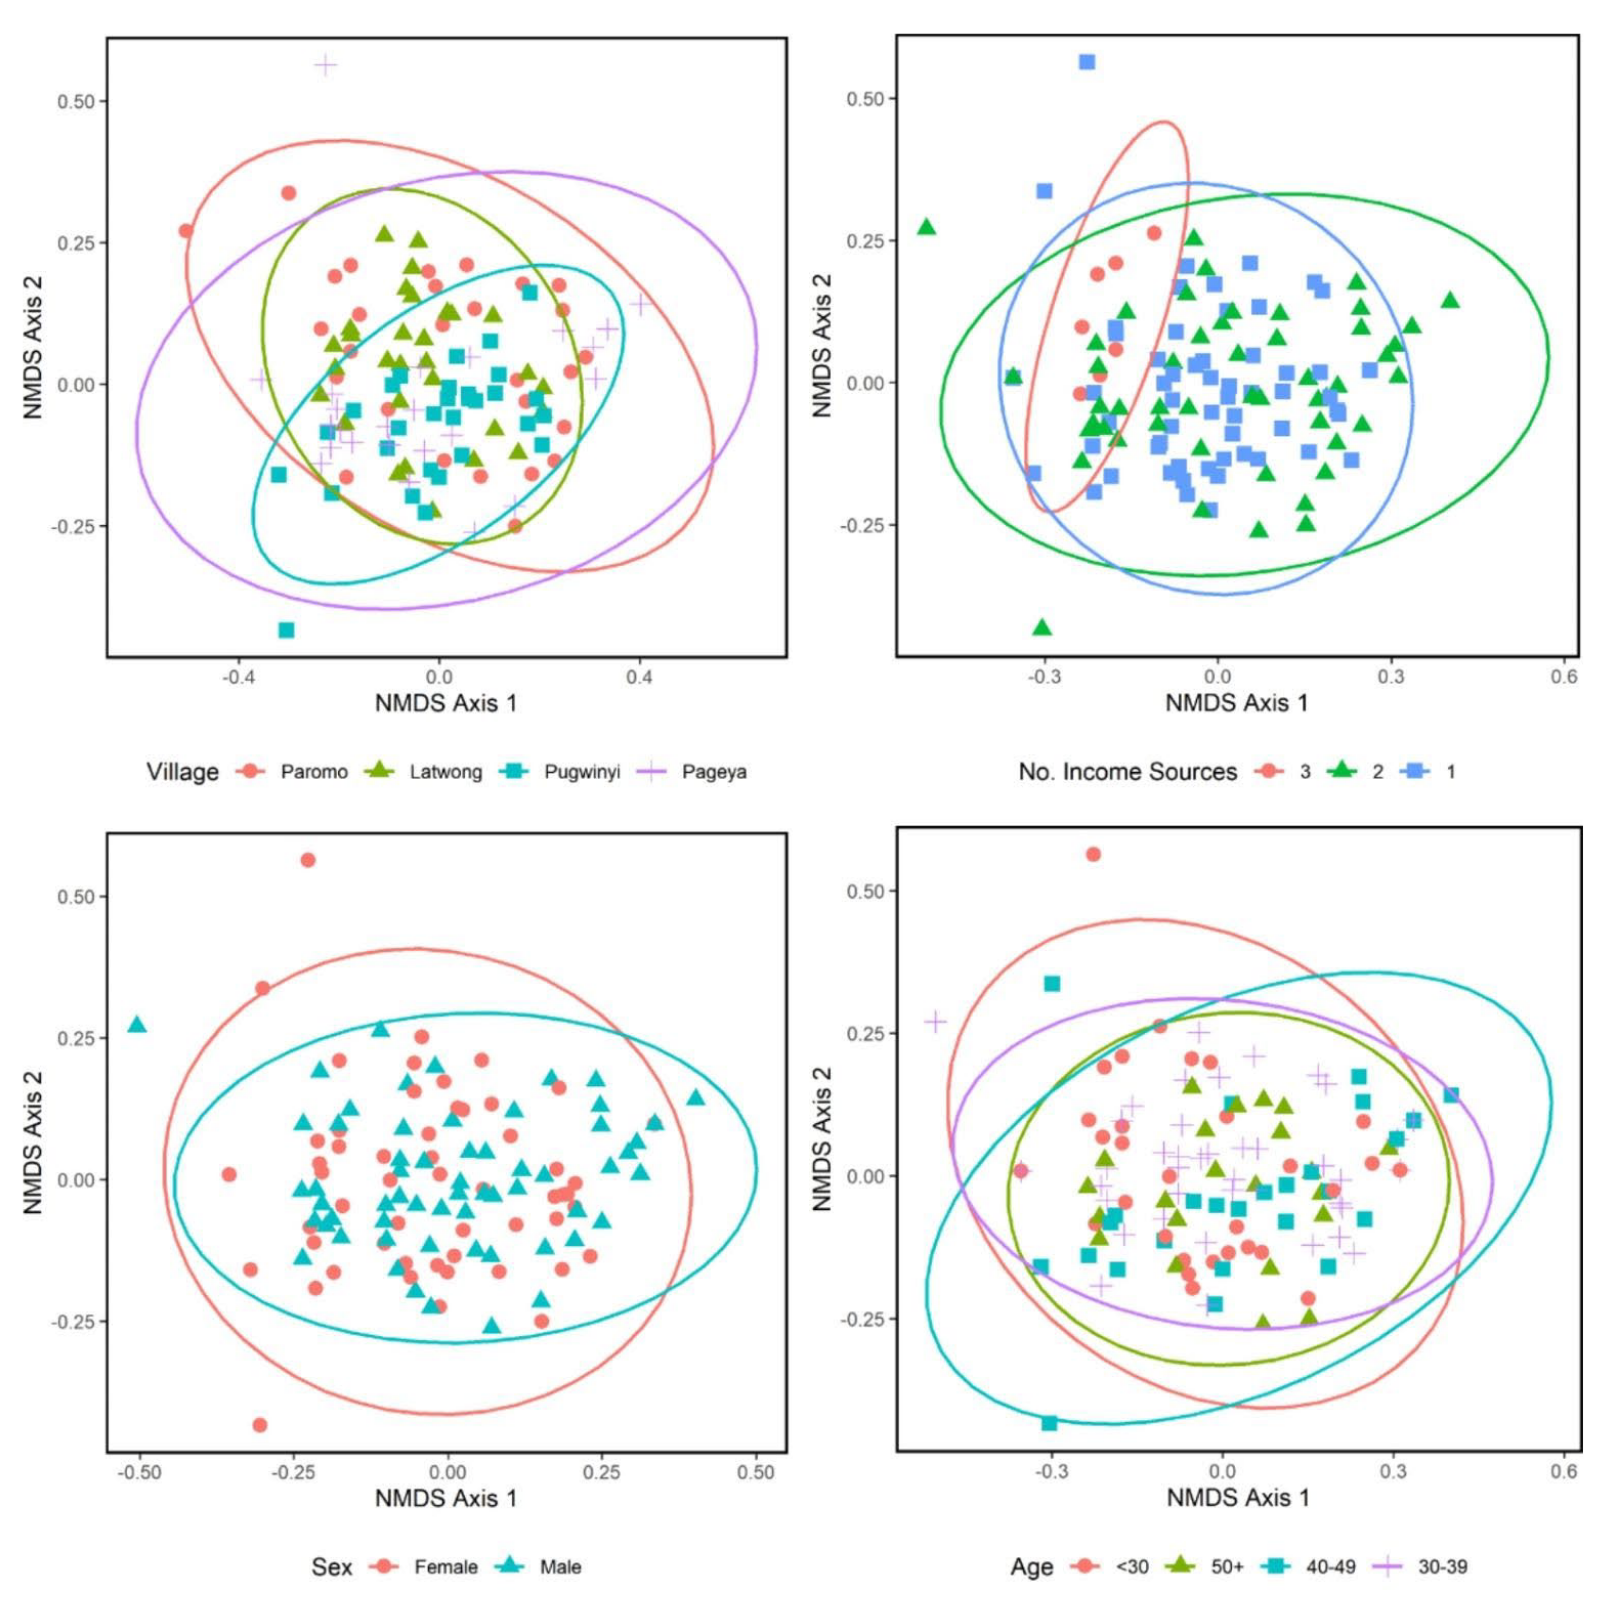
\includegraphics[width=0.8\linewidth,]{figures/tabuti_priority_2022_NMDS} 

}

\caption{\label{fig:tabuti_priority_2022_NMDS}Nonmetric Multidimensional Scaling ordination for tree species preferences based on socio-demographic factors (Tabuti et al., 2022).}\label{fig:tabuti_priority_2022_NMDS}
\end{figure}

Participatory methods further enhance the integration of local expertise
into agroecological decision-making. The scalability and adaptability of
these models are critical for advancing agroecology. In Luu \emph{et
al.} (2022), we investigated the challenges associated with scaling
agro-climate services (ACS) in Vietnam, using decision analysis to
identify leverage points that improve service adoption. Our study
examined how stakeholder engagement could enhance the scalability and
effectiveness of these interventions.

Farmers in Vietnam are highly sensitive to climate variability, and the
lack of timely, actionable climate-informed agricultural advice leads to
significant input and yield losses. Development organizations, including
CARE in Vietnam, have provided ACS on a limited scale, advocating for
government support in scaling these services. However, a large-scale
rollout could strain financial and human resources. Given the inherent
uncertainty in weather risks and the benefits of ACS, we applied a
decision analysis approach to conduct an ex-ante cost-benefit analysis
of four candidate interventions for scaling ACS in Dien Bien District.

A key feature of our approach was the active participation of farmers
and local stakeholders in designing and evaluating the interventions. We
worked closely with CARE in Vietnam, Dien Bien government staff, and
agricultural experts to ensure that decision models captured the
realities faced by smallholder farmers (Fig.
\ref{fig:luu_decision_2022_model}). Through participatory workshops and
structured elicitation processes, farmers contributed their knowledge
and experiences, shaping the conceptual models and informing the
probabilistic simulations used in our analysis.

Figure \ref{fig:luu_decision_2022_model} illustrates the structure and
implementation of ACS interventions, highlighting key activities,
stakeholder interactions, and information flows. The black arrows
represent the movement of information between stakeholders. Green boxes
indicate core activities common to all four interventions, while yellow
boxes with numbers specify intervention-specific actions. Stakeholders
are identified within winged parentheses to emphasize their roles in the
decision-making process

\begin{figure}[H]

{\centering 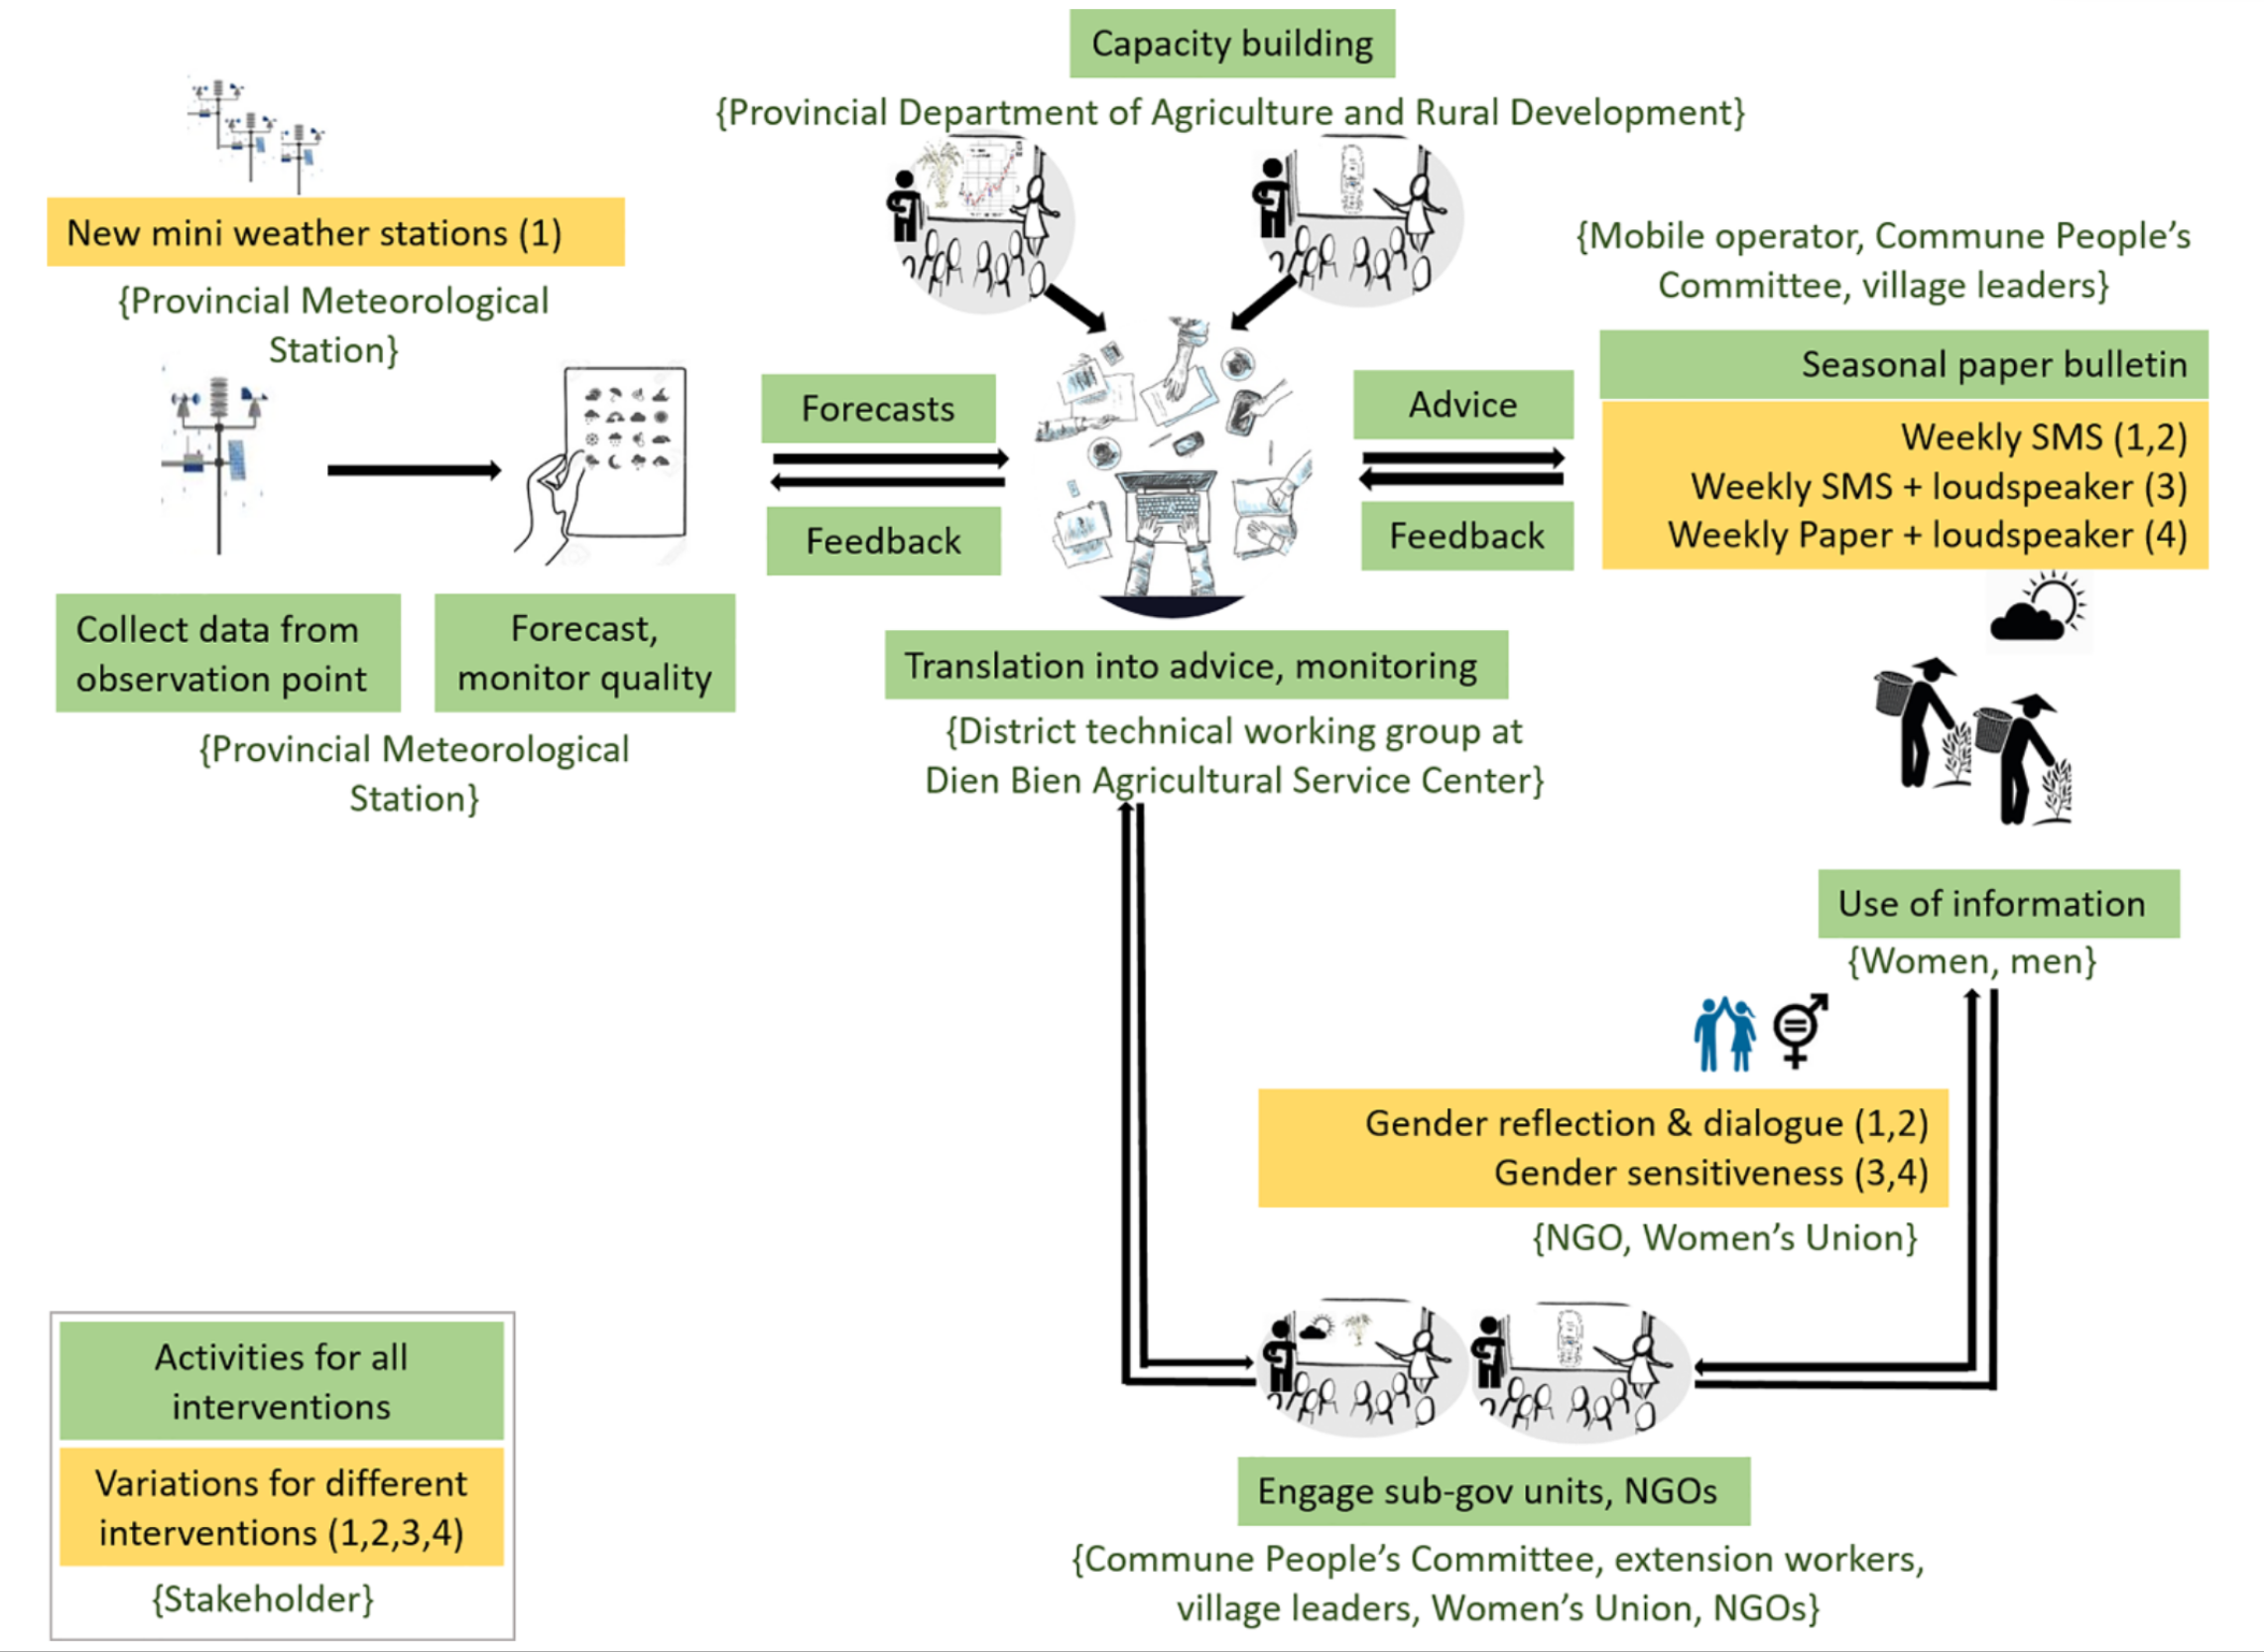
\includegraphics[width=0.8\linewidth,]{figures/luu_decision_2022_model} 

}

\caption{\label{fig:luu_decision_2022_model}Overview of Four Agro Climate Service (ACS) Interventions in Dien Bien District, Vietnam (Luu et al 2022).}\label{fig:luu_decision_2022_model}
\end{figure}

Our results indicated a high likelihood of ACS interventions providing
net benefits. Investments in ACS were projected to yield high returns,
between 1.45 and 16.02 USD per 1 USD invested. These findings offer a
strong foundation for decision-making, advocating for the replacement of
deterministic assessments with probabilistic approaches in evaluating
complex and uncertain development planning decisions. Importantly, the
participatory nature of the research ensured that the decision-support
tools developed were both scientifically robust and practically relevant
to the communities they aimed to serve.

Stakeholder-driven agro-climate services were shown to improve the
design, scalability, and adoption of climate adaptation strategies by
aligning interventions with farmers' lived experiences. By combining
stakeholder engagement with probabilistic modeling, we identified key
barriers to adoption and pathways for improving service delivery.

In Do \emph{et al.} (2020) we represented uncertainties in the model by
expressing all variables as probability distributions derived from
expert assessments. To ensure inclusivity, we designed the expert
elicitation process as an iterative, participatory engagement with
stakeholders. Calibration training sessions improved the accuracy of
uncertainty estimates while integrating diverse perspectives. Unlike
conventional expert elicitation, our approach included feedback loops
where farmers and stakeholders refined model inputs. Participatory
workshops facilitated knowledge co-production, allowing local
stakeholders to adjust expert assessments based on lived experience,
ensuring alignment with real-world constraints. After training, experts
and stakeholders provided 90\% confidence intervals and distribution
shapes for all input variables. This collaborative approach increased
accuracy and fostered trust and ownership over decision models. By
embedding participatory elements into probabilistic modeling, we
enhanced the relevance, transparency, and legitimacy of decision-support
frameworks in agroecological transitions.

By bridging local and Indigenous ecological knowledge with probabilistic
decision models, our research supports co-created agroecological
solutions that are both scientifically rigorous and socially inclusive.
These studies highlight the necessity of integrating Indigenous
perspectives into agricultural decision-making to ensure that local
priorities and traditional practices inform sustainable food systems.

Beyond probabilistic modeling, our research underscores the importance
of stakeholder engagement and participatory knowledge co-production.
Many agroecological interventions fail because they do not integrate
local expertise or address real-world decision constraints. To overcome
this, we develop participatory decision-support frameworks that
incorporate expert and stakeholder knowledge into structured
probabilistic reasoning, making them more effective in real-world
agroecological transitions.

By leveraging expert knowledge, structured probabilistic reasoning, and
participatory decision-making, our work advances methods for navigating
uncertainty in agroecology. These approaches ensure that
decision-support tools align with both scientific principles and the
expertise of practitioners, policymakers, and communities, providing
actionable insights for sustainable agricultural transitions.

\hypertarget{assessing-agroecological-interventions-using-holistic-evaluation-frameworks}{%
\subsection{Assessing Agroecological Interventions Using Holistic
Evaluation
Frameworks}\label{assessing-agroecological-interventions-using-holistic-evaluation-frameworks}}

Assessing agroecological interventions requires decision-support
frameworks that account for uncertainty and trade-offs across
ecological, economic, and social dimensions. Traditional impact
assessments often rely on deterministic models, which fail to capture
variability in farming systems, environmental responses, and long-term
policy effects. We address this challenge by applying probabilistic
decision analysis, integrating expert-elicited probabilities and
participatory modeling to improve the assessment of agroecological
interventions.

By combining structured expert knowledge with Monte Carlo simulations,
Bayesian networks, and scenario-based modeling, we project intervention
outcomes under varying conditions. This approach ensures decision-making
processes remain robust, adaptable, and reflective of real-world
uncertainties. Additionally, participatory modeling enhances this
framework by incorporating farmers' and stakeholders' perspectives.
Conventional top-down approaches often overlook local decision factors
that shape intervention success. By co-designing and validating decision
models with stakeholders, we align agroecological assessments with local
needs, fostering ownership and increasing the likelihood of adoption.

In Whitney \emph{et al.} (2023) and Fernandez \emph{et al.} (2022), we
demonstrate how decision analysis methods evaluate agroecological
transitions, balancing short-term implementation challenges and
long-term sustainability. Similarly, Do \emph{et al.} (2020) and Tabuti
\emph{et al.} (2022) highlight the integration of local ecological
knowledge into structured decision frameworks for land-use planning and
agroforestry management. Our work in Luu \emph{et al.} (2024a) and
Netter \emph{et al.} (2022) further illustrates how participatory
approaches enhance the scalability of agro-climate services and the
evaluation of voluntary carbon offset certifications.

A key component of assessing agroecological interventions is
understanding the decision-making processes that influence their
adoption and impact. In Luu \emph{et al.} (2024a), we developed a
framework to analyze the adoption dynamics of ACS (Fig.
\ref{fig:Luu_et_al_2024_hypothesis}). This framework captures how
farmers' perceptions of climate risks shape their need for ACS, their
engagement with information, and their subsequent adoption decisions.
Our analysis distinguishes between Village Savings and Loan Association
(VSLA) members and non-VSLA farmers, assessing how structured financial
and knowledge-sharing networks influence ACS uptake. Farmers who adopt
ACS may confirm their continued need, reject specific recommendations,
or recommend ACS to peers. This participatory approach highlights the
role of farmer networks in shaping adoption pathways and underscores the
importance of aligning agroecological interventions with local
decision-making processes (Fig. \ref{fig:Luu_et_al_2024_hypothesis}).

\begin{figure}[H]

{\centering 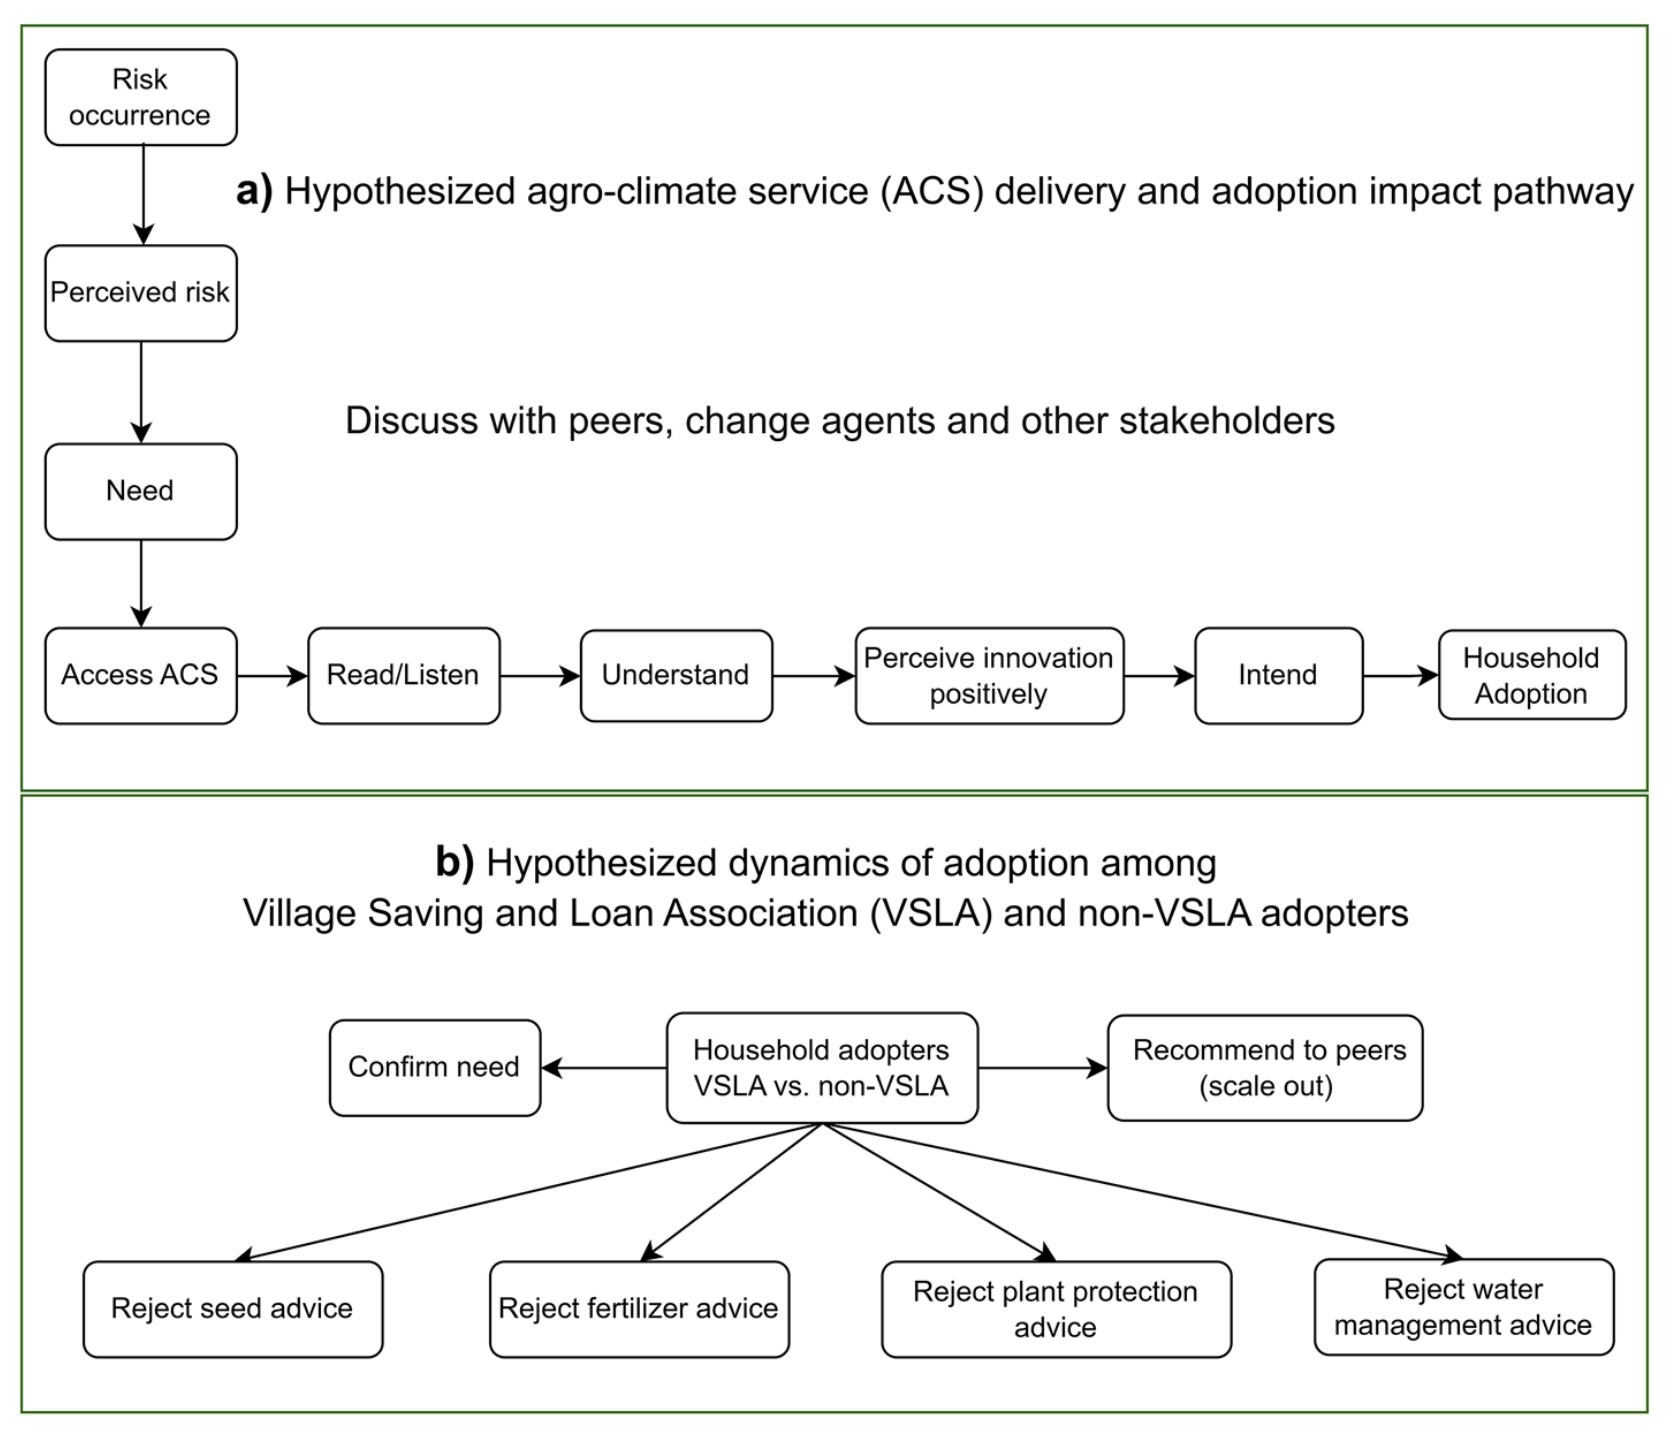
\includegraphics[width=1\linewidth,]{figures/Luu_et_al_2024_hypothesis} 

}

\caption{\label{fig:mcgonigle_knowledge_toolkit}Hypothesized agro-climate service (ACS) adoption pathways in Muong Phang and Pa Khoang communes, Dien Bien District, Vietnam (Luu et al. 2024). (a) Sequential decision-making process from climate risk perception to ACS adoption. (b) Adoption dynamics among Village Savings and Loan Association (VSLA) members and non-VSLA farmers, highlighting pathways for confirming need, recommending ACS, or rejecting specific advice on seeds, fertilizer, plant protection, and water management (Luu et al. 2024).}\label{fig:Luu_et_al_2024_hypothesis}
\end{figure}

Our analysis contributes to a broader understanding of participatory
decision-making in agroecology. By quantifying adoption rates and
decision pathways, we provide evidence-based recommendations for scaling
ACS and improving their accessibility to smallholder farmers.

By integrating trade-offs between ecological resilience, economic
feasibility, and social outcomes, we enhance evidence-based
decision-making for sustainable agricultural transitions. Our research
demonstrates how probabilistic decision models improve impact
assessments, ensuring agroecological interventions are evaluated within
a structured, uncertainty-aware framework that incorporates stakeholder
perspectives and adaptive management strategies.

\hypertarget{bridging-science-policy-and-practice-in-agroecology}{%
\subsection{Bridging Science, Policy, and Practice in
Agroecology}\label{bridging-science-policy-and-practice-in-agroecology}}

Our research demonstrates how probabilistic decision models improve
agroecological decision-making by systematically addressing uncertainty
and trade-offs. By integrating expert-elicited probabilities into
structured frameworks, we enhance the assessment of agroecological
interventions, ensuring that decision-support tools reflect real-world
constraints and variability.

Spatial models and Bayesian networks further strengthen agroecological
assessments by improving land-use classification and mapping of complex
agroecosystems. Liman Harou \emph{et al.} (2020) and Liman Harou
\emph{et al.} (2021) applied Bayesian networks and remote sensing to
develop probabilistic spatial models, offering more accurate
classifications of flood-based farming systems and land-use transitions.

Participatory decision-support frameworks have proven essential for
enhancing farmer engagement and policy impact. In Luu \emph{et al.}
(2024b), we demonstrated how stakeholder-driven agro-climate services
improve scalability and adoption, while Do \emph{et al.} (2020) applied
co-created decision models to align agroforestry adoption strategies
with smallholder realities. These approaches ensure that decision models
remain contextually relevant and actionable.

Expanding multi-criteria decision analysis will further improve
trade-off assessments in agroecology, particularly in balancing
production, conservation, and socio-economic factors. Strengthening
science-policy-practice networks will enhance transdisciplinary
collaborations, ensuring that research outputs are effectively
translated into actionable policies. Finally, developing hybrid models
that integrate expert knowledge with select data-driven approaches will
improve decision accuracy and adaptability, supporting scalable and
resilient agroecological transitions.

\newpage

\hypertarget{practical-implications-and-impact}{%
\section{Practical implications and
impact}\label{practical-implications-and-impact}}

Assessing the real-world impact of research in decision science,
agroecology, and environmental policy requires looking beyond academic
citations to direct engagement with policymakers, institutions, and
practitioners. While much of my work advances methodologies for
structured decision-making, several studies have had tangible
applications in policy frameworks, agricultural practices, and
conservation planning. These impacts are reflected in collaborations
with government agencies, NGOs, research institutions, and farming
communities across multiple regions.

Structured decision analysis has provided actionable insights for policy
formulation and institutional decision-making. Our research on
agro-climate services has influenced scaling strategies in Vietnam, with
support from CARE International and the Centre for Community Development
in Dien Bien (Luu \emph{et al.} 2022, 2024a). These decision models have
helped refine government and NGO strategies for delivering
climate-informed agricultural advisory services to smallholder farmers.

Research on sustainability trade-offs in banana production has directly
shaped policy recommendations within the Action Alliance for Sustainable
Bananas (ABNB), facilitated through GIZ (Deutsche Gesellschaft für
Internationale Zusammenarbeit). These findings have been integrated into
standard guidelines for sustainable banana farming (Fernandez \emph{et
al.} 2022).

My work has also directly engaged government agencies and policymakers.
Studies on agrobiodiversity and land-use and argicultural development
trade-offs have contributed to discussions on sustainable resource
allocation and food system resilience in Uganda's National Planning
Authority (NPA), the Ministry of Agriculture, Animal Industry and
Fisheries (MAAIF), and the Office of the Prime Minister (Whitney
\emph{et al.} 2018b).

Several studies were developed in collaboration with CGIAR (Consultative
Group on International Agricultural Research) centers, including ICRAF
(World Agroforestry), IWMI (International Water Management Institute),
and Bioversity-CIAT, contributing to decision-support frameworks for
sustainable land use, carbon footprint assessments, and agroecological
transitions. Research on agroforestry adoption, carbon sequestration,
and farm management was conducted in partnership with CIFOR-ICRAF
Vietnam and regional networks. These studies guided farmers in Vietnam
and Sub-Saharan Africa in evaluating the trade-offs between agroforestry
adoption, carbon markets, and food production (Kuyah \emph{et al.} 2019;
Do \emph{et al.} 2024). Work on stochastic modeling for irrigation
planning and water management contributed to CGIAR's research agenda on
climate resilience in agriculture (Yigzaw \emph{et al.} 2019; Tamba
\emph{et al.} 2021). Studies on wild edible plants and their role in
food security and climate adaptation were conducted in partnership with
Alliance Bioversity-CIAT, particularly in Kenya's Turkana region (Oluoch
\emph{et al.} 2024). Findings supported conservation planning and local
food security strategies. Research on carbon footprint models and
national-scale sustainability assessments aligned with CGIAR's
Livestock, Climate, and System Resilience (LCSR) Initiative and FAO's
broader sustainability research. This work contributed to livestock
emissions modeling and provided insights for evaluating trade-offs
between agricultural intensification and climate action (Luedeling
\emph{et al.} 2022).

Several studies had direct applications in farm-level decision-making,
influencing risk management, farm planning, and agroforestry adoption
strategies. These applications involved collaborations with farmers,
cooperatives, and research institutions, ensuring that structured
decision analysis was not just theoretical but applied in real-world
agricultural planning. Decision models helped farmers assess
cost-benefit trade-offs for infrastructure investments to mitigate
extreme weather risks in cherry orchards (Rojas \emph{et al.} 2021).
Horticultural Producers in NRW, Germany: Probabilistic models supported
disease management and economic risk assessments in ornamental plant
production. This research was conducted in partnership with Europlant
Canders GmbH, Landwirtschaftskammer Nordrhein-Westfalen, and
Forschungszentrum Jülich (Burbano-Figueroa \emph{et al.} 2022b; Ruett
\emph{et al.} 2022a). Evaluations of voluntary carbon offset projects in
Latin America informed investment decisions in reforestation, ensuring
that decision analysis frameworks were applied to balance economic and
environmental trade-offs (Netter \emph{et al.} 2022).

My research has also contributed to biodiversity conservation, food
security, and the documentation of traditional ecological knowledge,
particularly through collaborations with Indigenous communities and
smallholder farmers. Research on climate risks and wild edible plants
was conducted with community groups in Kenya's Turkana Region, with CIAT
and Bioversity International. Findings supported local conservation
planning and food security strategies (Oluoch \emph{et al.} 2024). Work
on woody species conservation and livelihood resilience was supported by
local research institutions and CIFOR-ICRAF in Uganda, ensuring that
traditional ecological knowledge was integrated into biodiversity
conservation policies (Tabuti \emph{et al.} 2022). Studies on farmer
perceptions of agroforestry adoption and barriers to climate adaptation
in Vietnam were conducted in collaboration with local agricultural
agencies and CIFOR-ICRAF Vietnam (Luu \emph{et al.} 2024a; Do \emph{et
al.} 2024).

Figure \ref{fig:plot_altmetric_data} presents key metrics that capture
the reach and engagement of selected papers across different thematic
areas. These metrics reflect not only academic recognition through
citations but also broader engagement in policy, stakeholder
involvement, and public discourse. Papers are categorized into five
thematic areas: Biodiversity Conservation, Climate Change Mitigation and
Adaptation, Livelihoods and Socio-Economic Impact, Stakeholder and
Community Engagement, and Sustainability. x-axis shows four key impact
metrics: Altmetric Percentile (relative ranking of a paper's Altmetric
Score compared to similar research, aggregated from various online
sources, including news articles, blogs, policy documents, and social
media), Citations (extracted from Google Scholar), Mentions (total
number of online references to a paper across various platforms,
including news articles, policy documents and social media), Readers
(count of users who have saved the paper in reference management
platforms). Each cell contains the value of the corresponding metric.
The numbers are color-coded within each metric to highlight relative
differences among papers.

\begin{figure}[H]

{\centering 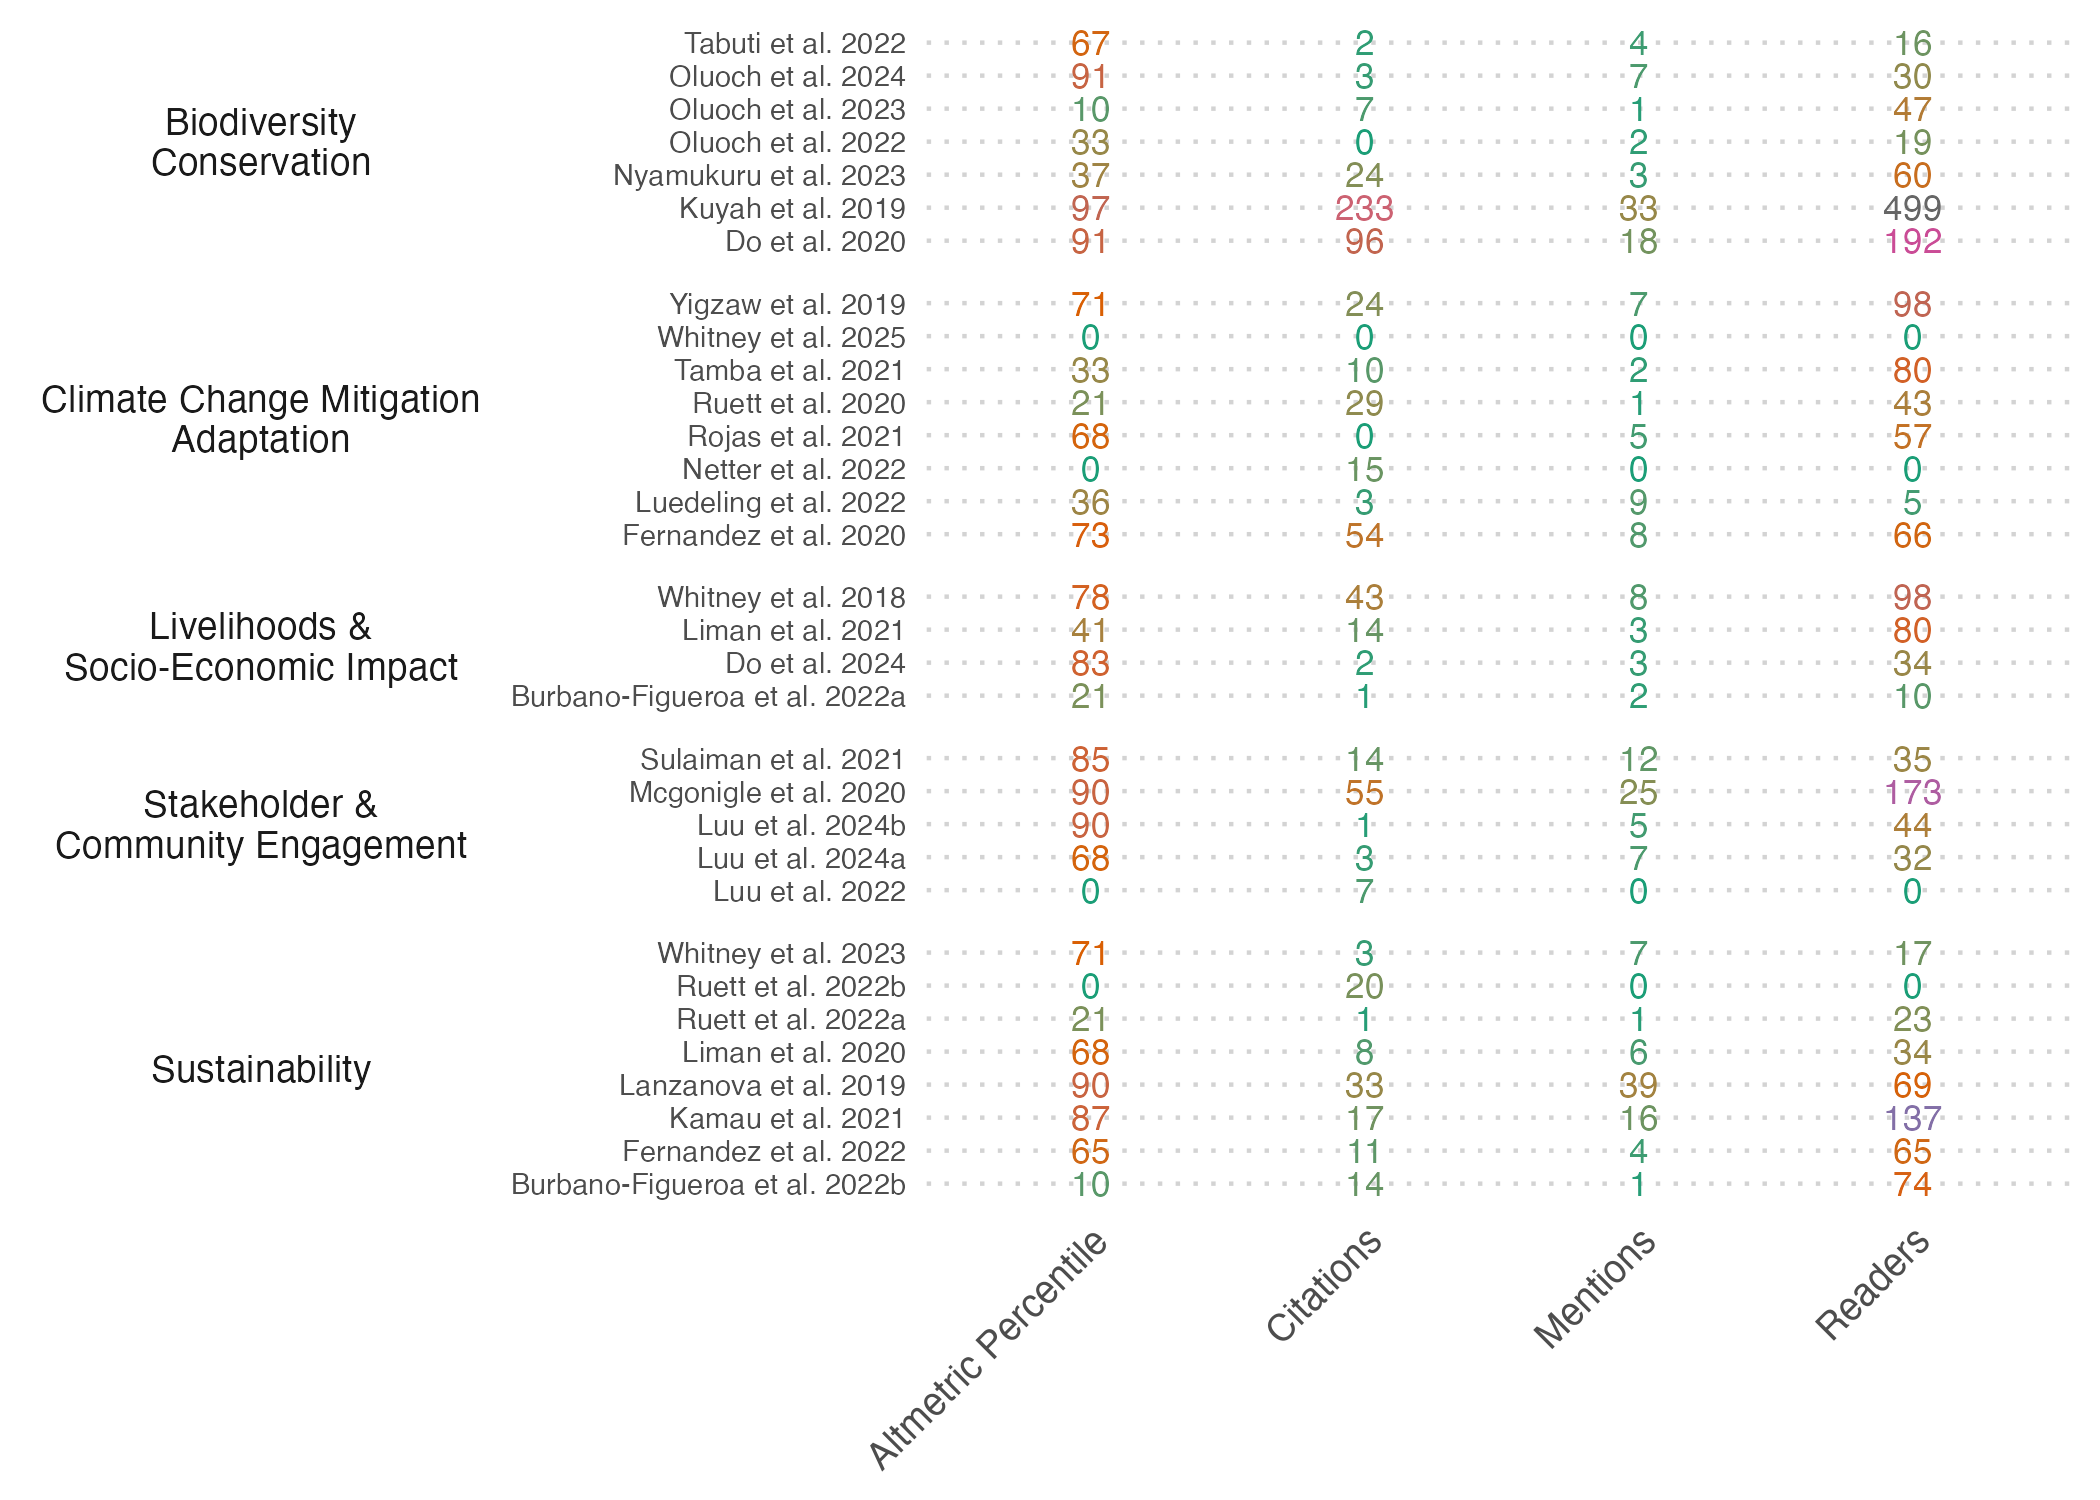
\includegraphics[width=1\linewidth,]{figures/plot_altmetric_data} 

}

\caption{\label{fig:plot_altmetric_data}Altmetric and citation metrics for selected papers, grouped by thematic area.}\label{fig:plot_altmetric_data}
\end{figure}

Beyond academic impact, my research has gained public visibility through
outreach, open-access platforms, and direct engagement with non-academic
audiences (Fig. \ref{fig:plot_altmetric_data}). At least two studies
have been cited in Wikipedia entries related to agroecology and
sustainability, demonstrating a contribution to public discourse on
climate and food security. Research findings have been disseminated
through invited talks, policy workshops, and decision-support training
programs for farmers in NRW, Vietnam, and Uganda. These sessions have
provided practical tools for decision-making in agroecology,
agroforestry, and farm risk management. Many of these studies have
directly involved farmers, conservation practitioners, and policy
advisors, ensuring that probabilistic modeling and decision analysis
frameworks are applied beyond academic research. While these
contributions highlight tangible applications, the direct uptake of
decision models in policy and practice remains variable. Factors such as
institutional constraints, political shifts, and stakeholder priorities
influence whether structured decision analysis is fully integrated into
real-world decision-making.

Some studies, such as those on climate risk management for cherry
orchards and carbon offset strategies, have had clear pathways to
adoption. Others, particularly those focusing on probabilistic modeling
improvements and uncertainty quantification, remain foundational
contributions that require further application through pilot programs,
policy initiatives, or stakeholder engagement. Despite these challenges,
the research provides a critical framework for structured
decision-making, with ongoing efforts to enhance its applicability
across agricultural, environmental, and policy contexts.

\newpage

\hypertarget{conclusion-and-outlook}{%
\section{Conclusion and Outlook}\label{conclusion-and-outlook}}

In this habilitation, I have demonstrated how decision analytical
methods and probabilistic modeling provide structured approaches to
address the complex challenges of agroecology and sustainable
development. By systematically applying these techniques, I have
identified key trade-offs, risks, and uncertainties that shape
agricultural decision-making, policy design, and environmental
management. These methods have allowed me to integrate expert knowledge,
participatory insights, and probabilistic reasoning, ensuring that
agroecological interventions are both scientifically robust and
practically viable. In an era of escalating global change, these
methodologies provide practical, scalable, and adaptive frameworks that
support resilient food systems and informed decision-making across
diverse agricultural landscapes. My work generates insights into how
sustainable development can be achieved through transdisciplinary
modeling, offering theoretical advances in decision theory and practical
tools for policymakers.

My research has shown that uncertainty is an inherent feature of
agroecological systems, and decision-support tools must account for this
variability. Through the application of Bayesian networks, Monte Carlo
simulations, and structured decision analysis, I have refined methods
for evaluating interventions under conditions of incomplete information.
By combining these probabilistic models with stakeholder engagement and
participatory frameworks, I have strengthened the alignment between
scientific modeling and real-world agricultural realities, making
decision-support tools more accessible and actionable.

While my work so far has mainly focused on case studies, the models are
designed to be scalable and applicable to other regions facing similar
challenges. The decision-support framework can be adapted to other
contexts, allowing for global applications that are tailored to local
conditions. This is particularly important for smallholder farmers and
Indigenous communities, whose livelihoods are directly impacted by both
climate change and conservation policies. I ensure that the solutions
are locally grounded---reflecting the unique social, ecological, and
economic conditions of each community. My work has the potential to make
a lasting impact both at the local level, by improving livelihoods, and
at the global level, by informing international development and
conservation strategies.

\hypertarget{contributions-to-agroecology}{%
\subsection{Contributions to
Agroecology}\label{contributions-to-agroecology}}

My research has demonstrated how formal decision analysis improves the
efficacy of agroecological interventions by structuring uncertainty,
trade-offs, and stakeholder priorities into a coherent framework. By
applying Bayesian networks, Monte Carlo simulations, and structured
decision models, I have developed approaches that facilitate
evidence-based decision-making and improve the practical applicability
of agroecological strategies. These methods ensure that decision-support
tools align with both scientific principles and local agricultural
realities.

I have applied probabilistic tools to manage uncertainties in
agricultural decision-making, illustrating how expert-elicited
probabilities enhance policy and intervention assessments. By
integrating stochastic models and scenario-based approaches, my work has
supported resilient and adaptive agricultural strategies, providing
quantitative insights into intervention outcomes and enabling
stakeholders to make uncertainty-aware decisions in dynamic
agroecosystems.

My research has also emphasized the importance of sustainable species
prioritization, ecosystem management, and conservation planning in
agroecological systems. Through allometric models, restoration
simulations, and probabilistic assessments, I have quantified ecological
trade-offs and benefits, helping guide conservation efforts,
reforestation strategies, and agroforestry interventions. These
contributions provide structured approaches to balancing biodiversity
conservation with agricultural productivity, ensuring that
sustainability remains central to agroecological decision-making.

\hypertarget{future-research-directions}{%
\subsection{Future Research
Directions}\label{future-research-directions}}

Looking forward, I aim to further advance transdisciplinary decision
modeling to scale agroecological solutions and inform policy frameworks.
The research will focus on refining hybrid models that integrate
expert-elicited probabilities with emerging datasets, expanding
multi-criteria decision analysis for more holistic trade-off
assessments, and strengthening science-policy-practice networks to
enhance the uptake of decision-support tools in real-world applications.
By continuing to develop and refine probabilistic decision frameworks, I
will contribute to better navigating the uncertainties of agricultural
transitions, ensuring that sustainable development pathways remain
resilient, equitable, and scientifically grounded.

My future research objectives are to develop scientifically grounded
models that optimize human well-being and environmental sustainability
interventions and apply these models to address region-specific
challenges. I have applied for an ERC for work that will emphasize
forecasting, scenario analysis, and the integration of local knowledge,
leading to novel frameworks for balancing human welfare with ecological
integrity. The results will offer insights and new approaches for how
sustainable development is understood and practiced globally.

Future work will focus on refining decision models to better capture the
dynamic and interconnected nature of agroecological systems. Integrating
real-time data and improving the accuracy of probabilistic forecasts
will enhance decision-making processes by providing more adaptive and
context-specific insights. Expanding cross-disciplinary collaboration
will be essential for developing holistic solutions, bringing together
ecologists, social scientists, and economists to address both
environmental and socio-economic challenges. Further research should
also explore how to effectively scale agroecological practices while
incorporating local knowledge and stakeholder priorities. Developing
structured frameworks for engagement and co-designed interventions will
ensure that agroecological transitions remain contextually relevant,
scientifically robust, and socially equitable.

\hypertarget{policy-implications}{%
\subsection{Policy Implications}\label{policy-implications}}

Policymakers should adopt decision analytical methods to design and
evaluate agricultural policies, ensuring that interventions account for
uncertainty, trade-offs, and stakeholder needs. The application of
probabilistic decision models, as demonstrated in Fernandez \emph{et
al.} (2022), provides a structured framework for identifying the most
effective farm management interventions, allowing policymakers to
optimize resource allocation and policy impact. Our work in Luu \emph{et
al.} (2022) further highlights how stakeholder-driven agro-climate
services can be scaled more effectively when policy frameworks integrate
expert-elicited knowledge and participatory decision-making.

Supporting agroecological transitions requires targeted policies that
prioritize investments in sustainable farming systems, particularly in
climate-vulnerable regions. Research such as Do \emph{et al.} (2020),
which applied participatory modeling with Vietnamese smallholder
farmers, underscores the need for policies that align with local farming
realities by integrating farmer knowledge into agroforestry adoption
frameworks. Oluoch \emph{et al.} (2023) further demonstrates how
policies that incorporate Indigenous ecological knowledge can enhance
conservation efforts and agroforestry management, ensuring that
interventions remain socially and culturally relevant.

The findings of my work underscore the transformative potential of
combining decision analysis with agroecological principles. As the
global community seeks sustainable solutions to environmental and food
system challenges, these decision-support frameworks provide a robust
foundation for guiding policies that benefit both people and ecosystems.
By embedding probabilistic reasoning, participatory engagement, and
sustainability considerations into policy design, governments and
organizations can create adaptive, data-driven strategies that support
resilient agroecological transitions.

\hypertarget{acknowledgment-of-third-party-contributions}{%
\section{Acknowledgment of Third-Party
Contributions}\label{acknowledgment-of-third-party-contributions}}

The work presented in this habilitation would not have been possible
without several important research collaborations and funding sources.
The \textbf{German Federal Ministry of Education and Research (BMBF)}
funded the INTERFACES (\emph{Supporting Pathways to Sustainable Land
Management in Africa}) and LANUSYNCON (\emph{LANd Use SYNergies and
CONflicts within the framework of the 2030 Agenda}), supporting Whitney
\emph{et al.} (2023); as well as PASIT (\emph{Phenological and Social
Impacts of Temperature Increase}), which contributed to Fernandez
\emph{et al.} (2020); Rojas \emph{et al.} (2021).

The \textbf{German Federal Ministry for Economic Cooperation and
Development (BMZ)} provided support through the ASA program scholarship
Netter \emph{et al.} (2022); the Fund for International Agricultural
Research (FIA, GIZ) Oluoch \emph{et al.} (2022); Oluoch \emph{et al.}
(2023); Oluoch \emph{et al.} (2024); and the Action Alliance for
Sustainable Bananas (ABNB, GIZ) Fernandez \emph{et al.} (2022).

Competitive funding from \textbf{IMMANA} (\emph{Innovative Methods and
Metrics for Agriculture and Nutrition Actions}) enabled Whitney \emph{et
al.} (2018b). \textbf{CGIAR Research Programs} supported several
projects, including \emph{Targeting Agricultural Innovations and
Ecosystem Services in the Northern Volta River Basin (TAI)} Lanzanova
\emph{et al.} (2019) and the \emph{Water, Land, and Ecosystems (WLE)
Program} Whitney \emph{et al.} (2025); Whitney \emph{et al.} (2018d);
Yigzaw \emph{et al.} (2019); McGonigle \emph{et al.} (2020); Kamau
\emph{et al.} (2021). Additional support came from WLE with WeForest
Ethiopia Tamba \emph{et al.} (2021) and WLE in collaboration with
CGIAR's \emph{Livestock, Climate, and System Resilience (LCSR)
Initiative} and the \emph{Climate Change, Agriculture and Food Security
(CCAFS) Program} Luedeling \emph{et al.} (2022).

The \textbf{Alexander von Humboldt Foundation} supported Kuyah \emph{et
al.} (2019) through an \emph{International Climate Protection
Fellowship}. The \textbf{German Academic Exchange Service (DAAD)} funded
field research in Vietnam Do \emph{et al.} (2020) and DAAD's \emph{``A
World Without Hunger''} funded field research in Ethiopia Yigzaw
\emph{et al.} (2019). The \textbf{Schlumberger Foundation -- Faculty for
the Future Program} supported work in Vietnam Luu \emph{et al.} (2024a);
Luu \emph{et al.} (2024b), while the \textbf{Norwegian Programme for
Capacity Building in Higher Education and Research for Development
(NORHED)} provided funding for work in Uganda Nyamukuru \emph{et al.}
(2023) under the \emph{NORAD UGA-13/0019} initiative.

The \textbf{Academy for International Agricultural Research (ACINAR)}
supported Do \emph{et al.} (2024), and the \textbf{Stiftung Zukunft NRW}
funded the \emph{INRUGA Project} (\emph{Innovationen für NRW zur
Steigerung der Ressourceneffizienz und Umweltverträglichkeit im
Gartenbau}), supporting work in Germany Ruett \emph{et al.} (2022a);
Ruett \emph{et al.} (2022b); Ruett \emph{et al.} (2020). The
\textbf{Enhancement of Research Capacity (ENRECA)} program at Gulu
University funded work in Uganda Tabuti \emph{et al.} (2022).

Additional support came from the \textbf{``Get Finished'' Scholarship
(University of Bonn)} Oluoch \emph{et al.} (2024) and \textbf{Foundation
fiat panis \& AGROSAVIA}, which funded work in Colombia Burbano-Figueroa
\emph{et al.} (2022a); Burbano-Figueroa \emph{et al.} (2022b). Open
Access publication for many of the papers was enabled through funding
organized by \textbf{Projekt DEAL}.

This habilitation also benefited from \textbf{Posit's generous software
donation}, which was particularly valuable for implementing and
analyzing calibrated estimates in decision models.

\newpage

\hypertarget{references}{%
\section{References}\label{references}}

\hypertarget{refs}{}
\begin{CSLReferences}{1}{0}
\leavevmode\vadjust pre{\hypertarget{ref-abdusalam_documenting_2020}{}}%
Abdusalam, A., Zhang, Y., Abudoushalamu, M., Maitusun, P., Whitney, C.,
Yang, X. \& Fu, Y. (2020). Documenting the heritage along the {Silk}
{Road}: {An} ethnobotanical study of medicinal teas used in {Southern}
{Xinjiang}, {China}. \emph{Journal of Ethnopharmacology}, 113012.
Retrieved May 30, 2020,

\leavevmode\vadjust pre{\hypertarget{ref-altieri_agroecology_2012}{}}%
Altieri, M. (2012). Agroecology {Scaling} {Up} for {Food} {Sovereignty}
and {Resiliency}. \emph{Sustain {Agric} {Rev}} pp. 1--29.

\leavevmode\vadjust pre{\hypertarget{ref-altieri_agroecology:_2002}{}}%
Altieri, M.A. (2002). Agroecology: The science of natural resource
management for poor farmers in marginal environments. \emph{Agriculture,
Ecosystems \& Environment}, \textbf{93}, 1--24.

\leavevmode\vadjust pre{\hypertarget{ref-del_barrio_climate_2020}{}}%
Barrio, R. del, Fernandez, E., Brendel, A.S., Whitney, C., Campoy, J.A.
\& Luedeling, E. (2020). Climate change impacts on agriculture's
southern frontier -- {Perspectives} for farming in {North} {Patagonia}.
\emph{International Journal of Climatology}, \textbf{41}, 726--742.

\leavevmode\vadjust pre{\hypertarget{ref-barrios_10_2020}{}}%
Barrios, E., Gemmill-Herren, B., Bicksler, A., Siliprandi, E.,
Brathwaite, R., Moller, S., Batello, C. \& Tittonell, P. (2020). The 10
{Elements} of {Agroecology}: Enabling transitions towards sustainable
agriculture and food systems through visual narratives. \emph{Ecosystems
and People}, \textbf{16}, 230--247.

\leavevmode\vadjust pre{\hypertarget{ref-burbano-figueroa_farm-planning_2022}{}}%
Burbano-Figueroa, O., Sierra-Monroy, A., David-Hinestroza, A., Whitney,
C., Borgemeister, C. \& Luedeling, E. (2022a). Farm-planning under risk:
{An} application of decision analysis and portfolio theory for the
assessment of crop diversification strategies in horticultural systems.
\emph{Agricultural Systems}, \textbf{199}, 103409. Retrieved April 10,
2022, from
\url{https://www.sciencedirect.com/science/article/pii/S0308521X22000452}

\leavevmode\vadjust pre{\hypertarget{ref-burbano-figueroa_profitability_2022}{}}%
Burbano-Figueroa, O., Sierra-Monroy, A., Whitney, C., Borgemeister, C.
\& Luedeling, E. (2022b). Profitability of farm-scale management
strategies against the boll weevil in the tropics: Case study from the
{Colombian} {Caribbean}. \emph{Journal of Pest Science}, \textbf{95},
931--947. Retrieved April 27, 2022, from
\url{https://doi.org/10.1007/s10340-021-01409-9}

\leavevmode\vadjust pre{\hypertarget{ref-chambers_paradigms_2010}{}}%
Chambers, R. (2010). Paradigms, {Poverty} and {Adaptive} {Pluralism}.
\emph{IDS Working Papers}, \textbf{2010}, 01--57. Retrieved January 20,
2025, from
\url{https://onlinelibrary.wiley.com/doi/abs/10.1111/j.2040-0209.2010.00344_2.x}

\leavevmode\vadjust pre{\hypertarget{ref-jones_decision-making_2012}{}}%
Claxton, K., Fenwick, E. \& Sculpher, M.J. (2012). Decision-making with
{Uncertainty}: {The} {Value} of {Information}. \emph{The {Elgar}
{Companion} to {Health} {Economics}, {Second} {Edition}} (ed A.M.
Jones), Edward Elgar Publishing. Retrieved May 15, 2023, from
\url{https://china.elgaronline.com/view/edcoll/9781849802673/9781849802673.00069.xml}

\leavevmode\vadjust pre{\hypertarget{ref-do_decision_2020}{}}%
Do, H., Luedeling, E. \& Whitney, C. (2020). Decision analysis of
agroforestry options reveals adoption risks for resource-poor farmers.
\emph{Agronomy for Sustainable Development}, \textbf{40}, 20.

\leavevmode\vadjust pre{\hypertarget{ref-do_adapting_2024}{}}%
Do, H., Whitney, C., La, N., Storm, H. \& Luedeling, E. (2024). Adapting
agroforestry to upland farming systems: Narratives from smallholder
farmers in {Northwest} {Vietnam}. \emph{Agronomy for Sustainable
Development}, \textbf{44}, 17. Retrieved November 15, 2024, from
\url{https://link.springer.com/10.1007/s13593-024-00954-8}

\leavevmode\vadjust pre{\hypertarget{ref-fernandez_prioritizing_2022}{}}%
Fernandez, E., Do, H., Luedeling, E., Luu, T.T.G. \& Whitney, C. (2022).
Prioritizing farm management interventions to improve climate change
adaptation and mitigation outcomes---a case study for banana
plantations. \emph{Agronomy for Sustainable Development}, \textbf{42},
76. Retrieved August 4, 2022, from
\url{https://link.springer.com/10.1007/s13593-022-00809-0}

\leavevmode\vadjust pre{\hypertarget{ref-fernandez_prospects_2020}{}}%
Fernandez, E., Whitney, C., Cuneo, I.F. \& Luedeling, E. (2020).
Prospects of decreasing winter chill in {Chile} throughout the 21st
century. \emph{Climatic Change}, \textbf{159}, 423--439.

\leavevmode\vadjust pre{\hypertarget{ref-gliessman_agroecology_2014}{}}%
Gliessman, S.R. (2014). \emph{Agroecology: {The} {Ecology} of
{Sustainable} {Food} {Systems}, {Third} {Edition}}, 3rd edn. CRC Press,
Boca Raton.

\leavevmode\vadjust pre{\hypertarget{ref-howard_foundations_2015}{}}%
Howard, R.A. \& Abbas, A.E. (2015). \emph{Foundations of {Decision}
{Analysis}}. Prentice Hall, NY, NY.

\leavevmode\vadjust pre{\hypertarget{ref-jones_research_2022}{}}%
Jones, S.K., Bergamini, N., Beggi, F., Lesueur, D., Vinceti, B., Bailey,
A., DeClerck, F.A., Estrada-Carmona, N., Fadda, C., Hainzelin, E.M.,
Hunter, D., Kettle, C., Kihara, J., Jika, A.K.N., Pulleman, M., Remans,
R., Termote, C., Fremout, T., Thomas, E., Verchot, L. \& Quintero, M.
(2022). Research strategies to catalyze agroecological transitions in
low- and middle-income countries. \emph{Sustainability Science},
\textbf{17}, 2557--2577. Retrieved November 17, 2024, from
\url{https://doi.org/10.1007/s11625-022-01163-6}

\leavevmode\vadjust pre{\hypertarget{ref-kamau_holistic_2021}{}}%
Kamau, J.W., Shader, C., Biber‐Freudenberger, L., Stellmacher, T.,
Amudavi, D., Landert, J., Blockeel, J., Whitney, C. \& Borgemeister, C.
(2021). A holistic sustainability assessment of organic (certified and
non-certified) and non-organic smallholder farms in {Kenya}.
\emph{Environment, Development and Sustainability}, 38.

\leavevmode\vadjust pre{\hypertarget{ref-keeney_decisions_1993}{}}%
Keeney, R.L. \& Raiffa, H. (1993). \emph{Decisions with {Multiple}
{Objectives}: {Preferences} and {Value} {Trade}-{Offs}}, 1st edn.
Cambridge University Press. Retrieved December 26, 2024, from
\url{https://www.cambridge.org/core/product/identifier/9781139174084/type/book}

\leavevmode\vadjust pre{\hypertarget{ref-kuyah_agroforestry_2019}{}}%
Kuyah, S., Whitney, C., Jonsson, M., Sileshi, G.W., Öborn, I., Muthuri,
C.W. \& Luedeling, E. (2019). Agroforestry delivers a win-win solution
for ecosystem services in sub-{Saharan} {Africa}. {A} meta-analysis.
\emph{Agronomy for Sustainable Development}, \textbf{39}, 39--47.

\leavevmode\vadjust pre{\hypertarget{ref-lang_transdisciplinary_2012}{}}%
Lang, D.J., Wiek, A., Bergmann, M., Stauffacher, M., Martens, P., Moll,
P., Swilling, M. \& Thomas, C.J. (2012). Transdisciplinary research in
sustainability science: Practice, principles, and challenges.
\emph{Sustainability Science}, \textbf{7}, 25--43. Retrieved January 20,
2025, from \url{http://link.springer.com/10.1007/s11625-011-0149-x}

\leavevmode\vadjust pre{\hypertarget{ref-lanzanova_improving_2019}{}}%
Lanzanova, D., Whitney, C., Shepherd, K. \& Luedeling, E. (2019).
Improving development efficiency through decision analysis: {Reservoir}
protection in {Burkina} {Faso}. \emph{Environmental Modelling and
Software}, \textbf{115}, 164--175. Retrieved June 10, 2020, from
\url{https://linkinghub.elsevier.com/retrieve/pii/S1364815218301129}

\leavevmode\vadjust pre{\hypertarget{ref-lee_government_2011}{}}%
Lee, J.H., Jo, H.S.D., Padel, S., Anderson, R., Schlüter, M., Blake, F.,
Murayama, K., Panyakul, V.R., Kim, C.G., Kumar Menon, M., Xingii, X.,
Appachanda, T., Watanabe, Y., Marshall, T., Twarog, S., Kim, J.H.,
Muwanga, M., Ugas, R. \& Braber, K. den. (2011). Government {Policies}
for the {Promotion} of {Organic} {Agriculture} with a {Focus} on the
{Asian} {Pacific} {Region}. \emph{Special {Workshop}; {Government}
{Policies} for the {Promotion} of {Organic} {Agriculture} with a {Focus}
on the {Asian} {Pacific} {Region}, 17th {IFOAM} {OWC}, {South} {Korea}}
(ed C. Whitney), p. 97. Ministry of Food Agriculture, Forestry \&
Fisheries, Republic of Korea, Seoul, South Korea.

\leavevmode\vadjust pre{\hypertarget{ref-liman_harou_crop_2021}{}}%
Liman Harou, I., Whitney, C., Kung'u, J. \& Luedeling, E. (2021). Crop
modelling in data-poor environments -- {A} knowledge-informed
probabilistic approach to appreciate risks and uncertainties in
flood-based farming systems. \emph{Agricultural Systems}, \textbf{187},
103014.

\leavevmode\vadjust pre{\hypertarget{ref-liman_harou_mapping_2020}{}}%
Liman Harou, I., Whitney, C., Kung'u, J. \& Luedeling, E. (2020).
Mapping {Flood}-{Based} {Farming} {Systems} with {Bayesian} {Networks}.
\emph{Land}, \textbf{9}, 369.

\leavevmode\vadjust pre{\hypertarget{ref-luedeling_limitations_2022}{}}%
Luedeling, E., Whitney, C., Wilkes, A., Aynekulu, E. \& Rosenstock, T.S.
(2022). Limitations of using simple indicators for evaluating
agricultural emission reductions at farm level --- evidence from
{Kenyan} smallholder dairy production. \emph{Carbon Footprints},
\textbf{1}, 21. Retrieved December 1, 2024, from
\url{https://www.oaepublish.com/articles/cf.2022.11}

\leavevmode\vadjust pre{\hypertarget{ref-luu_how_2024}{}}%
Luu, T.T.G., Luedeling, E., Biber-Freudenberger, L. \& Whitney, C.
(2024a). How to bridge the last mile in agro-climate service adoption?
{The} importance of farmers' needs, attitudes and interpersonal
relations in understanding impact pathways. \emph{Environment,
Development and Sustainability}. Retrieved January 6, 2024, from
\url{https://link.springer.com/10.1007/s10668-023-04388-2}

\leavevmode\vadjust pre{\hypertarget{ref-luu_stakeholder_2024}{}}%
Luu, T.T.G., Luedeling, E., Whitney, C. \& Biber-Freudenberger, L.
(2024b). Stakeholder engagement in agro-climate service planning.
\emph{Climate Services}, \textbf{33}, 100432. Retrieved April 24, 2024,
from
\url{https://linkinghub.elsevier.com/retrieve/pii/S2405880723000948}

\leavevmode\vadjust pre{\hypertarget{ref-luu_decision_2022}{}}%
Luu, T.T.G., Whitney, C., Biber-Freudenberger, L. \& Luedeling, E.
(2022). Decision analysis of agro-climate service scaling -- {A} case
study in {Dien} {Bien} {District}, {Vietnam}. \emph{Climate Services},
\textbf{27}, 100313. Retrieved August 1, 2022, from
\url{https://linkinghub.elsevier.com/retrieve/pii/S2405880722000310}

\leavevmode\vadjust pre{\hypertarget{ref-mcgonigle_knowledge_2020}{}}%
McGonigle, D.F., Rota Nodari, G., Phillips, R.L., Aynekulu, E.,
Estrada-Carmona, N., Jones, S.K., Koziell, I., Luedeling, E., Remans,
R., Shepherd, K., Wiberg, D., Whitney, C. \& Zhang, W. (2020). A
{Knowledge} {Brokering} {Framework} for {Integrated} {Landscape}
{Management}. \emph{Frontiers in Sustainable Food Systems}, \textbf{4},
13.

\leavevmode\vadjust pre{\hypertarget{ref-mckay_political_2024}{}}%
McKay, B.M., Nehring, R. \& Catacora-Vargas, G. (2024). The political
economy of agroecological transitions: Key analytical dimensions.
\emph{The Journal of Peasant Studies}, \textbf{0}, 1--24. Retrieved
November 17, 2024, from
\url{https://doi.org/10.1080/03066150.2024.2399138}

\leavevmode\vadjust pre{\hypertarget{ref-meadows_leverage_1999}{}}%
Meadows, D. (1999). \emph{Leverage {Points} {Places} to {Intervene} in a
{System}}. The Sustainability Institute. Retrieved October 14, 2024,
from
\url{https://1a0c26.p3cdn2.secureserver.net/wp-content/userfiles/Leverage_Points.pdf}

\leavevmode\vadjust pre{\hypertarget{ref-mendez_agroecology_2013}{}}%
Méndez, V.E., Bacon, C.M. \& Cohen, R. (2013). Agroecology as a
{Transdisciplinary}, {Participatory}, and {Action}-{Oriented}
{Approach}. \emph{Agroecology and Sustainable Food Systems},
\textbf{37}, 3--18. Retrieved November 17, 2024, from
\url{https://www.tandfonline.com/doi/full/10.1080/10440046.2012.736926}

\leavevmode\vadjust pre{\hypertarget{ref-mon_uses_2020}{}}%
Mon, A.M., Shi, Y., Yang, X., Hein, P.P., Oo, T.N., Whitney, C. \& Yang,
Y. (2020). The uses of fig ({Ficus}) by five ethnic minority communities
in {Southern} {Shan} {State}, {Myanmar}. \emph{Journal of Ethnobiology
and Ethnomedicine}, \textbf{16}.

\leavevmode\vadjust pre{\hypertarget{ref-netter_agroforestry_2022}{}}%
Netter, L., Luedeling, E. \& Whitney, C. (2022). Agroforestry and
reforestation with the {Gold} {Standard}-{Decision} {Analysis} of a
voluntary carbon offset label. \emph{Mitigation and Adaptation
Strategies for Global Change}, \textbf{27}, 17. Retrieved February 1,
2022, from \url{https://link.springer.com/10.1007/s11027-021-09992-z}

\leavevmode\vadjust pre{\hypertarget{ref-norstrom_principles_2020}{}}%
Norström, A.V., Cvitanovic, C., Löf, M.F., West, S., Wyborn, C.,
Balvanera, P., Bednarek, A.T., Bennett, E.M., Biggs, R., Bremond, A. de,
Campbell, B.M., Canadell, J.G., Carpenter, S.R., Folke, C., Fulton,
E.A., Gaffney, O., Gelcich, S., Jouffray, J.-B., Leach, M., Le Tissier,
M., Martín-López, B., Louder, E., Loutre, M.-F., Meadow, A.M., Nagendra,
H., Payne, D., Peterson, G.D., Reyers, B., Scholes, R., Speranza, C.I.,
Spierenburg, M., Stafford-Smith, M., Tengö, M., Hel, S. van der, Putten,
I. van \& Österblom, H. (2020). Principles for knowledge co-production
in sustainability research. \emph{Nature Sustainability}, \textbf{3},
182--190. Retrieved January 20, 2025, from
\url{https://www.nature.com/articles/s41893-019-0448-2}

\leavevmode\vadjust pre{\hypertarget{ref-nyamukuru_allometric_2023}{}}%
Nyamukuru, A., Whitney, C., Tabuti, J.R.S., Esaete, J. \& Low, M.
(2023). Allometric models for aboveground biomass estimation of small
trees and shrubs in {African} savanna ecosystems. \emph{Trees, Forests
and People}, 100377. Retrieved January 18, 2023, from
\url{https://www.sciencedirect.com/science/article/pii/S2666719323000092}

\leavevmode\vadjust pre{\hypertarget{ref-oluoch_predicted_2024}{}}%
Oluoch, W.A., Borgemeister, C., De Deus Vidal Junior, J., Fremout, T.,
Gaisberger, H., Whitney, C. \& Schmitt, C.B. (2024). Predicted changes
in distribution and richness of wild edible plants under climate change
scenarios in northwestern {Kenya}. \emph{Regional Environmental Change},
\textbf{24}, 11. Retrieved January 9, 2024, from
\url{https://link.springer.com/10.1007/s10113-023-02175-3}

\leavevmode\vadjust pre{\hypertarget{ref-oluoch_indigenous_2023}{}}%
Oluoch, W.A., Whitney, C., Termote, C., Borgemeister, C. \& Schmitt,
C.B. (2023). Indigenous communities' perceptions reveal threats and
management options of wild edible plants in semiarid lands of
northwestern {Kenya}. \emph{Journal of Ethnobiology and Ethnomedicine},
\textbf{19}, 13. Retrieved May 5, 2023, from
\url{https://ethnobiomed.biomedcentral.com/articles/10.1186/s13002-023-00584-6}

\leavevmode\vadjust pre{\hypertarget{ref-oluoch_integrated_2022}{}}%
Oluoch, W.A., Whitney, C.W., Termote, C., Borgemeister, C. \& Schmitt,
C.B. (2022). Integrated {Participatory} {Approach} {Reveals} {Perceived}
{Local} {Availability} of {Wild} {Edible} {Plants} in {Northwestern}
{Kenya}. \emph{Human Ecology}. Retrieved December 20, 2022, from
\url{https://link.springer.com/10.1007/s10745-022-00370-0}

\leavevmode\vadjust pre{\hypertarget{ref-ostrom_general_2009}{}}%
Ostrom, E. (2009). A {General} {Framework} for {Analyzing}
{Sustainability} of {Social}-{Ecological} {Systems}. \emph{Science},
\textbf{325}, 419--422. Retrieved January 20, 2025, from
\url{https://www.science.org/doi/10.1126/science.1172133}

\leavevmode\vadjust pre{\hypertarget{ref-pearl_book_2018}{}}%
Pearl, J. \& Mackenzie, D. (2018). \emph{The book of why: The new
science of cause and effect}, First editionn. Basic Books, New York.

\leavevmode\vadjust pre{\hypertarget{ref-place_agroecologically-conducive_2022}{}}%
Place, F., Niederle, P., Sinclair, F., Estrada-Carmona, N., Gueneau,
S.G.E., Gitz, V., Alpha, A., Sabourin, E. \& Hainzelin, E. (2022).
Agroecologically-conducive policies: {A} review of recent advances and
remaining challenges. \textbf{1}.

\leavevmode\vadjust pre{\hypertarget{ref-rojas_adapting_2021}{}}%
Rojas, G., Fernandez, E., Whitney, C., Luedeling, E. \& Cuneo, I.F.
(2021). Adapting sweet cherry orchards to extreme weather events --
{Decision} {Analysis} in support of farmers' investments in {Central}
{Chile}. \emph{Agricultural Systems}, \textbf{187}, 103031. Retrieved
December 19, 2020,

\leavevmode\vadjust pre{\hypertarget{ref-ruett_assessing_2022}{}}%
Ruett, M., Dalhaus, T., Whitney, C. \& Luedeling, E. (2022a). Assessing
expected utility and profitability to support decision-making for
disease control strategies in ornamental heather production.
\emph{Precision Agriculture}. Retrieved June 14, 2022, from
\url{https://link.springer.com/10.1007/s11119-022-09909-z}

\leavevmode\vadjust pre{\hypertarget{ref-ruett_hyperspectral_2022}{}}%
Ruett, M., Junker-Frohn, L.V., Siegmann, B., Ellenberger, J., Jaenicke,
H., Whitney, C., Luedeling, E., Tiede-Arlt, P. \& Rascher, U. (2022b).
Hyperspectral imaging for high-throughput vitality monitoring in
ornamental plant production. \emph{Scientia Horticulturae},
\textbf{291}, 110546.

\leavevmode\vadjust pre{\hypertarget{ref-ruett_model-based_2020}{}}%
Ruett, M., Whitney, C. \& Luedeling, E. (2020). Model-based evaluation
of management options in ornamental plant nurseries. \emph{Journal of
Cleaner Production}, \textbf{271}, 122653.

\leavevmode\vadjust pre{\hypertarget{ref-russell_agroecology_2023}{}}%
Russell, N., Hiles, X., Carvajal, A., Staiger-Rivas, S. \& Rengifo, V.
(2023). \emph{The {Agroecology} {Transition}: {Different} pathways to a
single destination - {Eight} country experiences}. Nairobi, Kenya.
Retrieved November 17, 2024, from
\url{https://www.cgiar.org/news-events/news/the-agroecology-transition-different-pathways-to-a-single-destination-eight-country-experiences/}

\leavevmode\vadjust pre{\hypertarget{ref-sulaiman_socio-cultural_2021}{}}%
Sulaiman, N., Pieroni, A., Soukand, R., Whitney, C. \& Polesny, Z.
(2021). Socio-{Cultural} {Significance} of {Yerba} {Mate} among {Syrian}
{Residents} and {Diaspora}. \emph{Economic Botany}, \textbf{75},
97--111.

\leavevmode\vadjust pre{\hypertarget{ref-tabuti_priority_2022}{}}%
Tabuti, J.R.S., Adoch, E.P., Mawa, C. \& Whitney, C. (2022). Priority
{Species} and {Management} {Approaches} for {Woody} {Species}: {A}
{Case} {Study} of {Awach} {Sub}-county, {Gulu} {District}, {Uganda}.
\emph{Human Ecology}. Retrieved November 9, 2022, from
\url{https://link.springer.com/10.1007/s10745-022-00360-2}

\leavevmode\vadjust pre{\hypertarget{ref-tamba_stochastic_2021}{}}%
Tamba, Y., Wafula, J., Whitney, C., Luedeling, E., Yigzaw, N., Negussie,
A., Muchiri, C., Gebru, Y., Shepherd, K. \& Aynekulu, E. (2021).
Stochastic simulation of restoration outcomes for a dry afromontane
forest landscape in northern {Ethiopia}. \emph{Forest Policy and
Economics}, \textbf{125}, 102403.

\leavevmode\vadjust pre{\hypertarget{ref-tittonell_ecological_2014}{}}%
Tittonell, P. (2014). Ecological intensification of agriculture ~ --- ~
sustainable by nature. \emph{Current Opinion in Environmental
Sustainability}, \textbf{8}, 53--61. Retrieved November 17, 2024, from
\url{https://www.sciencedirect.com/science/article/pii/S1877343514000499}

\leavevmode\vadjust pre{\hypertarget{ref-un_transforming_2015}{}}%
UN, G.A. (2015). Transforming our world : The 2030 {Agenda} for
{Sustainable} {Development}. Retrieved from
\url{https://www.un.org/sustainabledevelopment/sustainable-development-goals/}

\leavevmode\vadjust pre{\hypertarget{ref-vayda_progressive_1983}{}}%
Vayda, A.P. (1983). Progressive contextualization: {Methods} for
research in human ecology. \emph{Human Ecology}, \textbf{11}, 265--281.

\leavevmode\vadjust pre{\hypertarget{ref-wezel_agroecological_2020}{}}%
Wezel, A., Herren, B.G., Kerr, R.B., Barrios, E., Gonçalves, A.L.R. \&
Sinclair, F. (2020). Agroecological principles and elements and their
implications for transitioning to sustainable food systems. {A} review.
\emph{Agronomy for Sustainable Development}, \textbf{40}, 40. Retrieved
November 17, 2024, from \url{https://doi.org/10.1007/s13593-020-00646-z}

\leavevmode\vadjust pre{\hypertarget{ref-whitney_ethnobotanyr_2021}{}}%
Whitney, C. (2021). {ethnobotanyR} - {Calculate} {Quantitative}
{Ethnobotany} {Indices}. {Contributed} package to the {R} programming
language. {Version} 0.1.8.

\leavevmode\vadjust pre{\hypertarget{ref-whitney_ethnobotany_2018}{}}%
Whitney, C., Bahati, J. \& Gebauer, J. (2018a). Ethnobotany and
agrobiodiversity; valuation of plants in the homegardens of southwestern
{Uganda}. \emph{Ethnobiology Letters}, \textbf{9}, 90--100.

\leavevmode\vadjust pre{\hypertarget{ref-whitney_decision_2023}{}}%
Whitney, C., Biber-Freudenberger, L. \& Luedeling, E. (2023). Decision
analytical methods for assessing the efficacy of agroecology
interventions. \emph{CABI Agriculture and Bioscience}, \textbf{4}, 9.

\leavevmode\vadjust pre{\hypertarget{ref-whitney_survey_2012}{}}%
Whitney, C., Gebauer, J. \& Anderson, M. (2012). A survey of wild
collection and cultivation of indigenous species in {Iceland}.
\emph{Human Ecology}, \textbf{40}, 781--787.

\leavevmode\vadjust pre{\hypertarget{ref-whitney_probabilistic_2018}{}}%
Whitney, C., Lanzanova, D., Muchiri, C., Shepherd, K.D., Rosenstock,
T.S., Krawinkel, M., Tabuti, J.R.S. \& Luedeling, E. (2018b).
Probabilistic decision tools for determining impacts of agricultural
development policy on household nutrition. \emph{Earth's Future},
\textbf{6}, 359--372.

\leavevmode\vadjust pre{\hypertarget{ref-whitney_crop_2018}{}}%
Whitney, C., Luedeling, E., Tabuti, J.R.S., Nyamukuru, A., Hensel, O.,
Gebauer, J. \& Kehlenbeck, K. (2018c). Crop diversity in homegardens of
southwest {Uganda} and its importance for rural livelihoods.
\emph{Agriculture and Human Values}, \textbf{35}, 399--424.

\leavevmode\vadjust pre{\hypertarget{ref-whitney_balancing_2025}{}}%
Whitney, C., O'Brien, G., Dlamini, V., Greffiths, I.J., Dickens, C. \&
Luedeling, E. (2025). Balancing ecosystem sustainability and irrigated
smallholder agriculture: {A} modeling approach for water resource
management. \emph{Journal of Hydrology}, \textbf{651}, 132560. Retrieved
January 14, 2025, from
\url{https://linkinghub.elsevier.com/retrieve/pii/S0022169424019565}

\leavevmode\vadjust pre{\hypertarget{ref-whitney_decision_2018}{}}%
Whitney, C., Shepherd, K. \& Luedeling, E. (2018d). Decision {Analysis}
{Methods} {Guide}; {Agricultural} {Policy} for {Nutrition}. \emph{World
Agroforestry (ICRAF)}, \textbf{Working Paper series}, 40.

\leavevmode\vadjust pre{\hypertarget{ref-whitney_homegardens_2017}{}}%
Whitney, C., Tabuti, J.R.S., Hensel, O., Yeh, C., Gebauer, J. \&
Luedeling, E. (2017). Homegardens and the future of food and nutrition
security in southwest {Uganda}. \emph{Agricultural Systems},
\textbf{154}, 133--144.

\leavevmode\vadjust pre{\hypertarget{ref-whitney_conservation_2014}{}}%
Whitney, C., Vang Sin, M.(Meej.V., Le Hong, G., Vu Van, C., Barber, K.
\& Tran Thi, L. (2014). Conservation and ethnobotanical knowledge of a
{Hmong} community in {Long} {Lan}, {Luang} {Prabang}, {Lao} {People}'s
{Democratic} {Republic}. \emph{Ethnobotany Research and Applications},
\textbf{12}, 643--658.

\leavevmode\vadjust pre{\hypertarget{ref-whitney_ethnobotany_2013}{}}%
Whitney, C., Vang Sin, M.M.V., Lê Hồng, G., Vu Van, C., Barber, K. \&
Tran Thi, L. (2013). \emph{Ethnobotany {Research}; {An} {Approach} to
{Biological} {Human} {Ecology} {Theory}}. Knowledge Publishing, Hanoi,
Vietnam.

\leavevmode\vadjust pre{\hypertarget{ref-whitney_learning_2016}{}}%
Whitney, C., Vang, S.M., Le Hong, G., Can, V.V., Barber, K. \& Lanh,
T.T. (2016). Learning with elders; human ecology and ethnobotany
explorations in northern and central {Vietnam}. \emph{Human
Organization}, \textbf{75}, 71--86.

\leavevmode\vadjust pre{\hypertarget{ref-yigzaw_stochastic_2019}{}}%
Yigzaw, N., Mburu, J., Ackello-Ogutu, C., Whitney, C. \& Luedeling, E.
(2019). Stochastic impact evaluation of an irrigation development
intervention in {Northern} {Ethiopia}. \emph{Science of The Total
Environment}, \textbf{685}, 1209--1220.

\end{CSLReferences}

\newpage

\hypertarget{appendix-iii}{%
\section{Reprints of author's publications to the
study}\label{appendix-iii}}

\newpage

\fancyhf{} \fancyfoot[R]{\thepage}

\newpage

\hypertarget{whitney_probabilistic_2018}{%
\subsection{Paper 1 Probabilistic decision tools for determining impacts
of agricultural development policy on household
nutrition}\label{whitney_probabilistic_2018}}

\begin{center}
\vspace*{2cm}
{\Large \textbf{Cory Whitney, Denis Lanzanova, Caroline Muchiri, Keith D. Shepherd, Todd S. Rosenstock, Michael Krawinkel, John R. S. Tabuti, Eike Luedeling}} \\[0.5cm]
\vspace*{1cm}
{\Large Earth's Future} \\[2cm]
\end{center}
\includepdf[pages=-, pagecommand={\thispagestyle{empty}}]{Appendix_3_All_Prints/whitney_probabilistic_2018.pdf}

\newpage

\hypertarget{whitney_decision_2023}{%
\subsection{Paper 2 Decision analytical methods for assessing the
efficacy of agroecology interventions}\label{whitney_decision_2023}}

\begin{center}
\vspace*{2cm}
{\Large \textbf{Cory Whitney, Lisa Biber-Freudenberger, Eike Luedeling}} \\[0.5cm]
\vspace*{1cm}
{\Large CABI Agriculture and Bioscience} \\[2cm]
\end{center}
\includepdf[pages=-, pagecommand={\thispagestyle{empty}}]{Appendix_3_All_Prints/whitney_decision_2023.pdf}

\newpage

\hypertarget{whitney_balancing_2025}{%
\subsection{Paper 3 Balancing ecosystem sustainability and irrigated
smallholder Agriculture: A modeling approach for water resource
management}\label{whitney_balancing_2025}}

\begin{center}
\vspace*{2cm}
{\Large \textbf{Cory Whitney, Gordon O’Brien, Vuyisile Dlamini, Ikhothatseng Jacob Greffiths, Chris Dickens, Eike Luedeling}} \\[0.5cm]
\vspace*{1cm}
{\Large Journal of Hydrology} \\[2cm]
\end{center}
\includepdf[pages=-, pagecommand={\thispagestyle{empty}}]{Appendix_3_All_Prints/whitney_balancing_2025.pdf}

\newpage

\hypertarget{fernandez_prioritizing_2022}{%
\subsection{Paper 4 Prioritizing farm management interventions to
improve climate change adaptation and mitigation outcomes---a case study
for banana plantations}\label{fernandez_prioritizing_2022}}

\begin{center}
\vspace*{2cm}
{\Large \textbf{Eduardo Fernandez, Hoa Do, Eike Luedeling, Thi Thu Giang Luu, Cory Whitney}} \\[0.5cm]
\vspace*{1cm}
{\Large Agronomy for Sustainable Development} \\[2cm]
\end{center}
\includepdf[pages=-, pagecommand={\thispagestyle{empty}}]{Appendix_3_All_Prints/fernandez_prioritizing_2022.pdf}

\newpage

\hypertarget{do_decision_2020}{%
\subsection{Paper 5 Decision analysis of agroforestry options reveals
adoption risks for resource-poor farmers}\label{do_decision_2020}}

\begin{center}
\vspace*{2cm}
{\Large \textbf{Hoa Do, Eike Luedeling, Cory Whitney}} \\[0.5cm]
\vspace*{1cm}
{\Large Agronomy for Sustainable Development} \\[2cm]
\end{center}
\includepdf[pages=-, pagecommand={\thispagestyle{empty}}]{Appendix_3_All_Prints/do_decision_2020.pdf}

\newpage

\hypertarget{luu_how_2024}{%
\subsection{Paper 6 How to bridge the last mile in agro-climate service
adoption? The importance of farmers' needs, attitudes and interpersonal
relations in understanding impact pathways}\label{luu_how_2024}}

\begin{center}
\vspace*{2cm}
{\Large \textbf{Thi Thu Giang Luu, Eike Luedeling, Lisa Biber-Freudenberger, Cory Whitney}} \\[0.5cm]
\vspace*{1cm}
{\Large Environment, Development and Sustainability} \\[2cm]
\end{center}
\includepdf[pages=-, pagecommand={\thispagestyle{empty}}]{Appendix_3_All_Prints/luu_how_2024.pdf}

\newpage

\hypertarget{netter_agroforestry_2022}{%
\subsection{Paper 7 Agroforestry and reforestation with the Gold
Standard-Decision Analysis of a voluntary carbon offset
label}\label{netter_agroforestry_2022}}

\begin{center}
\vspace*{2cm}
{\Large \textbf{Leonie Netter, Eike Luedeling, Cory Whitney}} \\[0.5cm]
\vspace*{1cm}
{\Large Mitigation and Adaptation Strategies for Global Change} \\[2cm]
\end{center}
\includepdf[pages=-, pagecommand={\thispagestyle{empty}}]{Appendix_3_All_Prints/netter_agroforestry_2022.pdf}

\newpage

\hypertarget{kuyah_agroforestry_2019}{%
\subsection{Paper 8 Agroforestry delivers a win-win solution for
ecosystem services in sub-Saharan Africa. A
meta-analysis}\label{kuyah_agroforestry_2019}}

\begin{center}
\vspace*{2cm}
{\Large \textbf{Shem Kuyah, Cory Whitney, Mattias Jonsson, Gudeta W. Sileshi, Ingrid Öborn, Catherine W. Muthuri, Eike Luedeling}} \\[0.5cm]
\vspace*{1cm}
{\Large Agronomy for Sustainable Development} \\[2cm]
\end{center}
\includepdf[pages=-, pagecommand={\thispagestyle{empty}}]{Appendix_3_All_Prints/kuyah_agroforestry_2019.pdf}

\newpage

\hypertarget{do_adapting_2024}{%
\subsection{Paper 9 Adapting agroforestry to upland farming systems:
narratives from smallholder farmers in Northwest
Vietnam}\label{do_adapting_2024}}

\begin{center}
\vspace*{2cm}
{\Large \textbf{Hoa Do, Cory Whitney, Nguyen La, Hugo Storm, Eike Luedeling}} \\[0.5cm]
\vspace*{1cm}
{\Large Agronomy for Sustainable Development} \\[2cm]
\end{center}
\includepdf[pages=-, pagecommand={\thispagestyle{empty}}]{Appendix_3_All_Prints/do_adapting_2024.pdf}

\newpage

\hypertarget{lanzanova_improving_2019}{%
\subsection{Paper 10 Improving development efficiency through decision
analysis: Reservoir protection in Burkina
Faso}\label{lanzanova_improving_2019}}

\begin{center}
\vspace*{2cm}
{\Large \textbf{Denis Lanzanova, Cory Whitney, Keith Shepherd, Eike Luedeling}} \\[0.5cm]
\vspace*{1cm}
{\Large Environmental Modelling and Software} \\[2cm]
\end{center}
\includepdf[pages=-, pagecommand={\thispagestyle{empty}}]{Appendix_3_All_Prints/lanzanova_improving_2019.pdf}

\newpage

\hypertarget{yigzaw_stochastic_2019}{%
\subsection{Paper 11 Stochastic impact evaluation of an irrigation
development intervention in Northern
Ethiopia}\label{yigzaw_stochastic_2019}}

\begin{center}
\vspace*{2cm}
{\Large \textbf{Negusse Yigzaw, John Mburu, Chris Ackello-Ogutu, Cory Whitney, Eike Luedeling}} \\[0.5cm]
\vspace*{1cm}
{\Large Science of The Total Environment} \\[2cm]
\end{center}
\includepdf[pages=-, pagecommand={\thispagestyle{empty}}]{Appendix_3_All_Prints/yigzaw_stochastic_2019.pdf}

\newpage

\hypertarget{oluoch_integrated_2022}{%
\subsection{Paper 12 Integrated Participatory Approach Reveals Perceived
Local Availability of Wild Edible Plants in Northwestern
Kenya}\label{oluoch_integrated_2022}}

\begin{center}
\vspace*{2cm}
{\Large \textbf{Wyclife Agumba Oluoch, Cory W. Whitney, Céline Termote, Christian Borgemeister, Christine B. Schmitt}} \\[0.5cm]
\vspace*{1cm}
{\Large Human Ecology} \\[2cm]
\end{center}
\includepdf[pages=-, pagecommand={\thispagestyle{empty}}]{Appendix_3_All_Prints/oluoch_integrated_2022.pdf}

\newpage

\hypertarget{luu_decision_2022}{%
\subsection{Paper 13 Decision analysis of agro-climate service scaling
-- A case study in Dien Bien District,
Vietnam}\label{luu_decision_2022}}

\begin{center}
\vspace*{2cm}
{\Large \textbf{Thi Thu Giang Luu, Cory Whitney, Lisa Biber-Freudenberger, Eike Luedeling}} \\[0.5cm]
\vspace*{1cm}
{\Large Climate Services} \\[2cm]
\end{center}
\includepdf[pages=-, pagecommand={\thispagestyle{empty}}]{Appendix_3_All_Prints/luu_decision_2022.pdf}

\newpage

\hypertarget{luu_stakeholder_2024}{%
\subsection{Paper 14 Stakeholder engagement in agro-climate service
planning}\label{luu_stakeholder_2024}}

\begin{center}
\vspace*{2cm}
{\Large \textbf{Thi Thu Giang Luu, Eike Luedeling, Cory Whitney, Lisa Biber-Freudenberger}} \\[0.5cm]
\vspace*{1cm}
{\Large Climate Services} \\[2cm]
\end{center}
\includepdf[pages=-, pagecommand={\thispagestyle{empty}}]{Appendix_3_All_Prints/luu_stakeholder_2024.pdf}

\newpage

\hypertarget{luedeling_limitations_2022}{%
\subsection{Paper 15 Limitations of using simple indicators for
evaluating agricultural emission reductions at farm level --- evidence
from Kenyan smallholder dairy
production}\label{luedeling_limitations_2022}}

\begin{center}
\vspace*{2cm}
{\Large \textbf{Eike Luedeling, Cory Whitney, Andreas Wilkes, Ermias Aynekulu, Todd S. Rosenstock}} \\[0.5cm]
\vspace*{1cm}
{\Large Carbon Footprints} \\[2cm]
\end{center}
\includepdf[pages=-, pagecommand={\thispagestyle{empty}}]{Appendix_3_All_Prints/luedeling_limitations_2022.pdf}

\newpage

\hypertarget{rojas_adapting_2021}{%
\subsection{Paper 16 Adapting sweet cherry orchards to extreme weather
events -- Decision Analysis in support of farmers' investments in
Central Chile}\label{rojas_adapting_2021}}

\begin{center}
\vspace*{2cm}
{\Large \textbf{Gonzalo Rojas, Eduardo Fernandez, Cory Whitney, Eike Luedeling, Italo F. Cuneo}} \\[0.5cm]
\vspace*{1cm}
{\Large Agricultural Systems} \\[2cm]
\end{center}
\includepdf[pages=-, pagecommand={\thispagestyle{empty}}]{Appendix_3_All_Prints/rojas_adapting_2021.pdf}

\newpage

\hypertarget{mcgonigle_knowledge_2020}{%
\subsection{Paper 17 A Knowledge Brokering Framework for Integrated
Landscape Management}\label{mcgonigle_knowledge_2020}}

\begin{center}
\vspace*{2cm}
{\Large \textbf{Daniel F. McGonigle, Giulia Rota Nodari, Robyn L. Phillips, Ermias Aynekulu, Natalia Estrada-Carmona, Sarah K. Jones, Izabella Koziell, Eike Luedeling, Roseline Remans, Keith Shepherd, David Wiberg, Cory Whitney, Wei Zhang}} \\[0.5cm]
\vspace*{1cm}
{\Large Frontiers in Sustainable Food Systems} \\[2cm]
\end{center}
\includepdf[pages=-, pagecommand={\thispagestyle{empty}}]{Appendix_3_All_Prints/mcgonigle_knowledge_2020.pdf}

\newpage

\hypertarget{oluoch_predicted_2024}{%
\subsection{Paper 18 Predicted changes in distribution and richness of
wild edible plants under climate change scenarios in northwestern
Kenya}\label{oluoch_predicted_2024}}

\begin{center}
\vspace*{2cm}
{\Large \textbf{Wyclife Agumba Oluoch, Christian Borgemeister, João De Deus Vidal Junior, Tobias Fremout, Hannes Gaisberger, Cory Whitney, Christine B. Schmitt}} \\[0.5cm]
\vspace*{1cm}
{\Large Regional Environmental Change} \\[2cm]
\end{center}
\includepdf[pages=-, pagecommand={\thispagestyle{empty}}]{Appendix_3_All_Prints/oluoch_predicted_2024.pdf}

\newpage

\hypertarget{liman_harou_mapping_2020}{%
\subsection{Paper 19 Mapping Flood-Based Farming Systems with Bayesian
Networks}\label{liman_harou_mapping_2020}}

\begin{center}
\vspace*{2cm}
{\Large \textbf{Issoufou Liman Harou, Cory Whitney, James Kung’u, Eike Luedeling}} \\[0.5cm]
\vspace*{1cm}
{\Large Land} \\[2cm]
\end{center}
\includepdf[pages=-, pagecommand={\thispagestyle{empty}}]{Appendix_3_All_Prints/liman_harou_crop_2021.pdf}

\newpage

\hypertarget{liman_harou_crop_2021}{%
\subsection{Paper 20 Crop modelling in data-poor environments -- A
knowledge-informed probabilistic approach to appreciate risks and
uncertainties in flood-based farming
systems}\label{liman_harou_crop_2021}}

\begin{center}
\vspace*{2cm}
{\Large \textbf{Issoufou Liman Harou, Cory Whitney, James Kung'u, Eike Luedeling}} \\[0.5cm]
\vspace*{1cm}
{\Large Agricultural Systems} \\[2cm]
\end{center}
\includepdf[pages=-, pagecommand={\thispagestyle{empty}}]{Appendix_3_All_Prints/liman_harou_mapping_2020.pdf}

\newpage

\hypertarget{burbano-figueroa_profitability_2022}{%
\subsection{Paper 21 Profitability of farm-scale management strategies
against the boll weevil in the tropics: case study from the Colombian
Caribbean}\label{burbano-figueroa_profitability_2022}}

\begin{center}
\vspace*{2cm}
{\Large \textbf{Oscar Burbano-Figueroa, Alexandra Sierra-Monroy, Cory Whitney, Christian Borgemeister, Eike Luedeling}} \\[0.5cm]
\vspace*{1cm}
{\Large Journal of Pest Science} \\[2cm]
\end{center}
\includepdf[pages=-, pagecommand={\thispagestyle{empty}}]{Appendix_3_All_Prints/burbano-figueroa_profitability_2022.pdf}

\newpage

\hypertarget{burbano-figueroa_farm-planning_2022}{%
\subsection{Paper 22 Farm-planning under risk: An application of
decision analysis and portfolio theory for the assessment of crop
diversification strategies in horticultural
systems}\label{burbano-figueroa_farm-planning_2022}}

\begin{center}
\vspace*{2cm}
{\Large \textbf{Oscar Burbano-Figueroa, Alexandra Sierra-Monroy, Adriana David-Hinestroza, Cory Whitney, Christian Borgemeister, Eike Luedeling}} \\[0.5cm]
\vspace*{1cm}
{\Large Agricultural Systems} \\[2cm]
\end{center}
\includepdf[pages=-, pagecommand={\thispagestyle{empty}}]{Appendix_3_All_Prints/burbano-figueroa_farm-planning_2022.pdf}

\newpage

\hypertarget{tamba_stochastic_2021}{%
\subsection{Paper 23 Stochastic simulation of restoration outcomes for a
dry afromontane forest landscape in northern
Ethiopia}\label{tamba_stochastic_2021}}

\begin{center}
\vspace*{2cm}
{\Large \textbf{Yvonne Tamba, Joshua Wafula, Cory Whitney, Eike Luedeling, Negusse Yigzaw, Aklilu Negussie, Caroline Muchiri, Yemane Gebru, Keith Shepherd, Ermias Aynekulu}} \\[0.5cm]
\vspace*{1cm}
{\Large Forest Policy and Economics} \\[2cm]
\end{center}
\includepdf[pages=-, pagecommand={\thispagestyle{empty}}]{Appendix_3_All_Prints/tamba_stochastic_2021.pdf}

\newpage

\hypertarget{ruett_assessing_2022}{%
\subsection{Paper 24 Assessing expected utility and profitability to
support decision-making for disease control strategies in ornamental
heather production}\label{ruett_assessing_2022}}

\begin{center}
\vspace*{2cm}
{\Large \textbf{Marius Ruett, Tobias Dalhaus, Cory Whitney, Eike Luedeling}} \\[0.5cm]
\vspace*{1cm}
{\Large Precision Agriculture} \\[2cm]
\end{center}
\includepdf[pages=-, pagecommand={\thispagestyle{empty}}]{Appendix_3_All_Prints/ruett_assessing_2022.pdf}

\newpage

\hypertarget{ruett_model-based_2020}{%
\subsection{Paper 25 Model-based evaluation of management options in
ornamental plant nurseries}\label{ruett_model-based_2020}}

\begin{center}
\vspace*{2cm}
{\Large \textbf{Marius Ruett, Cory Whitney, Eike Luedeling}} \\[0.5cm]
\vspace*{1cm}
{\Large Journal of Cleaner Production} \\[2cm]
\end{center}
\includepdf[pages=-, pagecommand={\thispagestyle{empty}}]{Appendix_3_All_Prints/ruett_model-based_2020.pdf}

\newpage

\hypertarget{oluoch_indigenous_2023}{%
\subsection{Paper 26 Indigenous communities' perceptions reveal threats
and management options of wild edible plants in semiarid lands of
northwestern Kenya}\label{oluoch_indigenous_2023}}

\begin{center}
\vspace*{2cm}
{\Large \textbf{Wyclife Agumba Oluoch, Cory Whitney, Céline Termote, Christian Borgemeister, Christine B. Schmitt}} \\[0.5cm]
\vspace*{1cm}
{\Large Journal of Ethnobiology and Ethnomedicine} \\[2cm]
\end{center}
\includepdf[pages=-, pagecommand={\thispagestyle{empty}}]{Appendix_3_All_Prints/oluoch_indigenous_2023.pdf}

\newpage

\hypertarget{sulaiman_socio-cultural_2021}{%
\subsection{Paper 27 Socio-Cultural Significance of Yerba Mate among
Syrian Residents and Diaspora}\label{sulaiman_socio-cultural_2021}}

\begin{center}
\vspace*{2cm}
{\Large \textbf{Naji Sulaiman, Andrea Pieroni, Renata Soukand, Cory Whitney, Zbynek Polesny}} \\[0.5cm]
\vspace*{1cm}
{\Large Economic Botany} \\[2cm]
\end{center}
\includepdf[pages=-, pagecommand={\thispagestyle{empty}}]{Appendix_3_All_Prints/sulaiman_socio-cultural_2021.pdf}

\newpage

\hypertarget{ruett_hyperspectral_2022}{%
\subsection{Paper 28 Hyperspectral imaging for high-throughput vitality
monitoring in ornamental plant
production}\label{ruett_hyperspectral_2022}}

\begin{center}
\vspace*{2cm}
{\Large \textbf{Marius Ruett, Laura Verena Junker-Frohn, Bastian Siegmann, Jan Ellenberger, Hannah Jaenicke, Cory Whitney, Eike Luedeling, Peter Tiede-Arlt, Uwe Rascher}} \\[0.5cm]
\vspace*{1cm}
{\Large Scientia Horticulturae} \\[2cm]
\end{center}
\includepdf[pages=-, pagecommand={\thispagestyle{empty}}]{Appendix_3_All_Prints/ruett_hyperspectral_2022.pdf}

\newpage

\hypertarget{fernandez_prospects_2020}{%
\subsection{Paper 29 Prospects of decreasing winter chill in Chile
throughout the 21st century}\label{fernandez_prospects_2020}}

\begin{center}
\vspace*{2cm}
{\Large \textbf{Eduardo Fernandez, Cory Whitney, Italo F. Cuneo, Eike Luedeling}} \\[0.5cm]
\vspace*{1cm}
{\Large Climatic Change} \\[2cm]
\end{center}
\includepdf[pages=-, pagecommand={\thispagestyle{empty}}]{Appendix_3_All_Prints/fernandez_prospects_2020.pdf}

\newpage

\hypertarget{nyamukuru_allometric_2023}{%
\subsection{Paper 30 Allometric models for aboveground biomass
estimation of small trees and shrubs in African savanna
ecosystems}\label{nyamukuru_allometric_2023}}

\begin{center}
\vspace*{2cm}
{\Large \textbf{Antonia Nyamukuru, Cory Whitney, John R. S. Tabuti, Josephine Esaete, Matthew Low}} \\[0.5cm]
\vspace*{1cm}
{\Large Trees, Forests and People} \\[2cm]
\end{center}
\includepdf[pages=-, pagecommand={\thispagestyle{empty}}]{Appendix_3_All_Prints/nyamukuru_allometric_2023.pdf}

\newpage

\hypertarget{tabuti_priority_2022}{%
\subsection{Paper 31 Priority Species and Management Approaches for
Woody Species: A Case Study of Awach Sub-county, Gulu District,
Uganda}\label{tabuti_priority_2022}}

\begin{center}
\vspace*{2cm}
{\Large \textbf{John Robert Stephen Tabuti, Esther Patricia Adoch, Christopher Mawa, Cory Whitney}} \\[0.5cm]
\vspace*{1cm}
{\Large Human Ecology} \\[2cm]
\end{center}
\includepdf[pages=-, pagecommand={\thispagestyle{empty}}]{Appendix_3_All_Prints/tabuti_priority_2022.pdf}

\newpage

\hypertarget{kamau_holistic_2021}{%
\subsection{Paper 32 A holistic sustainability assessment of organic
certified and non-certified and non-organic smallholder farms in
Kenya}\label{kamau_holistic_2021}}

\begin{center}
\vspace*{2cm}
{\Large \textbf{Juliet Wanjiku Kamau, Christian Shader, Lisa Biber‐Freudenberger, Till Stellmacher, David Amudavi, Jan Landert, Johan Blockeel, Cory Whitney, Christian Borgemeister}} \\[0.5cm]
\vspace*{1cm}
{\Large Environment, Development and Sustainability} \\[2cm]
\end{center}
\includepdf[pages=-, pagecommand={\thispagestyle{empty}}]{Appendix_3_All_Prints/kamau_holistic_2021.pdf}

\end{document}
